\input{"preamble.tex"}

\addbibresource{NumberTheory.bib}

\let\Begin\begin
\let\End\end
\newcommand\wrapenv[1]{#1}

\makeatletter
\def\ScaleWidthIfNeeded{%
 \ifdim\Gin@nat@width>\linewidth
    \linewidth
  \else
    \Gin@nat@width
  \fi
}
\def\ScaleHeightIfNeeded{%
  \ifdim\Gin@nat@height>0.9\textheight
    0.9\textheight
  \else
    \Gin@nat@width
  \fi
}
\makeatother

\setkeys{Gin}{width=\ScaleWidthIfNeeded,height=\ScaleHeightIfNeeded,keepaspectratio}%

\title{
\rule{\linewidth}{1pt} \\
\textbf{
    Algebraic Number Theory
  }
    \\ {\normalsize Lectures by Paul Pollack. University of Georgia,
Spring 2021} \\
  \rule{\linewidth}{2pt}
}
\titlehead{
    \begin{center}
  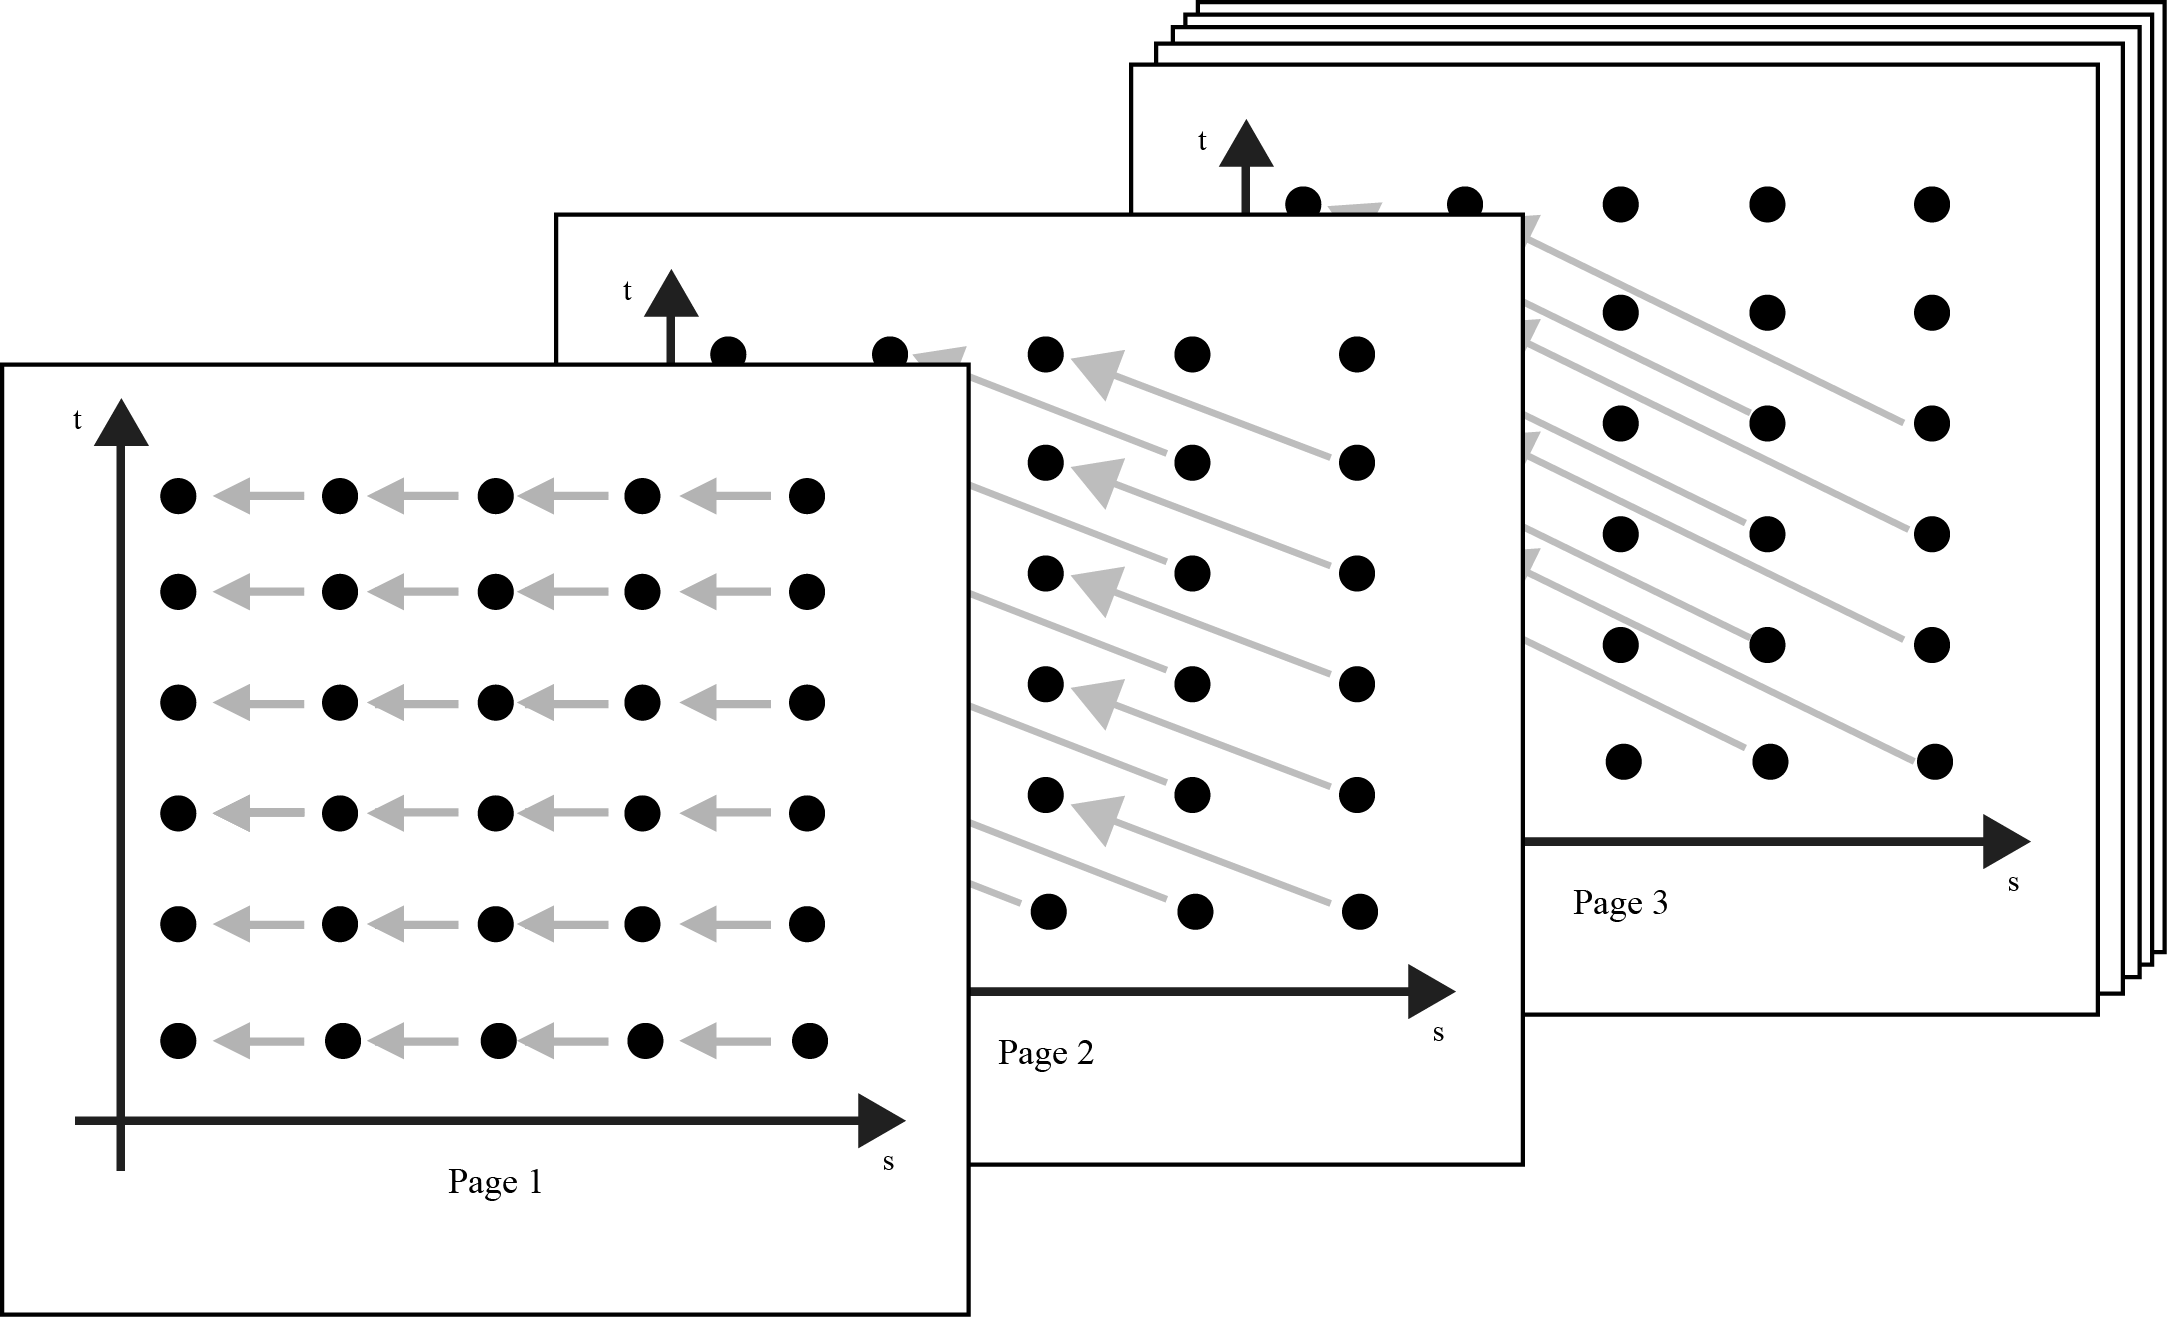
\includegraphics[width=\linewidth,height=0.45\textheight,keepaspectratio]{figures/cover.png}
  \end{center}
       \begin{minipage}{.35\linewidth}
    \begin{flushleft}
      \vspace{2em}
      {\fontsize{6pt}{2pt} \textit{Notes: These are notes live-tex'd
from a graduate course in Algebraic Number Theory taught by Paul Pollack
at the University of Georgia in Spring 2021. As such, any errors or
inaccuracies are almost certainly my own. } } \\
    \end{flushleft}
    \end{minipage}
    \hfill
    \begin{minipage}{.65\linewidth}
    \end{minipage}
  }







\begin{document}

\date{}
\author{D. Zack Garza}
\maketitle
\begin{flushleft}
\textit{D. Zack Garza} \\
\textit{University of Georgia} \\
  \textit{\href{mailto: dzackgarza@gmail.com}{dzackgarza@gmail.com}} \\
{\tiny \textit{Last updated:} 2021-03-02 }
\end{flushleft}


\newpage

% Note: addsec only in KomaScript
\addsec{Table of Contents}
\tableofcontents
\newpage

\def\contradiction
{
\tikz[baseline, x=0.2em, y=0.2em, line width=0.04em]
\draw (0,0) -- ({4*cos(45)},{4*sin(45)})
    (-1,1) -- ({-1 + 4*cos(45)},{1 + 4*sin(45)})
    (-1,3) -- ({-1 + 4*cos(315)},{3 + 4*sin(315)})
    (0,4) -- ({0 + 4*cos(315)},{4 + 4*sin(315)});
}

\def\contradiction
{
\tikz[baseline, x=0.2em, y=0.2em, line width=0.04em]
\draw (0,0) -- ({4*cos(45)},{4*sin(45)})
    (-1,1) -- ({-1 + 4*cos(45)},{1 + 4*sin(45)})
    (-1,3) -- ({-1 + 4*cos(315)},{3 + 4*sin(315)})
    (0,4) -- ({0 + 4*cos(315)},{4 + 4*sin(315)});
}

\hypertarget{thursday-january-14}{%
\section{Thursday, January 14}\label{thursday-january-14}}

See website for notes on books, intro to class.

\begin{itemize}
\item
  Youtube Playlist:
  \url{https://www.youtube.com/playlist?list=PLA0xtXqOUji8fjQysx4k8a6h-hOZ7x5ue}
\item
  Free copies of textbook:
  \url{https://www.dropbox.com/sh/rv5j222kn74bjhm/AABZ1qcR1rOnpaBsa5CL3P_Ea?dl=0\&lst=}
\item
  Course website: ?
\end{itemize}

Paul's description of the course:

``This course is an introduction to arithmetic''beyond
\({\mathbb{Z}}\)``, specifically arithmetic in the ring of''integers" in
a finite extension of \({\mathbb{Q}}\). (Among many other things) we'll
prove three important theorems about these rings:

\begin{itemize}
\tightlist
\item
  Unique factorization into ideals.
\item
  Finiteness of the group of ideal classes.
\item
  Dirichlet's theorem on the structure of the unit group."
\end{itemize}

\hypertarget{motivation}{%
\subsection{Motivation}\label{motivation}}

Solving Diophantine equations, i.e.~polynomial equations over
\({\mathbb{Z}}\).

\begin{example}[?]

Consider \(y^2 = x^3 + x\).

\begin{claim}

\((x, y) = (0, 0)\) is the only solution.

\end{claim}

To see this, write \(y^2 = x(x^2+1)\), which are relatively prime,
i.e.~no \(D\in {\mathbb{Z}}\) divides both of them. Why? If
\(d \mathrel{\Big|}x\) and \(d \mathrel{\Big|}x+1\), then
\(d\mathrel{\Big|}(x^2+1) + (-x) = 1\). It's also the case that both
\(x^2+1\) and \(x^2\) are squares (up to a unit), so \(x^2, x^2 + 1\)
are consecutive squares in \({\mathbb{Z}}\). But the gaps between
squares are increasing: \(1, 2, 4, 9, \cdots\). The only possibilities
would be \(x=0, y=1\), but in this case you can conclude \(y=0\).

\end{example}

\begin{example}[Fermat]

Consider \(y^2 = x^3-2\).

\begin{claim}

\((3, \pm 5)\) are the only solutions.

\end{claim}

Rewrite
\begin{align*}
x^3 = y^2+2 &= (y+ \sqrt{-2})(y - \sqrt{-2}) \\ 
&\in
{\mathbb{Z}}[\sqrt{-2}] \coloneqq\left\{{a+b\sqrt{-2} {~\mathrel{\Big|}~}a,b,\in {\mathbb{Z}}}\right\} \leq {\mathbb{C}}
.\end{align*}
This is a subring of \({\mathbb{C}}\), and thus at least an integral
domain. We want to try the same argument: showing the two factors are
relatively prime. A little theory will help here:

\begin{definition}[Norm Map]

For \(\alpha\in {\mathbb{Z}}[\sqrt{-2}]\) define
\(N \alpha = \alpha\mkern 1.5mu\overline{\mkern-1.5mu\alpha\mkern-1.5mu}\mkern 1.5mu\).

\end{definition}

\begin{lemma}[?]

Let \(\alpha, \beta \in {\mathbb{Z}}[\sqrt{-2}]\). Then

\begin{enumerate}
\def\labelenumi{\arabic{enumi}.}
\item
  \(N(\alpha \beta) = N(\alpha) N(\beta)\)
\item
  \(N( \alpha) \in {\mathbb{Z}}_{\geq 0}\) and \(N(\alpha) = 0\) if and
  only if \(\alpha= 0\).
\item
  \(N(\alpha) = 1 \iff \alpha\in R^{\times}\)
\end{enumerate}

\end{lemma}

\begin{proof}[?]

\begin{enumerate}
\def\labelenumi{\arabic{enumi}.}
\item
  Missing, see video (10:13 AM).
\item
  \(N(\alpha) = a^2 + 2b^2 \geq 0\), so this equals zero if and only if
  \(\alpha= \beta= 0\)
\item
  Write
  \(1 = \alpha\mkern 1.5mu\overline{\mkern-1.5mu\alpha\mkern-1.5mu}\mkern 1.5mu\)
  if \(N(\alpha) = 1 \in R^{\times}\). Conversely if
  \(\alpha\in R^{\times}\) write \(\alpha \beta = 1\), then
  \begin{align*} 
  1 = N(1) = N(\alpha \beta) = N(\alpha ) N(\beta ) \in {\mathbb{Z}}_{\geq 0} 
  ,\end{align*}
  which forces both to be 1.
\end{enumerate}

\end{proof}

\begin{claim}

The two factors \(y \pm \sqrt 2\) are \emph{coprime} in
\({\mathbb{Z}}[\sqrt{-2}]\), i.e.~every common divisor is a unit.

\end{claim}

\begin{proof}[?]

Suppose \(\delta\mathrel{\Big|}y\pm \sqrt{-2}\), then
\(y + \sqrt{-2} = \delta \beta\) for some
\(\beta\in {\mathbb{Z}}[\sqrt{-2}]\). Take norms to obtain
\(y^2 + 2 = N \delta N \beta\), and in particular

\begin{itemize}
\tightlist
\item
  \(N \delta y^2 +2\)
\item
  \(\delta \mathrel{\Big|}(y+ \sqrt{-2} ) - (y - \sqrt{-2} ) = 2 \sqrt{-2}\)
  and thus \(N \delta \mathrel{\Big|}N(2 \sqrt{-2} ) = 8\).
\end{itemize}

In the original equation \(y^2 = x^3-2\), if \(y\) is even then \(x\) is
even, and \(x^3 - 2 \equiv 0-2 \pmod 4 \equiv 2\), and so
\(y^2 \equiv 2 \pmod 4\). But this can't happen, so \(y\) is odd, and
we're done: we have \(N \delta\mathrel{\Big|}8\) which is even or 1, but
\(N \delta\mathrel{\Big|}y^2 +2\) which is odd, so \(N \delta = 1\).

\end{proof}

We can identify the units in this ring:
\begin{align*}
{\mathbb{Z}}[\sqrt{-2} ]^{\times}= \left\{{ a + b \sqrt{-2} {~\mathrel{\Big|}~}a^2 + 2b^2 = 1}\right\}
\end{align*}
which forces \(a^2 \leq 1, b^2 \leq 1\) and thus this set is
\(\left\{{\pm 1}\right\}\).

So we have \(x^3 = ab\) which are relatively primes, so \(a,b\) should
also be cubes. We don't have to worry about units here, since \(\pm 1\)
are both cubes. So e.g.~we can write
\begin{align*}
y + \sqrt{-2} = (a + b \sqrt{-2} )^3 = (a^3-6ab^2) + (3a^2b -2b^3) \sqrt{-2}
.\end{align*}
Comparing coefficients of \(\sqrt{-2}\) yields
\begin{align*} 1 = b(3a^2b - 2b^2) \in {\mathbb{Z}}\implies b \mathrel{\Big|}1
,\end{align*}
and thus \(b\in {\mathbb{Z}}^{\times}\),
i.e.~\(b\in \left\{{\pm 1}\right\}\). By cases:

\begin{itemize}
\item
  If \(b=1\), then \(1 = 3a^2 -2 \implies a^2 = 1 \implies a = \pm 1\).
  So
  \begin{align*}
  y = \sqrt{-2} = (\pm 1 + \sqrt{-2} )^3 = \pm 5 + \sqrt{-2}
  ,\end{align*}
  which forces \(y=\pm 5\), the solution we already knew.
\item
  If \(b = -1\), then \(1 = -(3a^2 - 1)\) which forces
  \(1=3a^2 \in {\mathbb{Z}}\), so there are no solutions.
\end{itemize}

\end{example}

\begin{example}[?]

Consider \(y^2 = x^3 - 26\). Rewrite this as
\begin{align*}
x^3 = y^2 + 26 = (y + \sqrt{-26} )(y - \sqrt{-26} )
,\end{align*}
then the same lemma goes through with \(2\) replaced by \(26\)
everywhere where the RHS factors are still coprime. Setting
\(y + \sqrt{-26} = (a + b \sqrt{-26} )^3\) and comparing coefficients,
you'll find \(b=1, a = \pm 3\). This yields \(x=35, y=\pm 207\). But
there are more solutions: \((x, y) = (3, \pm 1)\)! The issue is that we
used unique factorization when showing that \(ab\) is a square implies
\(a\) or \(b\) is a square (say by checking prime factorizations and
seeing even exponents). In this ring, we can have \(ab\) a cube with
\emph{neither} \(a,b\) a cube, even up to a unit.

\end{example}

\begin{question}

When does a ring admit unique factorization? Do you even \emph{need} it?

\end{question}

This will lead to a discussion of things like the \textbf{class number},
which measure the failure of unique factorization. In general, the above
type of proof will work when the class number is 3!

\hypertarget{lecture-2-tuesday-january-19}{%
\section{Lecture 2 (Tuesday, January
19)}\label{lecture-2-tuesday-january-19}}

Today: Ch.2 of the book, ``Cast of Characters''. Note that all rings
will be commutative and unital in this course.

Last time: looked at factorization in
\({\mathbb{Z}}[\sqrt 2], {\mathbb{Z}}[\sqrt{26}]\). Where do rings like
this come from?

\begin{definition}[Number Field]

A \textbf{number field} is a subfield \(K \subseteq {\mathbb{C}}\) such
that \([K: {\mathbb{Q}}] < \infty\).

\end{definition}

\begin{remark}

Some authors don't require \(K \subseteq {\mathbb{C}}\), but any finite
extension of \({\mathbb{Q}}\) will embed into \({\mathbb{C}}\) so
there's no harm in this extra requirement.

\end{remark}

\begin{example}[?]

\({\mathbb{Q}}[\sqrt[3]{2}, {\mathbb{Q}}[\sqrt 2, \sqrt[5]{7}]\) or
\({\mathbb{Q}}(\theta)\) where \(\theta\) is a root of \(x^5 - x - 1\)
(which you can check is irreducible. Now that the round vs.~square
brackets here won't make a difference, since we're adjoining algebraic
numbers.

\end{example}

\begin{proposition}[?]

Let \(K_{/{\mathbb{Q}}}\) be a finite extension, say of degree
\(n\coloneqq[K: {\mathbb{Q}}]\). Then there are \(n\) distinct
embeddings \footnote{An injective ring morphism.} of \(K\) into
\({\mathbb{C}}\)

\end{proposition}

\begin{proof}[?]

We have \(K_{/{\mathbb{Q}}}\), which is necessarily separable since
\(\operatorname{ch}({\mathbb{Q}}) = 0\). By the primitive element
theorem, we can write \(K = {\mathbb{Q}}(\theta)\) where \(\theta\) is a
root of some degree \(n\) irreducible polynomial
\(f(x) \in {\mathbb{Q}}[x]\). Since \({\mathbb{C}}\) is algebraically
closed, \(f\) splits completely over \({\mathbb{C}}\) as
\(f = \prod_{i=1}^n (x- \theta_i\) which each \(\theta_i \in CC\)
distinct since \(f\) was irreducible and we're in characteristic zero.
Then for each \(i\) there is an embedding \(K = {\mathbb{Q}}[\theta]\)
given by
\begin{align*}
\iota_i: {\mathbb{Q}}[\theta] &\hookrightarrow{\mathbb{C}}\\
g(\theta) &\mapsto g(\theta_i)
.\end{align*}
There are some easy things to check:

\begin{itemize}
\tightlist
\item
  This is well-defined: elements in \(K\) are polynomials in \(\theta\)
  but they all differ by a multiple of the minimal polynomial of
  \(\theta\),
\item
  This is an inject homomorphism and thus an embedding, and
\item
  For distinct \(i\) you get distinct embeddings: just look at the image
  \(\iota_i(\theta)\), these are distinct numbers in \({\mathbb{C}}\).
\end{itemize}

\end{proof}

\begin{definition}[Real and Nonreal embeddings]

Let \(K_{/{\mathbb{Q}}}\) be a finite extension of degree
\(n = [K : {\mathbb{Q}}]\). We'll say an embedding
\(\sigma:K \to {\mathbb{C}}\) is \textbf{real} if
\(\sigma(K) \subseteq {\mathbb{R}}\) , otherwise we'll say the embedding
is \textbf{nonreal}.

\end{definition}

\begin{remark}

If \(\sigma\) is a nonreal, then
\(\mkern 1.5mu\overline{\mkern-1.5mu\sigma\mkern-1.5mu}\mkern 1.5mu\) is
a nonreal embedding, so this embeddings come in pairs. As a consequence,
the total number of embeddings is given by \(n = r_1 + 2r_2\), where
\(r_1\) is the number of real embeddings and \(r_2\) is the number of
nonreal embeddings.

\end{remark}

\begin{example}[?]

Let \(K = {\mathbb{Q}}(\sqrt[3]{2})\). Here \(n=3\) since this is the
root of a degree 3 irreducible polynomial. Using the proof we can find
the embeddings: factor
\begin{align*}
x^3 - 2 = (x - \sqrt[3]{2})(x - \omega \sqrt[3]{2}) (x - \omega^2 \sqrt[3]{2})
.\end{align*}
where \(\omega = e^{2\pi i / 3}\) is a complex cube root of unity. We
can form an embedding by sending
\(\sqrt[3]{2} \to \omega^j \sqrt[3]{2}\) for \(j=0,1,2\). The case
\(j=0\) sends \(K\) to a subset of \({\mathbb{R}}\) and yields a real
embedding, but the other two will be nonreal. So \(r_1 = 1, r_2 = 1\),
and we have \(3 = 1 + 2(1)\) and this is consistent.

\end{example}

\begin{remark}

We've only been talking about fields, since unique factorization is
trivial since there are no primes. There are thus ``too many'' units,
compared to the rings we were considering before, so we'll restrict to
subrings. The question is: where is the arithmetic? Given a number field
\(K\), we want a ring \({\mathbb{Z}}_K\) that fits this analogy:

\begin{center}
\begin{tikzcd}
{\mathbb{Q}}\ar[dd] & \leadsto & K\ar[dd] \\
\\
{\mathbb{Z}}& \leadsto & {\mathbb{Z}}_K = ?
\end{tikzcd}
\end{center}

\end{remark}

\begin{definition}[Algebraic Numbers]

Given \(\alpha\in {\mathbb{C}}\) we say \(\alpha\) is an
\textbf{algebraic number} if and only if \(\alpha\) is algebraic over
\({\mathbb{Q}}\), i.e.~the root of some polynomial in
\({\mathbb{Q}}[x]\).

\end{definition}

\begin{remark}

We know that if we define
\(\mkern 1.5mu\overline{\mkern-1.5mu{\mathbb{Q}}\mkern-1.5mu}\mkern 1.5mu\coloneqq\left\{{\alpha\in {\mathbb{C}}{~\mathrel{\Big|}~}\alpha \text{ is algebraic over } {\mathbb{Q}}}\right\}\),
we can alternatively describe this as
\(\mkern 1.5mu\overline{\mkern-1.5mu{\mathbb{Q}}\mkern-1.5mu}\mkern 1.5mu= \left\{{ \alpha\in {\mathbb{C}}{~\mathrel{\Big|}~}[{\mathbb{Q}}(\alpha) : {\mathbb{Q}}] < \infty }\right\}\).
This is convenient because it's easy to see that algebraic numbers are
closed under sums and products, just using the ways degrees behave in
towers.

\end{remark}

\begin{corollary}[?]

\(\mkern 1.5mu\overline{\mkern-1.5mu{\mathbb{Q}}\mkern-1.5mu}\mkern 1.5mu\hookrightarrow{\mathbb{C}}\)
is a subfield and every number field is a subfield of
\(\mkern 1.5mu\overline{\mkern-1.5mu{\mathbb{Q}}\mkern-1.5mu}\mkern 1.5mu\).

\end{corollary}

These are still fields, so lets define some interesting subrings.

\begin{definition}[$\bar \ZZ$ ]

Define
\(\mkern 1.5mu\overline{\mkern-1.5mu{\mathbb{Z}}\mkern-1.5mu}\mkern 1.5mu\coloneqq\left\{{ \alpha\in {\mathbb{C}}{~\mathrel{\Big|}~}\alpha\text{ is the root of a monic polynomial }f\in {\mathbb{Z}}[x]}\right\}\).

\end{definition}

\begin{theorem}[$\bar \ZZ$ is a ring]

\(\mkern 1.5mu\overline{\mkern-1.5mu{\mathbb{Z}}\mkern-1.5mu}\mkern 1.5mu\)
is a ring, and in fact a domain since it's a subring of
\({\mathbb{C}}\).

\end{theorem}

We'll use an intermediate criterion to prove this:

\begin{proposition}[Integrality Criterion]

Let \(\alpha\in {\mathbb{C}}\) and suppose there is a finitely generated
\({\mathbb{Z}}{\hbox{-}}\)submodule of \({\mathbb{C}}\) with
\(\alpha M \subseteq M \neq 0\). Then
\(\alpha\in \mkern 1.5mu\overline{\mkern-1.5mu{\mathbb{Z}}\mkern-1.5mu}\mkern 1.5mu\),
i.e.~\(\alpha\) is the root of a monic polynomial with integer
coefficients.

\end{proposition}

\begin{proof}[of integrality criterion]

Chasing definitions, take \(M\) and choose a finite list of generators
\(\beta_1, \beta_2, \cdots, \beta_m\) for \(M\). Then
\(\alpha M \subseteq M \implies \alpha \beta_i \in M\) for all \(M\),
and each \(\alpha \beta_i\) is a \({\mathbb{Z}}{\hbox{-}}\)linear
combination of the \(\beta_i\) . I.e. we have
\begin{align*}
\alpha 
\begin{bmatrix}
\beta_1 
\\
\vdots  
\\
\beta_n  
\end{bmatrix}
= 
\begin{bmatrix}
a_{11} & a_{12} & \cdots
\\
a_{21} &  a_{22} & 
\\
 \vdots &  &\ddots  
\end{bmatrix}
\begin{bmatrix}
\beta_1 
\\
\vdots  
\\
\beta_n  
\end{bmatrix}
\coloneqq A \vec{\beta}
,\end{align*}
where \(A \in \operatorname{Mat}(n\times m, {\mathbb{Z}})\). We can
rearrange this to say that
\begin{align*}
\qty{ \alpha \operatorname{id}- A} 
\begin{bmatrix}
\beta_1 
\\
\vdots  
\\
\beta_n  
\end{bmatrix}
=
\mathbf{0}
.\end{align*}
Not all of the \(\beta_i\) can be zero since \(M\neq 0\), and thus
\(\alpha \operatorname{id}- A\) is singular and thus has determinant
zero, so \(\det(x \operatorname{id}- A)\Big|_{x=a} = 0\). We have
\begin{align*}
x\operatorname{id}- A = 
\begin{bmatrix}
x - a_{1,} &  & &
\\
&  x - a_{2, 2} & & 
\\
&  & \ddots &
\\
& &  & x - a_{m, m}
\end{bmatrix}
,\end{align*}
where the off-diagonal components are constants in \({\mathbb{Z}}\)
coming from \(A\). Taking the determinant yields a monic polynomial: the
term of leading degree comes from multiplying the diagonal components,
and expanding over the remaining minors only yields terms of smaller
degree. So \(\det (x\operatorname{id}- A) \in {\mathbb{Z}}[x]\) is
monic.

\end{proof}

\begin{proof}[of theorem]

We want to show that
\(\mkern 1.5mu\overline{\mkern-1.5mu{\mathbb{Z}}\mkern-1.5mu}\mkern 1.5mu\)
is a ring, and it's enough to show that

\begin{itemize}
\tightlist
\item
  \(1\in \mkern 1.5mu\overline{\mkern-1.5mu{\mathbb{Z}}\mkern-1.5mu}\mkern 1.5mu\),
  which is true since \(x-1\) is monic.
\item
  It's closed under \(+, \cdot\).
\end{itemize}

Note that the first property generalizes to
\({\mathbb{Z}}\subseteq \mkern 1.5mu\overline{\mkern-1.5mu{\mathbb{Z}}\mkern-1.5mu}\mkern 1.5mu\),
since \(x-n\) is monic for any \(n\in {\mathbb{Z}}\). For the second,
let
\(\alpha, \beta \in \mkern 1.5mu\overline{\mkern-1.5mu{\mathbb{Z}}\mkern-1.5mu}\mkern 1.5mu\).
Define \(M \coloneqq{\mathbb{Z}}[\alpha, \beta]\), then it's clear that
\((\alpha + \beta)M \subseteq M\) and \((\alpha \beta)M \subseteq M\)
since \({\mathbb{Z}}[\alpha, \beta]\) are polynomials in
\(\alpha, \beta\) and multiplying by these expression still yields such
polynomials. It only remains to check the following:

\begin{claim}

\(M\) is finitely-generated.

\end{claim}

\begin{proof}[?]

Let \(\alpha\) be a root of \(f \in {\mathbb{Z}}[x]\) and \(\beta\) a
root of \(g\), both monic with \(\deg f = n, \deg g = m\). We want to
produce a finite generating set for
\(M\coloneqq{\mathbb{Z}}[\alpha, \beta]\), and the claim is that the
following works:
\(\left\{{ \alpha^i \beta^j}\right\} _{\substack{0\leq i < n \\ 0 \leq j < m} }\),
i.e.~every element of \(M\) is some \({\mathbb{Z}}{\hbox{-}}\)linear
combination of these.

Note that this is clearly true if we were to include \(n, m\) in the
indices by collecting terms of any polynomial in \(\alpha, \beta\), so
the restrictions are nontrivial. It's enough to show that for any
\(0 \leq I, J \in {\mathbb{Z}}\), the term \(\alpha^I \beta^J\) is a
\({\mathbb{Z}}{\hbox{-}}\)linear combination of the restricted elements
above. Divide by \(f\) and \(g\) to obtain \(x^I = f(x) q(x) + r(x)\)
and \(x^J = g(x) \tilde q(x) \tilde r(x)\) where \(r(x) = 0\) or
\(\deg r < n\) and similarly for \(\tilde r\), where (importantly) all
of these polynomials are in \({\mathbb{Z}}[x]\).

We're not over a field: \({\mathbb{Z}}[x]\) doesn't necessarily have a
division algorithm, so why is this okay? The division algorithm only
requires inverting the leading coefficient, so in general \(R[x]\)
admits the usual division algorithm whenever the leading coefficient is
in \(R^{\times}\).

Now plug \(\alpha\) into the first equation to obtain
\(\alpha^I = r(\alpha)\) where \(\deg r < n\), which rewrite
\(\alpha^I\) as a sum of lower-degree terms. Similarly writing
\(\beta^J = r(\beta)\), we can express
\begin{align*}
\alpha^I \beta^J = r(\alpha) r(\beta)
,\end{align*}
which is what we wanted.

\end{proof}

\end{proof}

\begin{remark}

We've just filled in another part of the previous picture:

\begin{center}
\begin{tikzcd}
{\mathbb{Q}}\ar[dd] & K\ar[dd] & \mkern 1.5mu\overline{\mkern-1.5mu{\mathbb{Q}}\mkern-1.5mu}\mkern 1.5mu\ar[dd]\\
\\
{\mathbb{Z}}& {\mathbb{Z}}_K & \mkern 1.5mu\overline{\mkern-1.5mu{\mathbb{Z}}\mkern-1.5mu}\mkern 1.5mu
\end{tikzcd}
\end{center}

\end{remark}

\begin{definition}[Ring of Integers]

Define
\({\mathbb{Z}}_K = \mkern 1.5mu\overline{\mkern-1.5mu{\mathbb{Z}}\mkern-1.5mu}\mkern 1.5mu\cap K\),
the \textbf{ring of integers} of \(K\). Note that this makes sense since
the intersection of rings is again a ring.

\end{definition}

\begin{remark}

Why not just work in
\(\mkern 1.5mu\overline{\mkern-1.5mu{\mathbb{Z}}\mkern-1.5mu}\mkern 1.5mu\)?
It doesn't have the factorization properties we want, e.g.~there are no
irreducible elements. Consider \(\sqrt 2\), we can factor is into two
non-units (noting that \(\sqrt 2\) is not a unit) as
\(\sqrt{\sqrt 2} \cdot \sqrt{\sqrt 2}\), and it's easy to check that if
\(a\) is not a unit then \(\sqrt a\) is not a unit. So this would yield
arbitrarily long factorizations, and is thus not Noetherian.

\end{remark}

The following is a reality check, and certainly a property we would
want:

\begin{proposition}[The ring of integers of $\QQ$ is $\ZZ$ ]

\({\mathbb{Z}}_{\mathbb{Q}}= {\mathbb{Z}}\).

\end{proposition}

\begin{proof}[of proposition]

\(\subseteq\): easy, since
\({\mathbb{Z}}\subseteq \mkern 1.5mu\overline{\mkern-1.5mu{\mathbb{Z}}\mkern-1.5mu}\mkern 1.5mu\)
and \({\mathbb{Z}}\subseteq {\mathbb{Q}}\), and is thus in their
intersection \({\mathbb{Z}}_{\mathbb{Q}}\) .

\(\supseteq\) : Let
\(\alpha\in {\mathbb{Z}}_{\mathbb{Q}}= {\mathbb{Q}}\cap\mkern 1.5mu\overline{\mkern-1.5mu{\mathbb{Z}}\mkern-1.5mu}\mkern 1.5mu\)
, so \(\alpha\) is a root of
\(x^n - a_{n-1}x^{n-1} + \cdots + a_1x + a_0 \in {\mathbb{Z}}[x]\). We
know \(\alpha= a/b\) with \(a,b \in {\mathbb{Z}}\), and we can use the
rational root test which tells us that
\(a\mathrel{\Big|}a_0, b\mathrel{\Big|}1\), so
\(b = \pm 1, \alpha = a/\pm 1 = \pm a \in {\mathbb{Z}}\) and thus
\(\alpha \in {\mathbb{Z}}\).

\end{proof}

We'll want to study \({\mathbb{Z}}_K\) for various number fields \(K\),
but we'll need more groundwork.

\begin{proposition}[Easy criterion to check if an integer is algebraic]

Let
\(\alpha \in \mkern 1.5mu\overline{\mkern-1.5mu{\mathbb{Q}}\mkern-1.5mu}\mkern 1.5mu\),
then
\begin{align*} \alpha\in \mkern 1.5mu\overline{\mkern-1.5mu{\mathbb{Z}}\mkern-1.5mu}\mkern 1.5mu\iff \min_ \alpha \in {\mathbb{Z}}[x], \end{align*}
where \(\min_ \alpha(x)\) is the unique monic irreducible polynomial in
\({\mathbb{Q}}[x]\) which vanishes at \(\alpha\).

\end{proposition}

\begin{proof}[?]

\(\impliedby\): Trivial, if the minimal polynomial already has integer
coefficients, just note that it's already monic and thus
\(\alpha \in \mkern 1.5mu\overline{\mkern-1.5mu{\mathbb{Z}}\mkern-1.5mu}\mkern 1.5mu\)
by definition.

\(\implies\): Why should the minimal polynomial have \emph{integer}
coefficients? Choose a monic \(f(x) \in {\mathbb{Z}}[x]\) with
\(f(\alpha) = 0\), using the fact that
\(\alpha\in \mkern 1.5mu\overline{\mkern-1.5mu{\mathbb{Z}}\mkern-1.5mu}\mkern 1.5mu\)
, and factor \(f(x) = \prod_{i=1}^n (x- \alpha_i) \in {\mathbb{C}}[x]\).
Note that each
\(\alpha_i \in \mkern 1.5mu\overline{\mkern-1.5mu{\mathbb{Z}}\mkern-1.5mu}\mkern 1.5mu\)
since they are all roots of \(f\) (a monic polynomial in
\({\mathbb{Z}}[x]\)). Use the fact that \(\min_ \alpha(x)\) divides
every polynomial which vanishes on \(\alpha\) over \({\mathbb{Q}}\), and
thus divides \(f\) (noting that this still divides over
\({\mathbb{C}}\)). Moreover, every root of \(\min_ \alpha(x)\) is a root
of \(f\), and so every such root is some \(\alpha_i\).

Now factor \(\min_ \alpha(x)\) over \({\mathbb{C}}\) to obtain
\(\min_ \alpha(x) = \prod_{i=1}^m (x - \beta_i)\) with all of the
\(\beta_i \in \mkern 1.5mu\overline{\mkern-1.5mu{\mathbb{Z}}\mkern-1.5mu}\mkern 1.5mu\).
What coefficients appear after multiplying things out? Just sums and
products of the \(\beta_i\), so all of the coefficients are in
\(\mkern 1.5mu\overline{\mkern-1.5mu{\mathbb{Z}}\mkern-1.5mu}\mkern 1.5mu\)
. Thus
\(\min_ \alpha(x) \in \mkern 1.5mu\overline{\mkern-1.5mu{\mathbb{Z}}\mkern-1.5mu}\mkern 1.5mu[x]\).
But the coefficients are also in \({\mathbb{Q}}\) by definition, so the
coefficients are in
\(\mkern 1.5mu\overline{\mkern-1.5mu{\mathbb{Z}}\mkern-1.5mu}\mkern 1.5mu\cap{\mathbb{Q}}= {\mathbb{Z}}\)
and thus \(\min_ \alpha(x) \in {\mathbb{Z}}[x]\).

\end{proof}

\begin{example}[Showing an integer is not algebraic using minimal polynomials]

\(\sqrt{5}/ 3 \not\in \mkern 1.5mu\overline{\mkern-1.5mu{\mathbb{Z}}\mkern-1.5mu}\mkern 1.5mu\)
since \(\min_ \alpha(x) = x^2 - 5/9 \not\in {\mathbb{Z}}[x]\), so this
is not an algebraic integer.

\end{example}

\begin{proposition}[$\ff(\ZZ_K) = K$ ]

\envlist

\begin{enumerate}
\def\labelenumi{\alph{enumi}.}
\tightlist
\item
  \(\mkern 1.5mu\overline{\mkern-1.5mu{\mathbb{Z}}\mkern-1.5mu}\mkern 1.5mu\)
  has
  \(\mkern 1.5mu\overline{\mkern-1.5mu{\mathbb{Q}}\mkern-1.5mu}\mkern 1.5mu\)
  as its fraction field, and
\item
  For any number field \(K\), \({\mathbb{Z}}_K\) has \(K\) as its
  fraction field.
\end{enumerate}

Moreover, both of these statements follow from:

\begin{enumerate}
\def\labelenumi{\alph{enumi}.}
\setcounter{enumi}{2}
\tightlist
\item
  If
  \(\alpha\in \mkern 1.5mu\overline{\mkern-1.5mu{\mathbb{Q}}\mkern-1.5mu}\mkern 1.5mu\)
  then
  \(d \alpha\in \mkern 1.5mu\overline{\mkern-1.5mu{\mathbb{Z}}\mkern-1.5mu}\mkern 1.5mu\)
  for some \(d\in {\mathbb{Z}}^{\geq 0}\)
\end{enumerate}

\end{proposition}

\begin{remark}

Thus the subring is ``big'' in the sense that if you allow taking
quotients, you recover the entire field. That \(c\implies a,b\): suppose
you want to write
\(\alpha \in \mkern 1.5mu\overline{\mkern-1.5mu{\mathbb{Q}}\mkern-1.5mu}\mkern 1.5mu\)
as \(\alpha=p/q\) with
\(p,q \in \mkern 1.5mu\overline{\mkern-1.5mu{\mathbb{Z}}\mkern-1.5mu}\mkern 1.5mu\).
Use \(c\) to produce
\(d\alpha\in \mkern 1.5mu\overline{\mkern-1.5mu{\mathbb{Z}}\mkern-1.5mu}\mkern 1.5mu\),
then just take \(d\alpha /d\). The same argument works for \(b\).

\end{remark}

\begin{exercise}[?]

Prove the proposition!

\end{exercise}

\begin{proposition}[?]

Suppose
\(\alpha\in \mkern 1.5mu\overline{\mkern-1.5mu{\mathbb{C}}\mkern-1.5mu}\mkern 1.5mu\)
and \(\alpha\) is a root of a monic polynomial in
\(\mkern 1.5mu\overline{\mkern-1.5mu{\mathbb{Z}}\mkern-1.5mu}\mkern 1.5mu [x]\).
Then
\(\alpha\in \mkern 1.5mu\overline{\mkern-1.5mu{\mathbb{Z}}\mkern-1.5mu}\mkern 1.5mu\).

\end{proposition}

\begin{remark}

This says that if a number \(\alpha\) is the root of a monic polynomial
whose coefficients are \emph{algebraic} integers, then \(\alpha\) itself
is an algebraic integer coefficients. This corresponds to the fact that
integral over integral implies integral in commutative algebra.

\end{remark}

\begin{exercise}[Prove the proposition.]

Prove this! Can use the integrality criterion (slightly challenging),
can also use Galois theory.

\end{exercise}

\hypertarget{lecture-3-thursday-january-21}{%
\section{Lecture 3 (Thursday, January
21)}\label{lecture-3-thursday-january-21}}

Today: roughly corresponds to chapter 3 in the book. Goal: do all of the
big theorems in the setting of quadratic number fields, then redo
everything for general number fields.

\hypertarget{quadratic-number-fields}{%
\subsection{Quadratic Number Fields}\label{quadratic-number-fields}}

Simplest case: \({\mathbb{Q}}\), a degree 1 number field, so the next
simplest case is degree 2.

\begin{definition}[Quadratic Number Fields]

A field \(K\) is a \textbf{quadratic number field} if and only if \(K\)
is a number field and \([K: {\mathbb{Q}}] = 2\).

\end{definition}

\begin{remark}

Some notation: if \(d\in {\mathbb{R}}^{\times}\), then \(\sqrt d\) means
the \emph{positive} square root of \(d\) if \(d \geq 0\), and if \(d<0\)
this denotes \(i\sqrt{{\left\lvert {d} \right\rvert}}\).

\end{remark}

\begin{proposition}[?]

If \(K\) is a quadratic number field, then
\(K = {\mathbb{Q}}(\sqrt{d})\) for some squarefree \footnote{\emph{Squarefree}
  means not divisible by \(n^2\) for any \(n > 1\in {\mathbb{Z}}\), or
  equivalently not divisible by the square of any primes.}
\(d\in {\mathbb{Z}}\). Moreover, this \(d\) is uniquely determined by
\(K\), so all quadratic number fields are parameterized by the set of
squarefree integers.

\end{proposition}

\begin{proof}[?]

\textbf{Existence}: Since \([K: {\mathbb{Q}}] = 2\), we have
\(K\supsetneq {\mathbb{Q}}\) so pick
\(\alpha\in K\setminus{\mathbb{Q}}\) then \(K = {\mathbb{Q}}(\alpha)\).
Note that we could also furnish this \(\alpha\) from the primitive
element theorem, although this is overkill here. So \(\alpha\) is a root
of some degree 2 \(p\in {\mathbb{Q}}[x]\), and by scaling coefficients
we can replace this by \(p\in {\mathbb{Z}}[x]\). So write
\(p(x) = Ax^2 + Bx + C\), in which case we can always write
\(\alpha = {-B \pm \sqrt{B^2 - 4AC} \over 2A}\) where \(A\neq 0\) since
this would imply that \(\alpha\in{\mathbb{Q}}\). Writing
\(\Delta\coloneqq B^2 - 4AC\), we have
\(K = {\mathbb{Q}}(\alpha) = {\mathbb{Q}}(\sqrt{\Delta})\). This is
close to what we want -- it's \({\mathbb{Q}}\) adjoin some integer --
but we'd like it to be squarefree.

Now let \(f\in {\mathbb{Z}}^{\geq 0}\) be chosen such that
\(f^2 \mathrel{\Big|}\Delta\) and \(f\) is as large as possible,
i.e.~the largest square factor of \(\Delta\). Writing
\(\Delta = f^2 - d\) where \(d\) is whatever remains. Then \(d\) must be
squarefree, otherwise if \(d\) had a square factor bigger than 1, say
\(d = r^2 d'\), in which case \(f^2 r^2 > f^2\) would be a larger factor
of \(\Delta\). So \(d\) is squarefree, and \(\Delta = f \sqrt d\) and
thus \({\mathbb{Q}}(\Delta) = {\mathbb{Q}}(\sqrt{d})\).

\textbf{Uniqueness}: Well use some extra machinery.

\begin{definition}[Norm and Trace]

Let \(K\) be a number field with \(K_{/{\mathbb{Q}}}\) Galois. For each
\(\alpha\in K\) define
\begin{align*}
N(\alpha) &\coloneqq\prod_{\sigma\in \operatorname{Gal}(K_{/{\mathbb{Q}}})} \sigma(\alpha) && \text{the norm} \\
\operatorname{Tr}(\alpha) &\coloneqq\sum_{\sigma\in \operatorname{Gal}(K_{/{\mathbb{Q}}})} \sigma(\alpha) && \text{the trace}
.\end{align*}

\end{definition}

\begin{remark}

Why use these kind of sum at all? Applying any element in the Galois
group just permutes the elements. Note that
\(N( \alpha), \operatorname{Tr}( \alpha)\) are
\(G(K_{/{\mathbb{Q}}}){\hbox{-}}\)invariant, and thus rational numbers
in \({\mathbb{Q}}\). The norm is multiplicative, and the trace is
additive and in fact \({\mathbb{Q}}{\hbox{-}}\)linear:
\(\operatorname{Tr}(a \alpha + b \beta) = a \operatorname{Tr}( \alpha) + b \operatorname{Tr}( \beta)\)
for all \(\alpha, \beta\in K\) and all \(a,b \in {\mathbb{Q}}\).

\end{remark}

What do the norm and trace look like for a quadratic field? We can write
\(K = \left\{{a + b \sqrt d {~\mathrel{\Big|}~}a,b \in {\mathbb{Q}}}\right\}\)
and there is a unique (non-identity) element
\(g\in \operatorname{Gal}(K_{/{\mathbb{Q}}})\) with
\(\sigma(a + b \sqrt d = a - b \sqrt{d}\). We'll refer to this
automorphism as \textbf{conjugation}. We can compute
\begin{align*}
N(a + b \sqrt{d} ) &= a^2 - db^2 \\
\operatorname{Tr}(a + b \sqrt{d} ) &= 2a
.\end{align*}

Returning to the proof, suppose otherwise that
\(K = {\mathbb{Q}}(\sqrt{d_1} ) = {\mathbb{Q}}( \sqrt{d_2} )\) with
\(d_1\neq d_2\) squarefree integers. Note that they must have the same
sign, otherwise one of these extensions would not be a subfield of
\({\mathbb{R}}\). We know \(\sqrt{d_1} \in {\mathbb{Q}}( \sqrt{d_2} )\)
and thus \(\sqrt{d_1} = a + b \sqrt{d_2}\) for some
\(a, b\in {\mathbb{Q}}\). Taking the trace of both sides, the LHS is
zero and the RHS is \(2a\) and we get \(a=0\) and
\(\sqrt{d_1} = b \sqrt{d_2}\). Write \(b = u/v\) with
\(u,v\in {\mathbb{Q}}\). Squaring both sides yields
\(v^2 d_1 = u^2 d_2\). Let \(p\) be a prime dividing \(d_1\); then since
\(d_1\) is squarefree there is only one copy of \(p\) occurring in its
factorization. Moreover there are an even number of copies of \(p\)
coming from \(v^2\), thus forcing \(d_2\) to have an odd power of \(p\).
This forces \(p\mathrel{\Big|}d_2\), and since this holds for every
prime factor \(p\) of \(d_1\), we get \(d_1 \mathrel{\Big|}d_2\) since
\(d_1\) is squarefree. The same argument shows that
\(d_2 \mathrel{\Big|}d_1\), so they're the same up to sign: but the
signs must match and we get \(d_1 = d_2\).

\end{proof}

Note that this results holds for every squarefree number not equal to 1.

\begin{question}

If \(K = {\mathbb{Q}}( \sqrt{d} )\), what is the ring of integers
\({\mathbb{Z}}_K\)? Some more machinery will help here.

\end{question}

\begin{definition}[The Field Polynomial of an Element]

Assume \(K_{/{\mathbb{Q}}}\) is a Galois number field and for
\(\alpha\in K\) define
\begin{align*}
\varphi_{\alpha}(x) \coloneqq\prod_{ \sigma\in \operatorname{Gal}(K_{/{\mathbb{Q}}})} \qty{ x - \sigma(\alpha)}
.\end{align*}

\end{definition}

\begin{remark}

For the same reasons mentioned for the norm/trace, we get
\(\varphi_{\alpha} \in {\mathbb{Q}}[x]\), and moreover
\(\varphi_{ \alpha } (\alpha) = 0\).

\end{remark}

When is \(\alpha\in {\mathbb{Z}}_K\)? We have the following criterion:

\begin{proposition}[?]

\begin{align*}
\alpha\in {\mathbb{Z}}_K \iff \varphi_{ \alpha } (x) \in {\mathbb{Z}}[x]
.\end{align*}

\end{proposition}

\begin{proof}[?]

\(\impliedby\): This is easy, since if \(\varphi_\alpha\) is a monic
polynomial with integer coefficients, meaning that \(\alpha\) is an
algebraic integer and thus in \({\mathbb{Z}}_K\).

\(\implies\): If \(\alpha \in {\mathbb{Z}}_K\) then it's the root of
some monic polynomial in \({\mathbb{Z}}[x]\), and the same is true for
\(\sigma(\alpha)\) and thus each
\(\sigma(\alpha) \in \mkern 1.5mu\overline{\mkern-1.5mu{\mathbb{Z}}\mkern-1.5mu}\mkern 1.5mu\).
So
\(\varphi_{ \alpha}(x) \in \mkern 1.5mu\overline{\mkern-1.5mu{\mathbb{Z}}\mkern-1.5mu}\mkern 1.5mu[x]\).
We said \(\varphi_{ \alpha}\) has coefficients in \({\mathbb{Q}}\) too,
and thus in
\(\mkern 1.5mu\overline{\mkern-1.5mu{\mathbb{Z}}\mkern-1.5mu}\mkern 1.5mu\cap{\mathbb{Q}}= {\mathbb{Z}}\).
So the problem is reduced to finding out when \(\varphi_{\alpha}(x)\)
has integer coefficients.

If \(\deg(K_{/{\mathbb{Q}}}) = n\), then
\begin{align*}
\varphi_{ \alpha}( \alpha) = \prod x- \sigma(\alpha) = x^n - \operatorname{Tr}(\alpha)x^{n-1} + \cdots + (-1)^n N( \alpha)
.\end{align*}
If \(n=2\), these are the only terms, and so if \(K\) is a quadratic
number field then \(\alpha\in K\) is in \({\mathbb{Z}}_K\) if and only
if \(\operatorname{Tr}( \alpha), N(\alpha) \in {\mathbb{Z}}\).

\end{proof}

\begin{example}[?]

Let \(K = {\mathbb{Q}}( \sqrt{5} )\), then is it true that
\({\mathbb{Z}}_K = {\mathbb{Z}}[\sqrt{5} ]\)? Since
\(1, \sqrt{5} \in {\mathbb{Z}}_K\), we have \(\supseteq\) since
\(1, \sqrt{5}\) are algebraic. The answer is \textbf{no}: take
\(\alpha\coloneqq{1 + \sqrt{5} \over 2}\), then \(N( \alpha) -4/4 = -1\)
and \(\operatorname{Tr}( \alpha) = 1\). These are integers, so
\(\alpha\in {\mathbb{Z}}_K\), and in fact \(\alpha\) is a root of
\(x^2 - x - 1 \in {\mathbb{Z}}[x]\).

\end{example}

\begin{theorem}[?]

Let \(K = {\mathbb{Q}}( \sqrt{d} )\) be a quadratic number field. Then
if \(d = 2,3 \pmod 4\), then
\({\mathbb{Z}}_K = \left\{{ a + b \sqrt{d} {~\mathrel{\Big|}~}a, b\in {\mathbb{Z}}}\right\}\).
If \(d=1 \pmod 4\), then
\({\mathbb{Z}}_K = \left\{{ {1 + b \sqrt{d} \over 2} {~\mathrel{\Big|}~}a,b\in {\mathbb{Z}},\, a\equiv b \pmod 2}\right\}\).

\end{theorem}

\begin{remark}

For \(d=1\), if \(a, b\) are even then we just recover the \(d=2,3\)
case, so we're picking up extra elements from when \(a,b\) both odd.

\end{remark}

\begin{proof}[?]

Let \(\alpha\in K\) and write \(\alpha = A + B \sqrt{d}\) with
\(A, B\in {\mathbb{Q}}\).

\begin{exercise}[?]

Check that \(N( \alpha), \operatorname{Tr}( \alpha) \in {\mathbb{Z}}\)
for both cases.

\end{exercise}

Assuming now that
\(N( \alpha), \operatorname{Tr}( \alpha) \in {\mathbb{Z}}\), then
\(A^2 - dB^2 \in {\mathbb{Z}}\). Multiply this by 2 to get
\((2A)^2 - d(2B)^2 \in 4{\mathbb{Z}}\). Recalling that
\(\operatorname{Tr}( \alpha) = 2 A\), we have
\((2A)^2 \in {\mathbb{Z}}\) and thus \(d(2B)^2 \in {\mathbb{Z}}\) as
well. The claim now is that \(2B \in {\mathbb{Z}}\): we know
\(2B\in {\mathbb{Q}}\). If \(2B\not\in {\mathbb{Z}}\), then the
denominator has some prime factor. This prime factor appears twice in
\((2B)^2\), and \(d(2B)^2 \in {\mathbb{Z}}\) then means that two copies
of \(p\) appear in \(d\) in order to cancel -- however, we assumed \(d\)
was squarefree. We now know that \(A, B \in {1\over 2}{\mathbb{Z}}\), so
write \(A = (1/2)a'\) and \(B = (1/2)b'\). Writing
\(\alpha= (1/2)a' + (1/2)b' \sqrt{d}\), we find that
\(N( \alpha) = ((a')^2 - d(b')^2) / 4 \in {\mathbb{Z}}\). So the
numerator is a multiple of 4, which yields
\((a')^2 \equiv d(b')^2 \pmod 4\). We proceed by cases.

\textbf{Case 1:} \(d = 2,3 \pmod 4\). If \(b'\) is odd then
\((b')^2 = 1\pmod 4\), which holds for any odd number. But then
\((a')^2 = d(b')^2 = d \pmod 4\), which is a problem -- squares modulo 4
can only be \(0\) or \(1\). This is a contradiction, so \(b'\) must be
even. Then \((b')^2 \pmod 4 = 0\), which forces \(a' \equiv 0 \pmod 4\)
and \(a'\) must be even. But if \(a', b'\) are both even,
\((1/2)a', (1/2)b'\in {\mathbb{Z}}\) and we obtain
\(\alpha\in {\mathbb{Z}}+ \sqrt{d} {\mathbb{Z}}\) .

\textbf{Case 2:} If \(d\equiv 1 \pmod 4\), then
\((a')^2 \equiv (b')^2 \pmod 4\). We can conclude that \(a', b'\) are
either both odd or both even, otherwise we'd get \(0\equiv 1 \pmod 4\),
and thus we can write \(a' \equiv b' \pmod 2\). But this was exactly the
condition appearing in the theorem.

\end{proof}

\begin{remark}

Let \(K\) be a quadratic number field. Then we can reformulate the
previous results as:

\begin{align*}
{\mathbb{Z}}_K = 
\begin{cases}
{\mathbb{Z}}[ \sqrt{d} ] &  d \equiv 2,3 \pmod 4
\\
{\mathbb{Z}}\left[{1 + \sqrt{d} \over 2}\right] & d \equiv 1 \pmod 4.
\end{cases}
\end{align*}

We've also shown that \({\mathbb{Z}}_K\) is a free
\({\mathbb{Z}}{\hbox{-}}\)module of rank 2, with basis either
\(\left\{{ 1, \sqrt{d} }\right\}\) or
\(\left\{{ 1, {1 + \sqrt{d} \over 2 } }\right\}\).

\end{remark}

\begin{remark}

What is true for general number fields? Important theorem:
\({\mathbb{Z}}_K\) is always a free \({\mathbb{Z}}{\hbox{-}}\)module,
i.e.~there always exists an \emph{integral basis}. Surprisingly, the
it's not always true that \({\mathbb{Z}}_K = {\mathbb{Z}}[\ell]\) for
\(\ell\) a single element.

\end{remark}

\hypertarget{lecture-4-wednesday-january-27}{%
\section{Lecture 4 (Wednesday, January
27)}\label{lecture-4-wednesday-january-27}}

Today: the failure of unique factorization. Roughly corresponds to
chapter 4: ``Paradise Lost''!

Setup: \(K\) is a quadratic field, a degree 2 extension of
\({\mathbb{Q}}\), which can be written as \(K = {\mathbb{Q}}(\sqrt{d})\)
with \(d\) squarefree. Last time, we completely described
\({\mathbb{Z}}_K\) (the algebraic integers in \(K\)):
\begin{align*}
{\mathbb{Z}}_K = 
\begin{cases}
{\mathbb{Z}}[ \sqrt{d} ] &  d \equiv 2,3 \pmod 4
\\
{\mathbb{Z}}\left[{1 + \sqrt{d} \over 2}\right] & d \equiv 1 \pmod 4.
\end{cases}
\end{align*}
We saw that the second admitted a different description as
\(\left\{{ {a + b \sqrt{d} \over 2}}\right\}\) where \(a,b\) are either
both even or both odd. Note that we can do interesting arithmetic in
\({\mathbb{Z}}_K\), but it's not necessarily well-behaved:
\({\mathbb{Z}}_K\) is not always a UFD. Letting \(d=-5\), we have
\({\mathbb{Z}}_K = {\mathbb{Z}}[ \sqrt{-5} ]\) where \(6\) factors in
two ways: \(6 = (1 + \sqrt{5} )(1 - \sqrt{-5} ) = (2)(3) = 6\).

Note that this isn't quite enough to show failure of unique
factorization, e.g.~we can factor \(16 = (4)(4) = (2)(8)\). Here you
should check that all 4 factors are irreducible, and that the factors on
the right aren't unit multiples of the ones on the left. For example,
\(21 = (-7)(-3) = (7)(3)\), but the factors only differ by the unit
\(-1\in {\mathbb{Z}}^{\times}\). The key to checking all of those: the
\textbf{norm map}:
\begin{align*}
N(a + b \sqrt{-5} ) = (a + b \sqrt{-5} ) (a - \sqrt{-5} ) = a^2 + 5b^2
.\end{align*}
where the second factor was the \emph{conjugate}, i.e.~the image of the
element under the nontrivial element of the Galois group of
\(K_{/{\mathbb{Q}}}\). If \(a + b \sqrt{-5} \in {\mathbb{Z}}_K\), then
\(N(a + b \sqrt{-5} \in {\mathbb{Z}}_{\geq 0}\) and is equal to zero if
and only if \(a + b \sqrt{-5} = 0\). Moreover, this is a unit if and
only if its norm is 1, \footnote{\(\impliedby\): If the norm is 1, the
  conjugate is the inverse. For the reverse direction, the argument was
  more complicated, and reduced to showing norms of units are \(\pm 1\),
  and positivity forces it to be \(1\).} i.e.~\(a^2 + 5b^2 = 1\), which
forces \(b=0\) and \(a=\pm 1\). So
\(U({\mathbb{Z}}[ \sqrt{-5} ] ) = \left\{{\pm 1}\right\}\).

We'll show one of the factors is irreducible, \(1 + \sqrt{-5}\). Recall
that \(x\in R\) a domain is \emph{irreducible} if and only if whenever
\(x = ab\), one of \(a,b\) is a unit. It itself is not a unit, since
\(N(1 + \sqrt{-5 }) = 6 \neq 1\). So suppose
\(1 + \sqrt{-5} = \alpha \beta\). Then
\begin{align*}
6 = N(\alpha \beta ) = N( \alpha) N( \beta)
,\end{align*}
and so up to reordering, we have \(N \alpha = 2, N \beta= 3\). Writing
\(\alpha= a + b \sqrt{-5}\) and taking norms yields \(2 = a^2 + 5b^2\),
which has no solutions: considering the equation \(\pmod 5\) yields
\(2\equiv a^2\), but \(2\) is not a square in
\({\mathbb{Z}}/5{\mathbb{Z}}\). \(\contradiction\)

Note that the only other way of factoring \(6\) is \(6=(1)(6)\), and
taking norms shows that one factor is a unit. So if we assume
\(\alpha, \beta\) aren't units, both \(N \alpha, N \beta > 1\), which
leads to the previous situation. By similar arguments, all 4 factors are
irreducible.

To see that the LHS factors aren't unit multiples of the RHS factors, we
can use the fact that the units are \(\pm 1\), and multiplying the LHS
by \(\pm 1\) can't yield \(2\) or \(3\). So this is a genuine
counterexample to unique factorization.

\hypertarget{factorization-theory}{%
\subsection{Factorization Theory}\label{factorization-theory}}

What went wrong in the previous example? We'll use a big of terminology
from an area of algebra called \emph{factorization theory}. Many
concepts related to divisibility can be discussed in this language!

\begin{definition}[Monoid]

A \textbf{monoid} is a nonempty set with a commutative associative
binary operation \(\cdot\) with an identity \(1\). We say a monoid is
\textbf{cancellative} if and only if whenever
\(\alpha \beta= \beta \alpha\) or \(\beta \alpha = \gamma \alpha\) then
\(\beta = \gamma\).

\end{definition}

\begin{definition}[Terminology for Cancellative Monoids]

A bunch of definitions: let \(M\) be a cancellative monoid.

\begin{itemize}
\tightlist
\item
  \(\alpha\mathrel{\Big|}\beta\) if and only if \(\beta= \alpha \gamma\)
  for some \(\gamma\).
\item
  \(\epsilon\) is a \textbf{unit} if \(\epsilon\mathrel{\Big|}1\).
\item
  \(\alpha , \beta\) are \textbf{associates} if
  \(\alpha = \epsilon \beta\) for some unit \(\epsilon\)
\item
  \(\pi\in M\) is \textbf{irreducible} if and only if \(\pi\) is a unit
  and whenever \(\pi= \alpha \beta\) then either \(\alpha\) or \(\beta\)
  is a unit.
\item
  \(\pi \in M\) is \textbf{prime} whenever
  \(\pi\mathrel{\Big|}\alpha \beta\) then \(\pi\mathrel{\Big|}\alpha\)
  or \(\pi\mathrel{\Big|}\beta\).
\item
  \(\delta \in M\) is a greatest common divisor of \(\alpha, \beta\) if
  and only if \(\delta\) is a common divisor that is divisible by every
  other common divisor.
\item
  \(M\) is a \textbf{unique factorization monoid} if and only if every
  nonunit element in \(M\) factors uniquely as a product of irreducibles
  (uniqueness up to order and associates).
\end{itemize}

\end{definition}

\begin{remark}

Given \(R\) an integral domain, then \(R\setminus\left\{{0}\right\}\)
with multiplication is a cancellative monoid. Moreover,
\(R\setminus\left\{{0}\right\}\) is a unique factorization monoid if and
only if \(R\) is a UFD.

\end{remark}

\begin{question}

How do you show something is a UFD?

\end{question}

How does this proof go for \({\mathbb{Z}}\)?

\begin{itemize}
\tightlist
\item
  Use existence of a division algorithm
\item
  Prove Euclid's lemma: every irreducible is prime
\item
  Use factorization into irreducibles and proceed by induction (writing
  out two factorizations and cancelling things out in a combinatorial
  way)
\end{itemize}

So we'd like

\begin{enumerate}
\def\labelenumi{\arabic{enumi}.}
\tightlist
\item
  To know that irreducibles are prime, and
\item
  Everything to factor into irreducibles.
\end{enumerate}

\begin{definition}[Atomic]

For \(M\) a cancellative monoid, \(M\) is \textbf{atomic} if every
nonunit element of \(M\) is a product of irreducibles.

\end{definition}

\begin{proposition}[?]

Let \(M\) be a cancellative monoid, then \(M\) is a UFM if and only if
\(M\) is atomic and every irreducible is prime in \(M\).

\end{proposition}

\begin{proof}[?]

Omitted -- no new ideas when compared to proof of unique factorization
in \({\mathbb{Z}}\).

\end{proof}

Note that in \({\mathbb{Z}}\), working in \({\mathbb{Z}}_{\geq 0}\) is
useful because the only positive unit is \(1\), and so any elements
differing by a unit are in fact equal. Can we emulate this for
cancellative monoids? The answer is yes, by modding out by the
equivalence relation of being equivalent up to a unit.

\begin{definition}[Reduced Monoid]

Define \(M_{\operatorname{red}}\coloneqq M/\sim\) where
\(a\sim b \iff a-b\in M^{\times}\). The operation on \(M\) descends to
well-defined operation on \(M_{\operatorname{red}}\), and irreducibles
and primes are the same in \(M\) and \(M_{\operatorname{red}}\).

\end{definition}

\begin{example}[?]

This is supposed to look like \({\mathbb{Z}}_{\geq 0}\), where
\(-7\in M \mapsto 7 \in M_{\operatorname{red}}\).

\end{example}

\begin{proposition}[?]

\(M\) is a UFM if and only if \(M_{\operatorname{red}}\) is a UFM if and
only if every element of \(M_{\operatorname{red}}\) factors uniquely as
a product of irreducibles, up to order.

\end{proposition}

What did this buy us? We didn't have to worry about associates in the
above statement, and the only unit is 1.

\begin{question}

Why isn't \({\mathbb{Z}}[ \sqrt{-5} ]\) is UFD?

\end{question}

\begin{answer}

It doesn't have enough elements to make unique factorization work!

\end{answer}

\begin{example}[?]

In \({\mathbb{Z}}^+\), write \(210 = 21\cdot 10 = 14 \cdot 15\). These
two factorizations differ but admit a common refinement to
\((7\cdot 3)(2\cdot 5) = (7\cdot 2)(3\cdot 5)\), where it becomes clear
that these factorizations are equal up to ordering. This is
\textbf{Euler's Four Number Theorem}, which turns out to be equivalent
to unique factorization.

\end{example}

\begin{theorem}[?]

Let \(M\) be a cancellative atomic reduced monoid. Then \(M\) is a UFM
if and only if whenever \(\alpha, \beta, \gamma, \delta \in M\) such
that \(\alpha \beta = \gamma \delta\), there are
\(\rho, \sigma, \tau, \nu\) with
\begin{align*}
\alpha &= \rho \sigma \\
\beta &= \tau \nu \\
\gamma &= \rho \tau \\
\delta &= \sigma \nu
.\end{align*}

Note that plugging these in on the LHS and RHS respectively yield the
same factors, just reordered.

\end{theorem}

\begin{proof}[?]

Omitted, exercise in chasing definitions. The interesting part is that
you can go backward!

\end{proof}

Let
\(M_{\operatorname{red}} \coloneqq\qty{{\mathbb{Z}}[ \sqrt{5} ] \setminus\left\{{0}\right\}}_{\operatorname{red}}\),
motivated by the fact that \({\mathbb{Z}}[ \sqrt{-5} ]\) is not a UFD if
\({\mathbb{Z}}[ \sqrt{-5} ] \setminus\left\{{0}\right\}\) is not a UFM,
or equivalently its reduction is not a UFM. Then \(M\) is a not a UFM.
Noting that \(M\) is reduced under an equivalence relation, write
\(\left\langle{ \alpha}\right\rangle\) for the class of \(\alpha\) in
\(M\) for any \(\alpha\in {\mathbb{Z}}[ \sqrt{-5} ]\).

Our original counterexample for unique factorization now reads
\begin{align*}
\left\langle{ 1 + \sqrt{-5} }\right\rangle \left\langle{ 1 - \sqrt{5} }\right\rangle = \left\langle{2}\right\rangle \left\langle{3}\right\rangle
.\end{align*}
This is still a counterexample since these pairs admit no common
refinement.

Why are there ``not enough elements'' in \({\mathbb{Z}}[ \sqrt{-5} ]\)?
Recall that for integral domains (as rings), two elements differ by a
unit precisely when they generate the same ideal. So we can think of
elements of \(M_{\operatorname{red}}\) as nonzero principal ideals of
\(M\), which we'll write as
\(\operatorname{Prin}( {\mathbb{Z}}[ \sqrt{-5} ])\). To make this set of
ideals into a monoid, one define
\(\left\langle{ \alpha }\right\rangle \left\langle{ \beta }\right\rangle= \left\langle{ \alpha \beta }\right\rangle\),
where it's easy to check that this is well-defined. So the failure of
unique factorization is a failure of factorization in this set of
ideals. We can embed this in a larger collection of ideals by just
deleting the word ``principal'', which will restore unique
factorization.

\begin{definition}[Multiplication of Ideals]

Let \(R\) be a commutative ring (always with 1). If
\(I, J {~\trianglelefteq~}R\) are ideals, we define
\begin{align*}
IJ \coloneqq\left\langle{ \left\{{ \alpha_i \beta_i {~\mathrel{\Big|}~}\alpha_i \in I, \beta_i \in J }\right\}}\right\rangle = \left\{{ \sum \alpha_i \beta_i {~\mathrel{\Big|}~}\alpha_i \in I, \beta_i \in J}\right\}
.\end{align*}

If \(R\) is a domain, define the monoid \(\operatorname{Id}(R)\) the
collection of nonzero ideals of \(R\) with the above multiplication.

\end{definition}

\begin{remark}

Note that the naive definition
\(IJ \coloneqq\left\{{ij{~\mathrel{\Big|}~}i\in I, j\in J}\right\}\) is
not necessarily an ideal, since it may not be closed under addition.
Taking the smallest ideal containing all products fixes this.

\end{remark}

\begin{proposition}[?]

Let \(R\) be a commutative ring. Then

\begin{itemize}
\tightlist
\item
  \(\cdot\) for ideals is commutative
\item
  \(\cdot\) for ideals is associative
\item
  The identity is \(\left\langle{ 1 }\right\rangle= R\).
\item
  Multiplication distributes over addition of ideals,
  i.e.~\(I(J+K) = IJ + IK\).
\item
  \(IJ \subseteq I \cap J\).
\item
  If \(I = \left\langle{ \alpha_1, \cdots, \alpha_j }\right\rangle\) and
  \(J = \left\langle{ \beta_1, \cdots, \beta_k }\right\rangle\) then
  \(IJ = \left\langle{ \alpha_1 \beta_1, \cdots, \alpha_j \beta_k }\right\rangle\)
  is generated by all of the \(jk\) pairwise products.
\item
  If \(R\) is a domain and \(I, J\) are nonzero then \(IJ\) is nonzero.
\end{itemize}

As a consequence, \(\operatorname{Id}(R)\) is a monoid when \(R\) is a
domain.

\end{proposition}

So instead of working in
\(\operatorname{Prin}( {\mathbb{Z}}[\sqrt{-5} ])\), we'll work in
\(\operatorname{Id}({\mathbb{Z}}[\sqrt{-5} ])\).

\begin{claim}

We can refine our bad factorizations.

\end{claim}

Define

\begin{itemize}
\tightlist
\item
  \(I\coloneqq\left\langle{ 1 + \sqrt{-5} , 2 }\right\rangle\)
\item
  \(I'\coloneqq\left\langle{ 1 - \sqrt{-5} , 2 }\right\rangle\)
\item
  \(J\coloneqq\left\langle{ 1 + \sqrt{-5} , 3 }\right\rangle\)
\item
  \(J'\coloneqq\left\langle{ 1 - \sqrt{-5} , 3 }\right\rangle\)
\end{itemize}

Then

\begin{itemize}
\tightlist
\item
  \(IJ = \left\langle{ 1 + \sqrt{-5} }\right\rangle\)\\
\item
  \(I'J' = \left\langle{ 1 - \sqrt{-5} }\right\rangle\)\\
\item
  \(JJ' = \left\langle{ 3 }\right\rangle\)
\item
  \(II' = \left\langle{ 2 }\right\rangle\)
\end{itemize}

We can then write
\begin{align*}
\left\langle{ 1 + \sqrt{-5} }\right\rangle \left\langle{ 1 - \sqrt{-5} }\right\rangle = \left\langle{ 2 }\right\rangle \left\langle{ 3 }\right\rangle \implies (IJ)(I'J') = (II')(JJ')    
,\end{align*}
where the same terms are occurring in a different order.

For an example of how to work these out, let's compute \(IJ\). We get
\begin{align*}
IJ 
&= \left\langle{ (1 + \sqrt{-5} )^2, 3(1 + \sqrt{-5} ), 2(1 + \sqrt{-5} ), 6 }\right\rangle  \\
&= \left\langle{ 1 + \sqrt{-5} }\right\rangle \left\langle{ 1 + \sqrt{-5} , 3, 2, 1 - \sqrt{-5} }\right\rangle \\  
&= \left\langle{ 1 + \sqrt{-5} }\right\rangle \left\langle{ 1 }\right\rangle  \\
&= \left\langle{ 1 + \sqrt{-5} }\right\rangle
,\end{align*}
using the fact that \(3-2=1\) is in the ideal on the second line.

We'll see later that this process allows you to recover unique
factorization in \({\mathbb{Z}}_K\) for any number field \(K\).

\hypertarget{ch.-5-euclidean-quadratic-fields-thursday-january-28}{%
\section{Ch. 5: Euclidean Quadratic Fields (Thursday, January
28)}\label{ch.-5-euclidean-quadratic-fields-thursday-january-28}}

\begin{remark}

In a first algebra course, one process that if \(R\) is a Euclidean
domain, then the arithmetic of \(R\) is very interesting:

\begin{itemize}
\tightlist
\item
  \(R\) is a PID, and as a consequence
\item
  \(R\) is a UFD
\end{itemize}

\end{remark}

\begin{definition}[Euclidean Domain]

A domain \(R\) is \textbf{Euclidean} if and only if there is a function
\(\varphi R\setminus\left\{{0}\right\}\to {\mathbb{Z}}^{\geq 0}\) such
that for all \(a,b\in R\) with \(b\neq 0\) there are \(q, r\in R\) with
\(a = bq + r\) with \(r=0\) or \(\varphi(r) < \varphi(b)\). \(\varphi\)
is referred to as a \textbf{Euclidean function}.

\end{definition}

\begin{example}[Examples of Euclidean functions]

\envlist

\begin{itemize}
\tightlist
\item
  For \(R={\mathbb{Z}}\), one can take
  \(\varphi({\,\cdot\,}) \coloneqq{\left\lvert {{\,\cdot\,}} \right\rvert}\).
\item
  \(R = F[t]\) for \(F\) a field with
  \(\varphi({\,\cdot\,}) = \deg({\,\cdot\,})\).
\end{itemize}

\end{example}

\begin{remark}

Given a number field \(K\), does \({\mathbb{Z}}_K\) have nice
factorization, i.e.~is it a UFD? Not always, as we saw last time. If it
were Euclidean, then yes!

\end{remark}

\begin{question}

Which quadratic fields \(K\) have \(Z_K\) Euclidean?

\end{question}

\begin{definition}[Euclidean and Norm-Euclidean Number Fields]

If \(K\) is a quadratic field, then

\begin{itemize}
\item
  \(K\) is \textbf{Euclidean} if and only if \({\mathbb{Z}}_K\) is a
  Euclidean domain,
\item
  \(K\) is \textbf{norm-Euclidean} if and only if \({\mathbb{Z}}_K\) is
  Euclidean with respect to
  \(\varphi({\,\cdot\,}) \coloneqq{\left\lvert {N({\,\cdot\,})} \right\rvert}\).
\end{itemize}

\end{definition}

\begin{proposition}[Characterization of norm-Euclidean quadratic fields]

Let \(K\) be a quadratic field. Then \(K\) is norm-Euclidean if and only
if for all \(\beta\in K\) there is a \(\gamma\in {\mathbb{Z}}_K\) such
that \({\left\lvert { N(\beta- \gamma) } \right\rvert} < 1\). In other
words, \(K\) is norm-Euclidean if and only if every element can be
approximated by an element in \({\mathbb{Z}}_K\).

\end{proposition}

\begin{proof}[?]

\(\impliedby\): Let \(a,b \in {\mathbb{Z}}_k\) with \(b\neq 0\). Define
\(\beta\coloneqq a/b \in K\), then by assumption choose \(\gamma\) such
that \({\left\lvert {N({a\over b} - \gamma} \right\rvert}< 1\).
Multiplying both sides by \(N(b)\) and using the fact that
\(N({\,\cdot\,}), {\left\lvert {{\,\cdot\,}} \right\rvert}\) are
multiplicative, we have
\begin{align*}
{\left\lvert {N(a - b \gamma)} \right\rvert} < {\left\lvert {N(b)} \right\rvert} 
.\end{align*}
Then \(a = bq + r \coloneqq b \gamma + (a - b \gamma)\).

\end{proof}

\hypertarget{norm-euclidean-imaginary-quadratic-fields}{%
\subsection{Norm-Euclidean Imaginary Quadratic
Fields}\label{norm-euclidean-imaginary-quadratic-fields}}

\begin{remark}

Suppose \(K = {\mathbb{Q}}( \sqrt{d} )\) with \(d<0\) squarefree, so we
can write
\begin{align*}
K = \left\{{ a + b \sqrt{d} {~\mathrel{\Big|}~}a,b, \in {\mathbb{Q}}}\right\}
K = \left\{{ a + b i\sqrt{{\left\lvert {d} \right\rvert}} {~\mathrel{\Big|}~}a,b, \in {\mathbb{Q}}}\right\} \subseteq {\mathbb{C}}
.\end{align*}
Geometrically, this is a dense subset of \({\mathbb{C}}\), so it's not
easy to draw. But we can draw \({\mathbb{Z}}_K\) -- what does it look
like? We know that \(d=2,3 \pmod 4\) then
\({\mathbb{Z}}_K = \left\{{a + b \sqrt{d} {~\mathrel{\Big|}~}a,b,\in {\mathbb{Z}}}\right\}\):

\begin{figure}
\centering
\resizebox{\columnwidth}{!}{%
\begin{tikzpicture}
    \draw [thick, gray,-latex] (-5, 0) -- (7, 0);% Draw x axis
    \draw [thick, gray,-latex] (0, -5) -- (0, 5);% Draw y axis

    \clip (-5,-5) rectangle (10cm,10cm); % Clips the picture...
    %\pgftransformcm{1}{0.6}{0.7}{1}{\pgfpoint{0cm}{0cm}}
          % This is actually the transformation matrix entries that
          % gives the slanted unit vectors. 
    \draw[style=help lines,dashed] (-14,-14) grid[step=2cm] (6,5);
          % Draws a grid in the new coordinates.
          %\filldraw[fill=gray, fill opacity=0.3, draw=black] (0,0) rectangle (2,2);
              % Puts the shaded rectangle
    \foreach \x in {--3,-2,-1,0,1,2}{% Two indices running over each
      \foreach \y in {-2,-1, ..., 2}{% node on the grid we have drawn 
        \node[draw,circle,inner sep=2pt,fill] at (2*\x,2*\y) {};
            % Places a dot at those points
      }
    }
        \node[draw,red, circle,inner sep=2pt,fill] at (0, 0) {};

    \draw [decorate,decoration={brace,amplitude=10pt},xshift=-4pt,yshift=0pt] (6.5,2.0) -- (6.5,0.1) node [black,midway,xshift=25pt] {\footnotesize $\sqrt{{\left\lvert {d} \right\rvert}}$};
    \draw [decorate,decoration={brace,amplitude=10pt},xshift=-4pt,yshift=0pt] (6.5,-0.1) -- (6.5,-2) node [black,midway,xshift=25pt] {\footnotesize $\sqrt{{\left\lvert {d} \right\rvert}}$};

\end{tikzpicture}
}
\end{figure}

When \(d \equiv 1 \pmod 4\), we have
\({\mathbb{Z}}_k = \left\{{ {1\over 2}(a + b \sqrt{d} ) {~\mathrel{\Big|}~}a,b,\in {\mathbb{Z}},\, a\equiv b \pmod 2}\right\}\).
On the real axis, if \(b=0\) then \(a\) is an even integer and
\(\left\{{(1/2)a}\right\}\) is all integers. To get the remaining
elements, we don't just shift up and down: setting \(b=1\) yields
elements that look like \((1/2)a + \sqrt{d}\) where \(a\) is odd, so we
get the following:

\begin{figure}
\centering
\resizebox{\columnwidth}{!}{%
\begin{tikzpicture}
    \draw [thick, gray,-latex] (-5, 0) -- (7, 0);% Draw x axis
    \draw [thick, gray,-latex] (0, -5) -- (0, 5);% Draw y axis

    \clip (-5,-5) rectangle (10cm,10cm); % Clips the picture...
    %\pgftransformcm{1}{0.6}{0.7}{1}{\pgfpoint{0cm}{0cm}}
          % This is actually the transformation matrix entries that
          % gives the slanted unit vectors. 
    \draw[style=help lines,dashed] (-14,-14) grid[step=2cm] (6,5);
          % Draws a grid in the new coordinates.
          %\filldraw[fill=gray, fill opacity=0.3, draw=black] (0,0) rectangle (2,2);
              % Puts the shaded rectangle
    \foreach \x in {--3,-2,-1,0,1,2}{% Two indices running over each
      \foreach \y in {-2,-1, ..., 2}{% node on the grid we have drawn 
        \node[draw,circle,inner sep=2pt,fill] at (2*\x,2*\y) {};
            % Places a dot at those points
      }
    }
\foreach \x in {--2,-3,-1,0,1,2,-2}{% Two indices running over each
      \foreach \y in {-2,-1, ..., 2}{% node on the grid we have drawn 
        \node[draw, circle,inner sep=2pt,fill] at (2*\x+1,2*\y+1) {};
            % Places a dot at those points
      }
    }
        \node[draw,red, circle,inner sep=2pt,fill] at (0, 0) {};

    \draw [decorate,decoration={brace,amplitude=10pt},xshift=-4pt,yshift=0pt] (6.5,1.0) -- (6.5,0.1) node [black,midway,xshift=25pt] {\footnotesize ${1\over 2} \sqrt{{\left\lvert {d} \right\rvert}}$};
    \draw [decorate,decoration={brace,amplitude=10pt},xshift=-4pt,yshift=0pt] (6.5,-0.1) -- (6.5,-1) node [black,midway,xshift=25pt] {\footnotesize ${1\over 2} \sqrt{{\left\lvert {d} \right\rvert}}$};
\draw [decorate,decoration={brace,amplitude=10pt},xshift=-4pt,yshift=0pt] (6.5,1.95) -- (6.5,1.05) node [black,midway,xshift=25pt] {\footnotesize ${1\over 2} \sqrt{{\left\lvert {d} \right\rvert}}$};

\end{tikzpicture}
}
\end{figure}

Now we can think of the criterion for an imaginary quadratic field to be
norm-Euclidean: what does it mean to be within norm 1 of an element of
\({\mathbb{Z}}_K\)? If \(z\in K\), we can write
\(N(z) = z \mkern 1.5mu\overline{\mkern-1.5muz\mkern-1.5mu}\mkern 1.5mu = {\left\lvert {z} \right\rvert}^2\),
and thus reformulate our criterion: \(K\) is norm-Euclidean if and only
if for all \(\beta\in K\) there exists a \(\gamma\in {\mathbb{Z}}_K\)
such that \({\left\lvert {\beta- \gamma} \right\rvert}<1\). Note this
this is the familiar geometric distance in \({\mathbb{C}}\).

\end{remark}

\begin{example}[?]

\({\mathbb{Q}}(i)\) is norm-Euclidean: the ring of integers is
\({\mathbb{Z}}(i)\), which is the integer lattice in \({\mathbb{C}}\).
Note one can cover \({\mathbb{C}}\) by open circles of radius 1:

\begin{figure}
\centering
\resizebox{\columnwidth}{!}{%
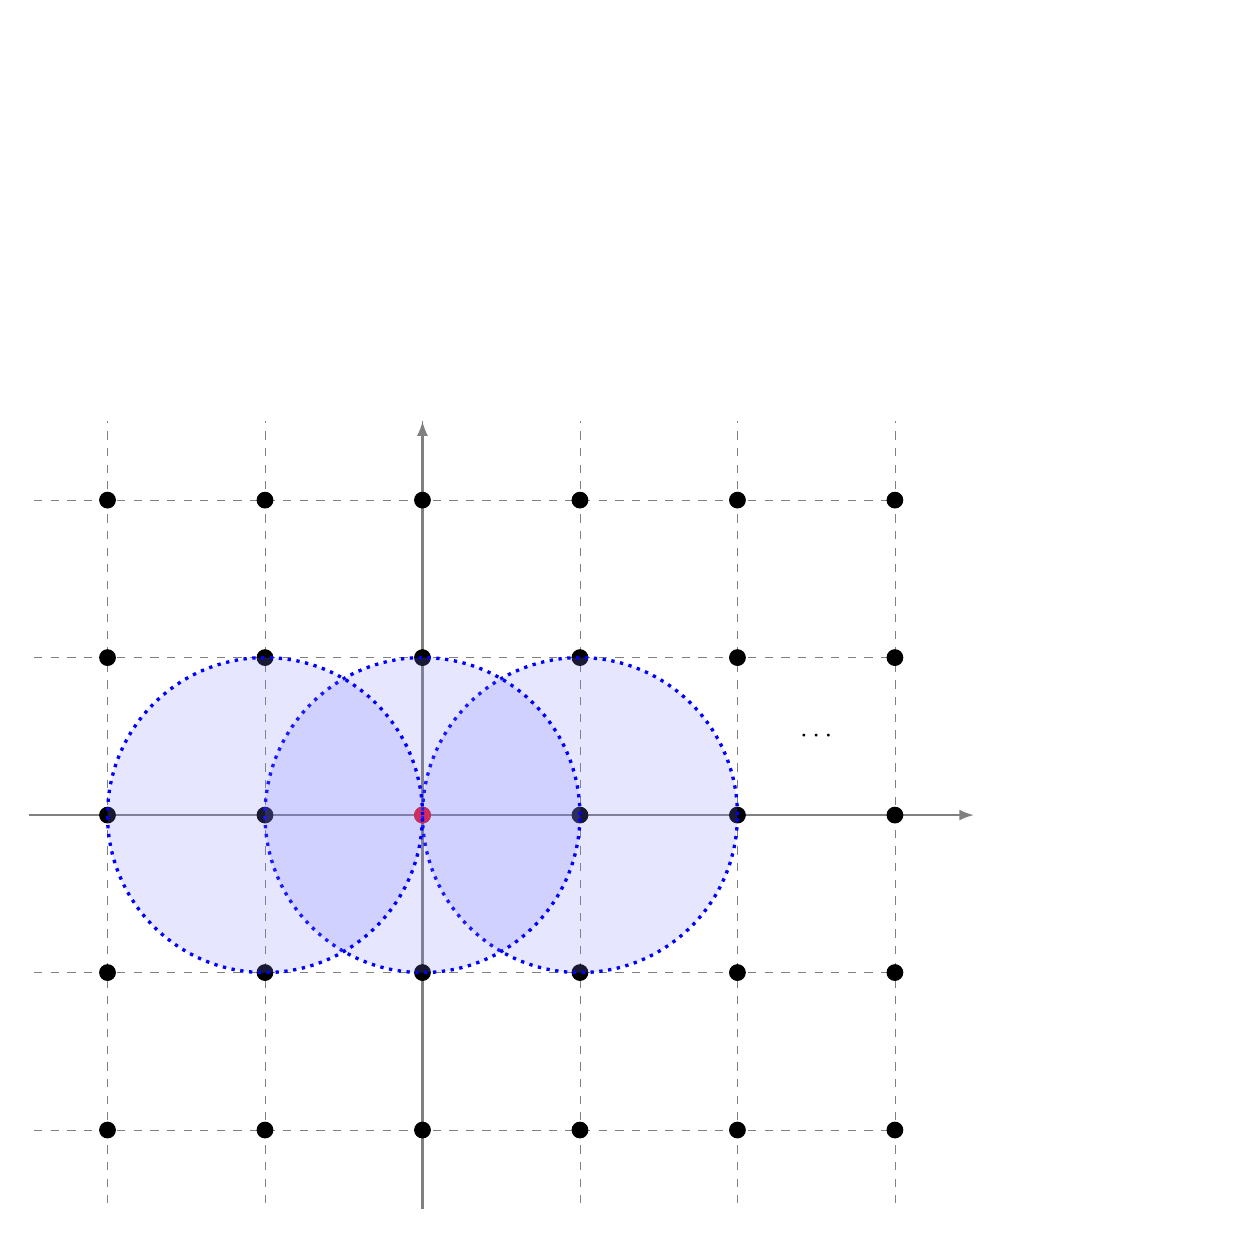
\begin{tikzpicture}
    \draw [thick, gray,-latex] (-5, 0) -- (7, 0);% Draw x axis
    \draw [thick, gray,-latex] (0, -5) -- (0, 5);% Draw y axis

    \clip (-5,-5) rectangle (10cm,10cm); % Clips the picture...
    %\pgftransformcm{1}{0.6}{0.7}{1}{\pgfpoint{0cm}{0cm}}
          % This is actually the transformation matrix entries that
          % gives the slanted unit vectors. 
    \draw[style=help lines,dashed] (-14,-14) grid[step=2cm] (6,5);
          % Draws a grid in the new coordinates.
          %\filldraw[fill=gray, fill opacity=0.3, draw=black] (0,0) rectangle (2,2);
              % Puts the shaded rectangle
    \foreach \x in {--3,-2,-1,0,1,2}{% Two indices running over each
      \foreach \y in {-2,-1, ..., 2}{% node on the grid we have drawn 
        \node[draw,circle,inner sep=2pt,fill] at (2*\x,2*\y) {};
            % Places a dot at those points
      }
    }
        \node[draw,red, circle,inner sep=2pt,fill] at (0, 0) {};

\filldraw[dotted, fill=blue!50, draw=blue, very thick, fill opacity=0.2] (2,0) circle (2cm);
\filldraw[dotted, fill=blue!50, draw=blue, very thick, fill opacity=0.2] (0,0) circle (2cm);
\filldraw[dotted, fill=blue!50, draw=blue, very thick, fill opacity=0.2] (-2,0) circle (2cm);
\node at (5, 1) {$\cdots$};
\end{tikzpicture}
}
\end{figure}

Continuing this way, every point with rational coordinates can be
covered by some open disc of radius 1:

\begin{figure}
\centering
\resizebox{\columnwidth}{!}{%
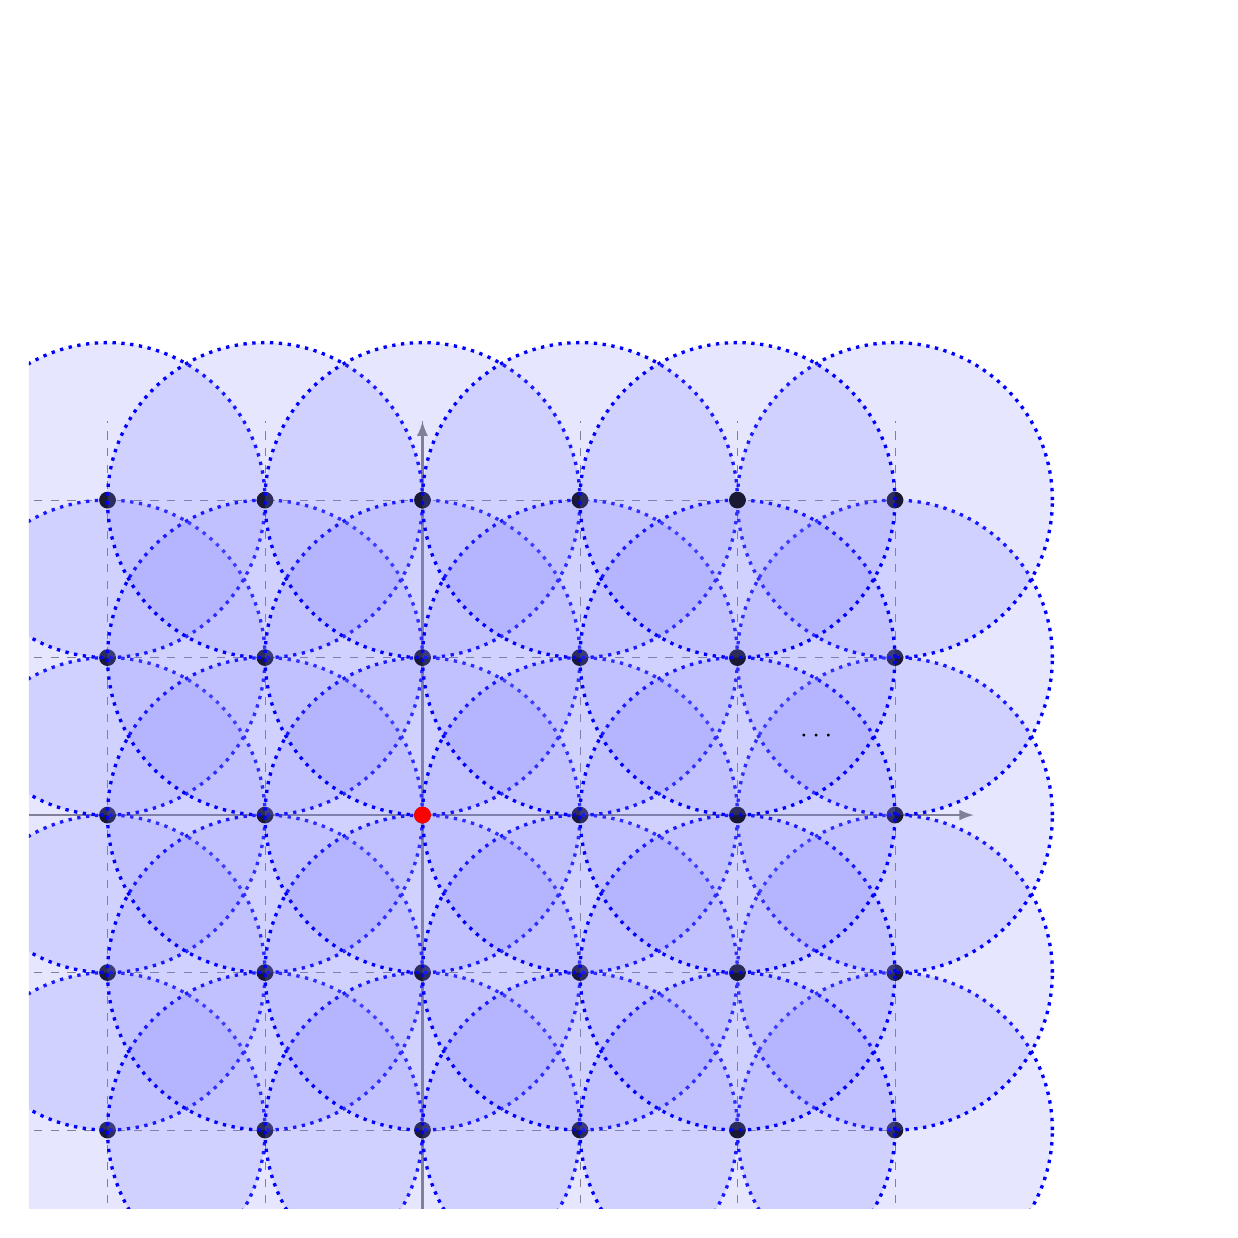
\begin{tikzpicture}
    \draw [thick, gray,-latex] (-5, 0) -- (7, 0);% Draw x axis
    \draw [thick, gray,-latex] (0, -5) -- (0, 5);% Draw y axis

    \clip (-5,-5) rectangle (10cm,10cm); % Clips the picture...
    %\pgftransformcm{1}{0.6}{0.7}{1}{\pgfpoint{0cm}{0cm}}
          % This is actually the transformation matrix entries that
          % gives the slanted unit vectors. 
    \draw[style=help lines,dashed] (-14,-14) grid[step=2cm] (6,5);
          % Draws a grid in the new coordinates.
          %\filldraw[fill=gray, fill opacity=0.3, draw=black] (0,0) rectangle (2,2);
              % Puts the shaded rectangle
    \foreach \x in {--3,-2,-1,0,1,2}{% Two indices running over each
      \foreach \y in {-2,-1, ..., 2}{% node on the grid we have drawn 
        \node[draw,circle,inner sep=2pt,fill] at (2*\x,2*\y) {};
\filldraw[dotted, fill=blue!50, draw=blue, very thick, fill opacity=0.2] (2*\x,2*\y) circle (2cm);

            % Places a dot at those points
      }
    }
        \node[draw,red, circle,inner sep=2pt,fill] at (0, 0) {};


\node at (5, 1) {$\cdots$};
\end{tikzpicture}
}
\end{figure}

\end{example}

\begin{remark}

Note that this doesn't work for arbitrary \(d\), since the distance
between the horizontal lines grows with \(d\). It's not hard to work out
the exact list where everything \emph{is} covered:

\end{remark}

\begin{theorem}[?]

\(K\) is norm-Euclidean if and only if
\(d\in \left\{{-1,-2,-3,-7,-11}\right\}\).

\end{theorem}

\begin{corollary}[?]

For these \(d\), \({\mathbb{Z}}_K\) is a PID and thus a UFD.

\end{corollary}

\begin{remark}

So we've classified all norm-Euclidean imaginary quadratic fields. What
about removing the word ``norm''? We restricted to
\({\left\lvert {N({\,\cdot\,})} \right\rvert}\) because there was a
particularly nice geometric interpretation, whereas being Euclidean
involves a mysterious \(\varphi\). Remarkably, it can be done, and it's
the same list!

\end{remark}

\begin{theorem}[Motzkin]

For \(K\) an imaginary quadratic field, \(K\) is Euclidean if and only
if \(d\in \left\{{-1,-2,-3,-7,-11}\right\}\).

\end{theorem}

\begin{remark}

If \({\mathbb{Z}}_K\) were never a PID in these cases, we could
immediately conclude it wasn't Euclidean either. But there are values of
\(d\) not on this list for which \({\mathbb{Z}}_K\) is a PID,
e.g.~\(d=-19\). Since \(-19 \equiv 1 \pmod 4\), one can write
\({\mathbb{Z}}_K = {\mathbb{Z}}\left[ {1 + \sqrt{-19} \over 2}\right]\),
and by Motzkin's theorem this is a PID which is not a Euclidean domain.

\end{remark}

We'll prove this theorem! First we need a few lemmas.

\begin{lemma}[?]

Let \(K\) be an imaginary quadratic field, then
\(U({\mathbb{Z}}_K) = \left\{{\pm 1 }\right\}\) except if \(d=-1, -3\).

\end{lemma}

\begin{proof}[of lemma (Important!)]

We know that the units \(u\) satisfy
\({\left\lvert {N(u)} \right\rvert} = 1\), and for imaginary quadratic
fields norms are non-negative, so we know \(N(u) = 1\). What are the
solutions this equation? Suppose \(d=2,3 \pmod 4\), then we can write
\(\alpha = a + b \sqrt{d}\) with \(a,b\in {\mathbb{Z}}\) and
\(1 = N \alpha = a^2 - db^2 = a^2 + {\left\lvert {d} \right\rvert}b^2\).
If \({\left\lvert {d} \right\rvert}= 1\) then this will have four
solutions: \((a, b) = (\pm 1, 0), (0, \pm 1)\). Otherwise if
\({\left\lvert {d} \right\rvert}> 1\) then \(b=0\) and
\(a^2=1 \implies a = \pm 1\) and thus \(\alpha = \pm 1\). So in this
case, the only units are \(\pm 1\), unless
\({\left\lvert {d} \right\rvert} = 1\). But the only negative squarefree
integer of absolute value 1 is \(-1\).

Suppose \(d \equiv 1 \pmod 4\). In this case, we need
\begin{align*}
1 = {a^2 + {\left\lvert {d} \right\rvert} b^2 \over 4} \implies a^2 + {\left\lvert {d} \right\rvert}b^2 = 4  
.\end{align*}
Note that \(d<0\) is \(1\pmod 4\), so it's possible that \(d=-3\) -- but
this was one of the exceptions in the theorem, so assume otherwise. Thus
\({\left\lvert {d} \right\rvert}\geq 7\), which forces
\(b=0 \implies a^2 = 4 \implies a = \pm 2\). Then \(\alpha= \pm 1\).

\end{proof}

\begin{remark}

For the excluded cases, the units can be explicitly computed. When
\(d=-1\), \(U({\mathbb{Z}}[i]) =\left\{{\pm 1, \pm i}\right\}\),
yielding 4 units. When \(d=-3\),
\begin{align*}
U\qty{{\mathbb{Z}}\left[ {1 + \sqrt{-3} \over 2 } \right]} = \left\{{\pm 1, {\pm 1 \pm \sqrt{-3} \over 2}}\right\}
,\end{align*}
yielding 6 units. Note that in the first case, these are exactly the 4th
roots of unity, and in the second case these are the sixth roots. This
is a general phenomenon that will appear again!

\end{remark}

\begin{lemma}[?]

Let \(K\) be any quadratic field and \(\alpha\in {\mathbb{Z}}_K\). Then
\(\# {\mathbb{Z}}_k / \left\langle{ \alpha }\right\rangle = {\left\lvert {N( \alpha )} \right\rvert}\).

\end{lemma}

\hypertarget{proof-of-motzkins-theorem}{%
\subsection{Proof of Motzkin's
Theorem}\label{proof-of-motzkins-theorem}}

\begin{proof}[of Motzkin's Theorem]

We want to show that being Euclidean implies \(d=-1,-2,-3,-7,-11\).
Suppose \({\mathbb{Z}}_K\) is Euclidean with respect to \(\varphi\).
Choose \(\beta\in {\mathbb{Z}}_K\) nonzero and not a unit with
\(\varphi(\beta)\) minimal among all such \(\beta\).

\begin{claim}

\begin{align*}
\# {\mathbb{Z}}_K / \left\langle{ \beta }\right\rangle \leq 3 
.\end{align*}

\end{claim}

\begin{proof}[of claim]

For any \(\alpha\in {\mathbb{Z}}_K\) and consider it in the quotient.
Since \({\mathbb{Z}}_K\) is Euclidean, we can write
\(\alpha = \beta + \gamma+ \rho\) where either \(\rho=0\) or
\(\varphi(\rho ) < \varphi (\beta )\). How can the second possibility
occur? \(\beta\) was chosen to have a minimal \(\varphi\) value, so the
only smaller elements are units. So \(\rho = 0\) or \(\rho\) is a unit.
Reducing \(\pmod\beta\), we obtain \(\alpha= \rho \pmod\beta\), and
hence
\(\# {\mathbb{Z}}_K / \left\langle{ \beta }\right\rangle \leq 1 + \# U({\mathbb{Z}}_K)\)
where the 1 comes from the zero element and everything else in the
quotient has a representative that is a unit. This is bounded above by
\(3\) when \(d\neq -1, -3\), which is one of the exclusions in the
theorem.

\end{proof}

Now we have \(N( \beta) \leq 3\) and this can be solved -- if \(d\) is
large, these solutions are widely distributed. If \(d = 2, 3 \pmod 4\)
then \(\beta= a + b \sqrt{d}\) with \(a, b \in ZZ\) and
\(a^2 + {\left\lvert {d} \right\rvert}b^2 \leq 3\). We can assume
\({\left\lvert {d} \right\rvert}> 3\), since \(d=-1, -2\) are excluded.
Then \(b=0\) is forced, and \(a = 0, \pm 1\). But why can't
\(\beta=0, \pm 1\)? It was chosen to be minimal among \emph{nonzero
nonunits}. \(\contradiction\)

If \(d \equiv 1 \pmod 4\), then \(\beta= {a + b \sqrt{d} \over 2}\)
where \(a,b\in {\mathbb{Z}},\, a\equiv b \pmod 2\). Then
\begin{align*}
{a^2 + {\left\lvert {d} \right\rvert}b^2 \over 4} \leq 3 \implies a^2 + {\left\lvert {d} \right\rvert}b^2 \leq 12  
.\end{align*}
Now considering that
\(-d\equiv 1 \pmod 4 \implies -d \in \left\{{ -3, -7, -11, \cdots}\right\}\),
the first three of which are on our list of exclusions. So we can assume
\({\left\lvert {d} \right\rvert}\geq 15\), which forces \(b=0\), \(a\)
must be even, and \(a^2 \leq 12\). So
\(a=0, \pm 2 \implies \beta= 0, \pm 1\). \(\contradiction\)

\end{proof}

\begin{remark}

What's the story for real quadratic fields? We understand norm-Euclidean
ones, although the proofs aren't nearly as simple. Things worked out
nicely here because we had circles in the plane; in the real case these
end up being complicated hyperbolas. One can prove that if \(d > 73\)
then \(K \coloneqq{\mathbb{Q}}(\sqrt d)\) is not norm-Euclidean. What
are the Euclidean real quadratic fields? The situation is much
different, and there are two open conjectures.

\end{remark}

\begin{conjecture}

For real quadratic fields \(K\), \({\mathbb{Z}}_K\) is a PID for
infinitely many \(d> 0\). We don't even know about to prove there are
just infinitely many \emph{number} fields satisfying this condition! We
believe this is true since it happens a positive proportion of the time
experimentally.

\end{conjecture}

\begin{conjecture}

If \({\mathbb{Z}}_K\) is a PID, then \({\mathbb{Z}}_K\) is Euclidean
with respect to some norm function. This is a consequence of a certain
generalization of the RH. This is not true for imaginary quadratic
fields. Why is it different here? The unit group plays a large role, and
is infinite here. The real conjecture is that for \(K\) any number
field, if \({\mathbb{Z}}_K\) is a PID with infinitely many units then
\({\mathbb{Z}}_K\) is Euclidean.

\end{conjecture}

\begin{remark}

There has been some progress, a result along the lines of there being at
most two exceptions, but we don't know if those exceptions exist.

\end{remark}

\hypertarget{ch.-6-ideal-theory-and-quadratic-fields-tuesday-february-02}{%
\section{Ch. 6: Ideal Theory and Quadratic Fields (Tuesday, February
02)}\label{ch.-6-ideal-theory-and-quadratic-fields-tuesday-february-02}}

Recall that if \(R\) is a domain, we defined \(\operatorname{Id}(R)\) as
the set of nonzero ideals of \(R\), which is a monoid. We want to get to
the following theorem:

\begin{theorem}[Fundamental Theorem of Ideal Theory (for Quadratic Fields)]

Let \(K\) be a quadratic field, then
\(\operatorname{Id}({\mathbb{Z}}_K)\) is a UFM.

\end{theorem}

\begin{remark}

This means that everything factors into irreducibles, and when you have
unique factorization, irreducible is the same as prime. Note that
``prime'' here means in this monoidal sense -- does this match up with
the existing notion of a prime ideal? I.e. that \(\mathfrak{p}\) is
prime if and only if \(R/ \mathfrak{p}\) is a domain, or
\(ab\in \mathfrak{p}\implies a,b \in \mathfrak{p}\)?

\end{remark}

\begin{proposition}[?]

``Prime'' in the usual ring-theoretic sense is equivalent to ``prime''
in the monoidal sense for \(\operatorname{Id}({\mathbb{Z}}_K)\).

\end{proposition}

\begin{remark}

Recall though that \(\operatorname{Id}({\mathbb{Z}}_K)\) is a reduced
monoid, so the only unit is the identity, so uniqueness is just up to
ordering and doesn't involve additional units. We can restart the unique
factorization theorem:

\end{remark}

\begin{proposition}[?]

Every nonzero ideal of \({\mathbb{Z}}_K\) factors uniquely as a product
of prime ideals in \({\mathbb{Z}}_K\).

\end{proposition}

Can we explicitly understand what ideals of \({\mathbb{Z}}_K\) look like
for quadratic fields?

\begin{definition}[Standard Bases of Ideals]

Let \(K = {\mathbb{Q}}(\sqrt{d})\), so
\({\mathbb{Z}}_K = {\mathbb{Z}}[\sqrt d]\) if \(d=2,3 \pmod 4\) or
\({\mathbb{Z}}\left[ {1 + \sqrt{d} \over 2} \right]\) if
\(d=1 \pmod 4\). Define \(\tau = \sqrt{d}\) or \((1 + \sqrt{d}) /2\)
accordingly and write \({\mathbb{Z}}_k = {\mathbb{Z}}[\tau]\).

\end{definition}

\begin{remark}

Note that \(\left\{{ 1, \tau }\right\}\) is a
\({\mathbb{Z}}{\hbox{-}}\)basis of \({\mathbb{Z}}_K\). An ideal of
\({\mathbb{Z}}_K\) is a submodule as a \({\mathbb{Z}}{\hbox{-}}\)module,
which is free, so any ideal is free of rank at most 2. Can we write down
such a basis?

\end{remark}

\begin{lemma}[?]

Let \(I\) be a nonzero ideal of \({\mathbb{Z}}_K\), then \(I\) contains
a nonzero integer and an element of the form \(a + b \tau\) where
\(b\neq 0\).

\end{lemma}

\begin{proof}[of lemma]

How to produce a nonzero rational integer: let \(\alpha\in I\) be
nonzero and take the norm. Then \(N \alpha\) is a nonzero integer, and
since
\(\mkern 1.5mu\overline{\mkern-1.5mu\alpha\mkern-1.5mu}\mkern 1.5mu\in {\mathbb{Z}}_K\)
we have
\(N \alpha = \alpha \mkern 1.5mu\overline{\mkern-1.5mu \alpha\mkern-1.5mu}\mkern 1.5mu \in I\).
Now since \(\tau\in {\mathbb{Z}}_K\) and \(I\) absorbs multiplication we
can set \(b \coloneqq N \alpha(\tau) \in I\).

\end{proof}

We wanted a nice description of bases for ideals -- here it is!

\begin{proposition}[Constructing a standard basis for an ideal]

Let \(I {~\trianglelefteq~}{\mathbb{Z}}_K\) be a nonzero ideal. Choose
\(n\in {\mathbb{Z}}^+\) such that
\(I \cap{\mathbb{Z}}= n{\mathbb{Z}}\).\footnote{Why does this \(n\)
  exist? Every ideal in \({\mathbb{Z}}\) is of the form
  \(n{\mathbb{Z}}\), and it's easy to check \(I \cap{\mathbb{Z}}\) is an
  ideal in \({\mathbb{Z}}\) since its an ideal of \({\mathbb{Z}}_K\)
  intersected with \({\mathbb{Z}}\). How do we know it's not the zero
  ideal? This is exactly given by the last lemma.} Choosing
\(B \in {\mathbb{Z}}^+\) such that
\(\left\{{ b\in {\mathbb{Z}}{~\mathrel{\Big|}~}a + b \tau\in I \text{ for some } a \in {\mathbb{Z}}}\right\} = B{\mathbb{Z}}\).\footnote{The
  LHS is the set of coefficients of \(\tau\), which is an ideal of
  \({\mathbb{Z}}\), and we can take it to be positive since the LHS is
  not the zero ideal by the lemma.} Since \(B\) is in the LHS, pick
\(A\in {\mathbb{Z}}\) with \(A + B\tau \in I\). Then
\(\left\{{n, A+B\tau}\right\}\) is a \({\mathbb{Z}}{\hbox{-}}\)basis for
\(I\). Any such basis is referred to as a \textbf{standard basis} for
\(I\)

\end{proposition}

\begin{remark}

Note that this is only determined up to \(A \pmod n\).

\end{remark}

\begin{proof}[?]

Take any element in \(I\), which can be represented as \(a + b \tau\),
we want to show that this can be expressed in terms of the proposed
basis. Note that \(B\mathrel{\Big|}b\) by its definition, since \(B\)
generated the ideal of \(\tau\) coefficients. So write \(b = Bs\), then
\begin{align*}
( a + b \tau) - (A + b \tau)s \in {\mathbb{Z}}\cap I = \left\langle{ n }\right\rangle 
.\end{align*}
So write this difference as \(nr\) for some \(r\in {\mathbb{Z}}\), then
rearranging yields
\begin{align*}
a + b \tau = nr + (A + B \tau)s
,\end{align*}
which is a \({\mathbb{Z}}{\hbox{-}}\)linear combination of the standard
basis elements. Uniqueness is easy and follows from the fact that every
element in \({\mathbb{Z}}_K\) has a unique representation in terms of
\(1, \tau\).

\end{proof}

\hypertarget{ideal-norms}{%
\subsection{Ideal Norms}\label{ideal-norms}}

In the previous section, we used the fact that for
\(a\in {\mathbb{Z}}_k\), the number of elements in
\({\mathbb{Z}}_K / \left\langle{ n }\right\rangle\) is
\({\left\lvert { N a } \right\rvert}\). That will be a consequence of
the theory we develop here.

\begin{definition}[?]

If \(I{~\trianglelefteq~}{\mathbb{Z}}_K\) is a nonzero ideal, define the
\textbf{norm of \(I\)} as
\(N(I) = {\left\lvert {{\mathbb{Z}}_K / I} \right\rvert}\).

\end{definition}

\begin{remark}

It's not completely obvious, but this quotient is always finite. We can
use the fact that \(I\leq {\mathbb{Z}}_K\) is a
\({\mathbb{Z}}{\hbox{-}}\)submodule of rank exactly 2. It's then a
general fact from algebra that \(A/B\) is finite when
\(\operatorname{rank}(A) = \operatorname{rank}(B)\), and there are ways
of figuring out the number of elements (see normal forms).

\end{remark}

\begin{proposition}[?]

Suppose that \(I{~\trianglelefteq~}{\mathbb{Z}}_K\) is a nonzero ideal
and let \(n, A+B \tau\) be a standard basis for \(I\). Then
\(N(I) = nB \in {\mathbb{Z}}^+\).

\end{proposition}

\begin{proof}[?]

Check that
\(\left\{{ a + b \tau {~\mathrel{\Big|}~}0\leq a \leq n,\, 0 \leq b \leq B}\right\}\)
is a complete and irredundant set of representatives for
\({\mathbb{Z}}_K/I\).

\end{proof}

\begin{remark}

So given a standard basis, it's easy to compute norms! What does this
have to do with the previous notion of norms for elements?

\end{remark}

\begin{theorem}[?]

Let \(I {~\trianglelefteq~}{\mathbb{Z}}_K\) be nonzero and define
\(\mkern 1.5mu\overline{\mkern-1.5muI\mkern-1.5mu}\mkern 1.5mu = \left\{{ \mkern 1.5mu\overline{\mkern-1.5mu\alpha \mkern-1.5mu}\mkern 1.5mu{~\mathrel{\Big|}~}\alpha \in I }\right\} {~\trianglelefteq~}{\mathbb{Z}}_K\).
Then
\(I \mkern 1.5mu\overline{\mkern-1.5muI\mkern-1.5mu}\mkern 1.5mu = \left\langle{ N(I) }\right\rangle\).

\end{theorem}

\begin{lemma}[?]

Let \(n, A + B \tau\) be a standard basis for \(I\). Then
\(B\mathrel{\Big|}n\) and \(B\mathrel{\Big|}A\).

\end{lemma}

\begin{proof}[of lemma]

Recall that \(B\) was a generator for \(\tau\) components of elements of
\(I\), so we just need to find an element of \(I\) with \(\tau\)
component \(n\), and \(n \tau \in I\) works.

Now compute \((A + B \tau) \tau\in I\). This is equal to
\begin{align*}
A \tau + B \tau^2
.\end{align*}
Note that this could in principle be done in cases: if
\(\tau = \sqrt{d}\), \(Bd\) would be an integer and \(A\) would be the
\(\tau\) coordinate. Then since \(B\) divides every \(\tau\)
coefficient, we'd be done. But let's try this in a more unified way: we
know \(\tau\) is a root of a monic degree 2 polynomial, namely
\((x - \tau) (x - \mkern 1.5mu\overline{\mkern-1.5mu\tau\mkern-1.5mu}\mkern 1.5mu) = x^2 - \operatorname{Tr}( \tau)x + N( \tau)\),
and thus we can write
\begin{align*}
\tau^2 = \operatorname{Tr}( \tau) \tau - N( \tau)
.\end{align*}
Substituting yields
\begin{align*}
(A + B \tau) \tau
&= A \tau + B \tau^2 \\
&= A \tau + B ( \operatorname{Tr}( \tau) \tau - N( \tau) ) \\
&= - B N( \tau) + (A + B \operatorname{Tr}( \tau ) ) \tau
.\end{align*}
The coefficient of \(\tau\) must be a multiple of \(B\), which forces
\(B\mathrel{\Big|}A\).

\end{proof}

\begin{proof}[of theorem]

Let \(n, A + B \tau\) be a standard basis for \(I\). Then
\(I = \left\langle{ n, A+ B \tau }\right\rangle\), which is a generating
set as a \({\mathbb{Z}}_K{\hbox{-}}\)module since they generate \(I\)
over \({\mathbb{Z}}\) and subset containment both ways can be readily
checked. We can then write
\(\mkern 1.5mu\overline{\mkern-1.5muI\mkern-1.5mu}\mkern 1.5mu = \left\langle{ n, A+B \mkern 1.5mu\overline{\mkern-1.5mu\tau \mkern-1.5mu}\mkern 1.5mu}\right\rangle\),
since conjugating ordinary integers doesn't change them. Using the
lemma, we can write
\begin{align*}
I &= \left\langle{ Bn', BA' + B \tau }\right\rangle\\
\mkern 1.5mu\overline{\mkern-1.5muI\mkern-1.5mu}\mkern 1.5mu &= \left\langle{ Bn', BA' + B \mkern 1.5mu\overline{\mkern-1.5mu\tau\mkern-1.5mu}\mkern 1.5mu }\right\rangle
.\end{align*}

We can factor out a \(B\) to get
\begin{align*}
I &= \left\langle{ B }\right\rangle \left\langle{ n', A' + \tau}\right\rangle \\  
\mkern 1.5mu\overline{\mkern-1.5muI\mkern-1.5mu}\mkern 1.5mu &= \left\langle{ B }\right\rangle \left\langle{ n', A' + \mkern 1.5mu\overline{\mkern-1.5mu\tau\mkern-1.5mu}\mkern 1.5mu }\right\rangle 
.\end{align*}

Now multiplying the two yields
\begin{align*}
I \mkern 1.5mu\overline{\mkern-1.5muI\mkern-1.5mu}\mkern 1.5mu = \left\langle{ B^2 }\right\rangle \left\langle{ (n')^2, n'(A' + \mkern 1.5mu\overline{\mkern-1.5mu \tau\mkern-1.5mu}\mkern 1.5mu ), n'(A' + \tau), N(A' + \tau) }\right\rangle  
.\end{align*}
It's tempting to factor out \(n'\), but it isn't obviously in the last
factor. But it is! Note that
\(N(A' + \tau) \in \left\langle{ A' + \tau, n' }\right\rangle\) and thus
\(B N(A' + gt) \in \left\langle{ B }\right\rangle \left\langle{ A' + \tau, n' }\right\rangle = I\).
But the first expression is an ordinary integer, i.e.~in
\(I \cap{\mathbb{Z}}= \left\langle{ n }\right\rangle\) and thus a
multiple of \(n\). So \(Bn' = n \mathrel{\Big|}BN(A' + \tau)\), and thus
\(n' \mathrel{\Big|}N(A' + \tau)\). So we can rewrite
\begin{align*}
I \mkern 1.5mu\overline{\mkern-1.5muI\mkern-1.5mu}\mkern 1.5mu 
&= \left\langle{ B^2 }\right\rangle \left\langle{ n' }\right\rangle \left\langle{ n', A' + \mkern 1.5mu\overline{\mkern-1.5mu \tau\mkern-1.5mu}\mkern 1.5mu , A' + \tau, { N(A' + \tau) \over n'} }\right\rangle   \\
&= \left\langle{ B^2 n' }\right\rangle 
\left\langle{ n', A' + \mkern 1.5mu\overline{\mkern-1.5mu \tau\mkern-1.5mu}\mkern 1.5mu , A' + \tau, { N(A' + \tau) \over  n'} }\right\rangle   
.\end{align*}

We can now note that \(B^2 n' = B^2(n/B) = nB = N(I)\). We've thus shown
that
\begin{align*}
I \mkern 1.5mu\overline{\mkern-1.5muI\mkern-1.5mu}\mkern 1.5mu 
= \left\langle{ N(I) }\right\rangle 
\left\langle{ n', A' + \mkern 1.5mu\overline{\mkern-1.5mu \tau\mkern-1.5mu}\mkern 1.5mu , A' + \tau, { N(A' + \tau) \over  n'} }\right\rangle   
.\end{align*}
We'd really like the second term to just be
\(\left\langle{ 1 }\right\rangle\). Note that this factor contains some
integers: \(n', N(A' + \tau)/n'\), and
\((A' + \mkern 1.5mu\overline{\mkern-1.5mu\tau\mkern-1.5mu}\mkern 1.5mu) + (A' + \tau) = \operatorname{Tr}(A' + \tau)\).
So let
\begin{align*}
J \coloneqq\left\langle{ n, N(A' + \tau)/n', \operatorname{Tr}(A' + \tau) }\right\rangle {~\trianglelefteq~}{\mathbb{Z}}
,\end{align*}
then it's enough to show
\(J = \left\langle{ 1 }\right\rangle {~\trianglelefteq~}{\mathbb{Z}}\).
Why? If so, \(1\) is a \({\mathbb{Z}}{\hbox{-}}\)linear combination of
these elements, but every \({\mathbb{Z}}{\hbox{-}}\)linear combination
is also a \({\mathbb{Z}}_K{\hbox{-}}\)linear combination. Every such
combination will be in the original ideal appearing in
\(I \mkern 1.5mu\overline{\mkern-1.5muI\mkern-1.5mu}\mkern 1.5mu\),
which we want to show is the unit ideal. We can write
\(J = d{\mathbb{Z}}\) where \(d\in {\mathbb{Z}}^+\) and suppose toward a
contradiction that \(d>1\). Consider
\(\alpha \coloneqq(A' + \tau) / d \in K\). Taking the trace is
\({\mathbb{Q}}{\hbox{-}}\)linear, so
\(\operatorname{Tr}( \alpha) = (1/d) \operatorname{Tr}(A' + \tau) \in {\mathbb{Z}}\).
This follows because the trace \(\operatorname{Tr}(A' + \tau)\) is in
\(J\), thus a multiple of \(d\). We can also compute
\(N \alpha = N(A' + \tau) / d^2\) using that
\(d\mkern 1.5mu\overline{\mkern-1.5mud\mkern-1.5mu}\mkern 1.5mu = d^2\)
since \(d\) is rational.

The claim is that \(N \alpha\) is also an integer: since
\(N(A' + \tau)/n', \operatorname{Tr}(A' + \tau)\) are in \(J\), \(d\)
divides both. So we know that
\(d^2 \mathrel{\Big|}(n') (N(A' + \tau) / n') = N(A' + \tau)\), which
forces \(N \alpha\in {\mathbb{Z}}\). So we know
\(N \alpha, \operatorname{Tr}\alpha \in {\mathbb{Z}}\), which forces
\(\alpha\in {\mathbb{Z}}_K\) since \(\alpha\) is a root of
\(x^2 - \operatorname{Tr}(\alpha) + N \alpha\). But \(\alpha\) can't be
in \({\mathbb{Z}}_K\), since these consist only of
\({\mathbb{Z}}{\hbox{-}}\)linear combinations of \(1, \tau\) -- however
here the coefficient of \(\tau\) is \(1/d \not \in {\mathbb{Z}}\), and
thus \(\alpha = A'/d + (1/d) \tau \not\in {\mathbb{Z}}_K\).

\end{proof}

\begin{remark}

This is a long proof! It's nice in that it's direct, but less nice in
that it required some clever steps. When we do the case for general
number fields, we'll be able to use a more conceptual approach that
avoids some of these computations. Many other facts fall out of these
theorem -- in fact, there are nice results as long as
\(I \mkern 1.5mu\overline{\mkern-1.5muI\mkern-1.5mu}\mkern 1.5mu\) is a
principal ideal.

\end{remark}

\hypertarget{chapter-6-fundamental-theory-of-ideal-theory-thursday-february-04}{%
\section{Chapter 6: Fundamental Theory of Ideal Theory (Thursday,
February
04)}\label{chapter-6-fundamental-theory-of-ideal-theory-thursday-february-04}}

\begin{remark}

Goal: establish unique factorization of ideals for quadratic fields. Let
\(K = {\mathbb{Q}}(\sqrt d)\) be a quadratic field and we let
\begin{align*}
\tau = 
\begin{cases}
\sqrt d & d \equiv 2,3 \pmod 4  
\\
{1 + \sqrt{d} \over 2} & d \equiv 1 \pmod 4.
\end{cases}
\end{align*}
In this case we saw that
\({\mathbb{Z}}_K = {\mathbb{Z}}+ {\mathbb{Z}}\tau = {\mathbb{Z}}[\tau]\).
We defined the norm of a nonzero ideal
\(I{~\trianglelefteq~}{\mathbb{Z}}_K\) by
\(N(I) = {\left\lvert {{\mathbb{Z}}_K/I} \right\rvert}\). The main
theorem was that
\(I \mkern 1.5mu\overline{\mkern-1.5muI\mkern-1.5mu}\mkern 1.5mu = \left\langle{ N(I)}\right\rangle\),
so the two definitions of norms are closely related. Some corollaries of
this theorem:

\end{remark}

\begin{corollary}[?]

Let \(I, J {~\trianglelefteq~}{\mathbb{Z}}_K\) be nonzero, then
\(N(IJ) = N(I) N(J)\).

\end{corollary}

\begin{proof}[of corollary]

Note that
\(IJ \mkern 1.5mu\overline{\mkern-1.5muIJ\mkern-1.5mu}\mkern 1.5mu = \left\langle{ N(IJ) }\right\rangle\)
on one hand, and on the other hand we can write this as
\(IJ \mkern 1.5mu\overline{\mkern-1.5muI\mkern-1.5mu}\mkern 1.5mu \mkern 1.5mu\overline{\mkern-1.5muJ\mkern-1.5mu}\mkern 1.5mu = I\mkern 1.5mu\overline{\mkern-1.5muI\mkern-1.5mu}\mkern 1.5mu J \mkern 1.5mu\overline{\mkern-1.5muJ\mkern-1.5mu}\mkern 1.5mu = \left\langle{ N(I) }\right\rangle \left\langle{ N(J) }\right\rangle = \left\langle{ N(I) N(J) }\right\rangle\).
So we know that
\(\left\langle{ N(IJ) }\right\rangle = \left\langle{ N(I) N(J) }\right\rangle\)
in \({\mathbb{Z}}_K\), how can we conclude that the generators are the
same? In a domain, they are the same up to a unit, so
\begin{align*}
{ N(IJ) \over N(I) N(J) } \in U({\mathbb{Z}}_K)
,\end{align*}
and thus this quotient is in
\({\mathbb{Z}}_K \cap{\mathbb{Q}}= {\mathbb{Z}}\). The same argument
shows that its reciprocal is also in \({\mathbb{Z}}\), so the ratio must
be a unit in \({\mathbb{Z}}\) and we have \(N(IJ) = \pm N(I) N(J)\). But
the norm counts something, so both sides must be positive.

\end{proof}

\begin{remark}

Note that if we knew \(I, J\) were comaximal, we could appeal to the
Chinese Remainder Theorem, but we don't need any assumptions on the
ideals for this proof.

\end{remark}

\begin{corollary}[?]

Let \(\alpha\in {\mathbb{Z}}_K \setminus\left\{{0}\right\}\), then
\begin{align*}
N( \left\langle{ \alpha }\right\rangle ) = {\left\lvert {N(\alpha)} \right\rvert}  = {\left\lvert {\alpha\mkern 1.5mu\overline{\mkern-1.5mu\alpha\mkern-1.5mu}\mkern 1.5mu} \right\rvert} 
.\end{align*}

\end{corollary}

\begin{proof}[of corollary]

We have
\begin{align*}
\left\langle{ N( \left\langle{ \alpha }\right\rangle  )}\right\rangle 
\left\langle{ \alpha }\right\rangle \left\langle{ \mkern 1.5mu\overline{\mkern-1.5mu\alpha \mkern-1.5mu}\mkern 1.5mu}\right\rangle 
&=
\left\langle{ \alpha }\right\rangle \left\langle{ \mkern 1.5mu\overline{\mkern-1.5mu\alpha \mkern-1.5mu}\mkern 1.5mu}\right\rangle \\
&=
\left\langle{ \alpha\mkern 1.5mu\overline{\mkern-1.5mu\alpha \mkern-1.5mu}\mkern 1.5mu}\right\rangle\\
&= \left\langle{ N \alpha }\right\rangle 
.\end{align*}
By the same argument as the previous corollary, this can only be true if
the generators are the same up to sign, so
\(N( \left\langle{ \alpha }\right\rangle = \pm N \alpha\).

\end{proof}

\hypertarget{unique-factorization-for-ideals}{%
\subsection{Unique Factorization for
Ideals}\label{unique-factorization-for-ideals}}

\begin{lemma}[Principal Multiple Lemma]

Let \(I {~\trianglelefteq~}{\mathbb{Z}}_K\setminus\left\{{0}\right\}\),
then there is another ideal
\(\tilde I {~\trianglelefteq~}{\mathbb{Z}}_K\setminus\left\{{0}\right\}\)
such that \(I \tilde I\) is principal.

\end{lemma}

\begin{proof}[of Principal Multiple Lemma]

Take
\(\tilde I \coloneqq\mkern 1.5mu\overline{\mkern-1.5muI\mkern-1.5mu}\mkern 1.5mu\),
since we proved that this is principal and generated by the norm.

\end{proof}

\begin{remark}

Why write this down when it's weaker than the previous theorem? In the
next proofs, we'll only really use that \(I\) times something is
principal.

\end{remark}

\begin{lemma}[Cancellation in the Monoid of Ideals]

Suppose that \(IJ = IJ'\) is an equation of nonzero ideals in
\({\mathbb{Z}}_K\) with \(I\) principal. Then \(J = J'\), so principal
ideals can be cancelled from both sides.

\end{lemma}

\begin{definition}[Dilation of Ideals]

If \(I {~\trianglelefteq~}{\mathbb{Z}}_K\), for any \(\alpha\in K\)
define
\begin{align*}
\alpha I \coloneqq\left\{{ \alpha \beta {~\mathrel{\Big|}~}\beta \in I }\right\} 
,\end{align*}
i.e.~scale or dilate the ideal \(I\) by the factor \(\alpha\). We'll
refer to this as the \textbf{dilation of \(I\) by \(\alpha\)}.

\end{definition}

\begin{remark}

Is this still an ideal in \({\mathbb{Z}}_K\)? It still contains zero, is
still closed under addition, and still absorbs multiplication by
elements in \(O_K\) -- however, it may not be a subset of
\({\mathbb{Z}}_K\), since we can dilate by any element in \(K\). For
example, for \(I \coloneqq 2{\mathbb{Z}}\) take \(\alpha\coloneqq 1/5\).
These are referred to as \textbf{fractional ideal}, i.e.~a
\({\mathbb{Z}}_K{\hbox{-}}\)submodule of \(K\). It is an ideal in
\({\mathbb{Z}}_K\) when it is contained in \({\mathbb{Z}}_K\).

\end{remark}

\begin{proof}[of cancellation in the monoid of ideals]

Write \(I = \left\langle{ \alpha }\right\rangle\). Then
\(\left\langle{ \alpha }\right\rangle J = \left\langle{ \alpha }\right\rangle J'\),
however the RHS is equal to the dilated ideal \(\alpha J'\) and the LHS
is \(\alpha J\). So dilate both sides by \(1/ \alpha\) to get
\(J = J'\).

\end{proof}

\begin{remark}

This was the easy case, when \(I\) was principal. What if \(I\) is not
principal?

\end{remark}

\begin{proposition}[$\Id(\ZZ_K)$ is Cancellative]

If \(IJ = IJ'\) then \(J = J'\), with no assumptions on \(I\).

\end{proposition}

\begin{proof}[?]

Choose \(\tilde I\) using the previous lemma and multiply it to both
sides to obtain
\begin{align*}
(I \tilde I) J = (I \tilde I) J'
.\end{align*}
Then since \(I\tilde I\) is principal, it can be cancelled using the
previous lemma.

\end{proof}

\hypertarget{proving-unique-factorization}{%
\subsubsection{Proving Unique
Factorization}\label{proving-unique-factorization}}

\begin{theorem}[To divide is to contain]

Let \(I, J\) be nonzero ideals of \({\mathbb{Z}}_K\), then
\begin{align*}
I \mathrel{\Big|}J \iff I \supseteq J
.\end{align*}

\end{theorem}

\begin{proof}[of theorem]

\(\implies\): This is true in any ring! If \(I\mathrel{\Big|}J\), then
\(J = IM\) where \(M {~\trianglelefteq~}{\mathbb{Z}}_K\), and by
definition \(IM \subseteq I\) and so \(J \subseteq I\).

\(\impliedby\): Suppose \(I \supseteq J\), we then want to find
\(B {~\trianglelefteq~}{\mathbb{Z}}_K\) with \(J = IB\). We'll proceed
by pretending we had such a \(B\) and seeing what it must be! If \(B\)
satisfies this equation, pick \(\tilde I\) where
\(I\tilde I = \left\langle{ \alpha}\right\rangle\), then
\begin{align*}
\tilde I J = \tilde I I B = \left\langle{ \alpha }\right\rangle B = \alpha B 
.\end{align*}
From here we can solve for \(B\) by dilating by \(1/ \alpha\), so
\(B = \alpha ^{-1} (\tilde I J)\). If we make this definition, does it
work?

First, do we have \(B \subseteq {\mathbb{Z}}_K\)? This amounts to check
that \(\tilde I H \subseteq \left\langle{ \alpha }\right\rangle\). This
is true, using the assumption \(J \subseteq I\), since
\(\tilde I J \subseteq \tilde I I = \left\langle{ \alpha }\right\rangle\).
So \(B\) is not a fractional ideal, and is an honest ideal of
\({\mathbb{Z}}_K\). We can also check that
\begin{align*}
IB 
&= I( \alpha ^{-1} \tilde I J) \\
& = \alpha^{-1}(I \tilde I J) \\
&= \alpha^{-1}( \left\langle{ \alpha }\right\rangle J ) \\
&= \alpha ^{-1} ( \alpha J) \\
&= J
,\end{align*}
using that dilation commutes with ideal multiplication.

\end{proof}

\begin{remark}

We now want to prove that \(\operatorname{Id}({\mathbb{Z}}_K)\) is a
UFM. If it's cancellative, we just need to check factorization into
irreducibles and that irreducibles are prime, i.e.~the analog of
Euclid's lemma.

\end{remark}

\begin{remark}

We'll use the fact that \(\operatorname{Id}({\mathbb{Z}}_K)\) is a
\emph{reduced} monoid, i.e.~the only unit is the identity
\(\left\langle{ 1 }\right\rangle\), the entire ring. This follows from
the fact that the product of ideals is contained in both factors, so
each factor would contain 1 and thus be the entire ring. We'll proceed
in two steps:

\end{remark}

\begin{proposition}[Unique Factorization]

\begin{enumerate}
\def\labelenumi{\arabic{enumi}.}
\item
  We'll show every element of \(\operatorname{Id}({\mathbb{Z}}_K)\)
  factors into irreducibles in \(\operatorname{Id}({\mathbb{Z}}_K)\),
  and
\item
  (Euclid's Lemma) Irreducibles in \(\operatorname{Id}({\mathbb{Z}}_K)\)
  are prime.
\end{enumerate}

\end{proposition}

\begin{remark}

We'll use the fact that it's reduced to avoid having to say ``non-unit
element'' in (1), since we have only one unit and we'll think of it as
the empty product. How do you prove (1)? The same way you prove it for
the integers: suppose you have a smallest counterexample. That can't be
prime, since a product of 1 prime is an allowable factorization, so this
factors into a product of two smaller things which necessarily can
\emph{not} be counterexamples by minimality. So the smaller factors
break up into primes -- but then so does their product, the original
counterexample, contradiction. The tricky part here is choosing what
``smaller'' should mean.

\end{remark}

\begin{proof}[of 1]

If not, choose \(I\) of smallest norm where \(I\) has no such
factorization. Then \(I \neq \left\langle{ 1 }\right\rangle\) since by
convention this does factor as the product of zero irreducibles, and
\(I\) is not irreducible since irreducibles count as their own
factorization. So we can factor \(I = AB\) with
\(A, B \neq \left\langle{ 1 }\right\rangle\). Taking norms yields
\begin{align*}
N(I) = N(AB) = N(A) N(B)
.\end{align*}
We'd like the norms of \(A, B\) to be smaller, since then we could apply
the inductive hypothesis. The only obstruction to this would be if
\(N(A) = 1\) and \(N(B) = N(I)\). But having norm 1 means that
\(A = \left\langle{ 1 }\right\rangle\), since this means the quotient
has one element, forcing it to be the zero ring. So everything in the
ring is zero mod the ideal, i.e.~in the ideal. So
\(1 < N(A), N(B) < N(I)\). Since \(I\) was the smallest counterexample,
both \(A\) and \(B\) can be factored into irreducibles, but then
concatenating the two factorizations yields a factorization for \(AB\).
\(\contradiction\)

\end{proof}

\begin{proof}[of 2: Euclid's Lemma]

Suppose \(P\) is irreducible in \(\operatorname{Id}({\mathbb{Z}}_K)\)
and suppose \(P \mathrel{\Big|}IJ\), we want to show \(P\) divides one
of these two. Suppose \(P\nmid I\), then \(P\) does not contain \(I\)
and \(P+I \supsetneq P\). This means that \(P+I\) is a \emph{proper
divisor} of \(P\), i.e.~it divides \(P\) but is not equal to \(P\). But
\(P\) was irreducible, so \(P+I\) is a unit, which forces
\(P + I = \left\langle{ 1 }\right\rangle\). Multiplying by \(J\) yields
\(PJ + IJ = J\). We said that \(P \mathrel{\Big|}IJ\) by assumption, so
\(IJ = PA\) for some nonzero ideal \(A\). So
\begin{align*}
J 
&= PJ + IJ \\
&= PJ + PA \\ 
&= P(J + A)
,\end{align*}
which shows that \(P\mathrel{\Big|}J\).

\end{proof}

\begin{remark}

Now running the exact same proof as for \({\mathbb{Z}}\) yields unique
factorization.

\end{remark}

\begin{exercise}[?]

Let \(P\) be a nonzero ideal of \(\operatorname{Id}({\mathbb{Z}}_K)\),
then \(P\) is monoidally prime in \(\operatorname{Id}({\mathbb{Z}}_K)\)
if and only if \(P\) is prime in the usual sense of prime ideals.

\emph{Hint: use ``to divide is to contain''.}

\end{exercise}

\hypertarget{chapter-7-preview}{%
\subsection{Chapter 7 Preview}\label{chapter-7-preview}}

\begin{remark}

This chapter is about understanding prime ideals in quadratic number
rings, i.e.~\({\mathbb{Z}}_K\) for quadratic fields. What are the
building blocks of the nonzero prime ideals?

\end{remark}

\begin{definition}[Prime ideal above a prime number]

Let \(P\) be a nonzero prime ideal, then \(P\) \textbf{lies above} the
rational prime \(p\) if and only if
\(P \supseteq \left\langle{ p }\right\rangle\). Equivalently,
\(p\in P\), or \(P\mathrel{\Big|}\left\langle{ p }\right\rangle\).

\end{definition}

\begin{theorem}[?]

Every nonzero prime ideal of \({\mathbb{Z}}_K\) lies above a unique
rational prime \(p\).

\end{theorem}

\begin{proof}[?]

Consider \(P \cap{\mathbb{Z}}{~\trianglelefteq~}{\mathbb{Z}}\). Tracing
through the definitions, if \(P\) is a prime ideal in
\({\mathbb{Z}}_K\), then this intersection is also prime in
\({\mathbb{Z}}\). Moreover \(P \cap Z \neq \left\{{ 0 }\right\}\), since
we can take any nonzero element \(\alpha \in P\), then
\(0\neq \alpha\mkern 1.5mu\overline{\mkern-1.5mu\alpha \mkern-1.5mu}\mkern 1.5mu\in {\mathbb{Z}}\)
and since \(P\) absorbs multiplication, this is still in \(P\). The
nonzero prime ideals of \({\mathbb{Z}}\) are of the form
\(n{\mathbb{Z}}\) with \(n\) prime, so
\(P \cap{\mathbb{Z}}= p{\mathbb{Z}}\) for some prime \(p\). But then
\(p\in P\) and \(P\) lies above \(p\). Why is this unique? If \(P\) lies
above \(q\), we would have \(q\in P \cap{\mathbb{Z}}= p {\mathbb{Z}}\)
and thus \(p\mathrel{\Big|}q\). But since these are both primes,
\(p=q\).

\end{proof}

\begin{remark}

If we want to figure out all of the prime ideals \(P\) of
\({\mathbb{Z}}_K\), we should see how \(\left\langle{ p }\right\rangle\)
factors, since each \(P\) shows up as a factor of some
\(\left\langle{ p }\right\rangle\). Thus the major question will be:
given \(p\), how does \(\left\langle{ p }\right\rangle\) factor into
prime ideals in \({\mathbb{Z}}_K\)?

\end{remark}

\hypertarget{ch.-7-prime-ideals-of-mathbbz_k-tuesday-february-09}{%
\section{\texorpdfstring{Ch. 7: Prime Ideals of \({\mathbb{Z}}_K\)
(Tuesday, February
09)}{Ch. 7: Prime Ideals of \{\textbackslash mathbb\{Z\}\}\_K (Tuesday, February 09)}}\label{ch.-7-prime-ideals-of-mathbbz_k-tuesday-february-09}}

Let \(K\) be a quadratic number field. Recall that if
\(P {~\trianglelefteq~}{\mathbb{Z}}_K\) is a prime then \(P\)
\textbf{lies above} \(p\in {\mathbb{Z}}\) if
\(P \supseteq \left\langle{ p }\right\rangle\). Equivalently,

\begin{itemize}
\tightlist
\item
  \(P\) contains \(p\), or
\item
  \(P \mathrel{\Big|}\left\langle{ p }\right\rangle\)
\end{itemize}

Last time we saw that every \(P\) lies above a unique \(p\). The
following diagram illustrates the situation:

\begin{center}
\begin{tikzcd}
    K && {{\mathbb{Z}}_K} && P \\
    \\
    {\mathbb{Q}}&& {\mathbb{Z}}&& p
    \arrow[no head, from=1-1, to=3-1]
    \arrow[no head, from=1-3, to=3-3]
    \arrow[no head, from=1-5, to=3-5]
\end{tikzcd}
\end{center}

\begin{quote}
\href{https://q.uiver.app/?q=WzAsNixbMCwwLCJLIl0sWzAsMiwiXFxRUSJdLFsyLDAsIlxcWlpfSyJdLFsyLDIsIlxcWloiXSxbNCwwLCJQIl0sWzQsMiwicCJdLFswLDEsIiIsMCx7InN0eWxlIjp7ImhlYWQiOnsibmFtZSI6Im5vbmUifX19XSxbMiwzLCIiLDAseyJzdHlsZSI6eyJoZWFkIjp7Im5hbWUiOiJub25lIn19fV0sWzQsNSwiIiwwLHsic3R5bGUiOnsiaGVhZCI6eyJuYW1lIjoibm9uZSJ9fX1dXQ==}{Link
to Diagram}
\end{quote}

If we want to determine all of the primes \(P\), we should consider
factoring all of the ideals \(\left\langle{ p }\right\rangle\) into
prime ideals of \({\mathbb{Z}}_K\). We have unique factorization for
prime ideals, so we can write
\(\left\langle{ p }\right\rangle = P_1 \cdots P_g\). Taking norms yields
\begin{align*}
N( \left\langle{ p }\right\rangle ) = \prod N(P_i) 
,\end{align*}
where we can identify the LHS as \(p^2\), since the norm for principal
ideals is the square of the generating element. Alternatively, we can
check the size of \({\mathbb{Z}}_K/ \left\langle{ p }\right\rangle\).
Note that \({\mathbb{Z}}_K\) is a free \({\mathbb{Z}}{\hbox{-}}\)module
on 2 generators, and we take both coordinates \(\pmod p\) to get
\(({\mathbb{Z}}/p{\mathbb{Z}})^2\). Since none of the terms on the RHS
are the unit ideal, none have norm 1, and so either

\begin{enumerate}
\def\labelenumi{\alph{enumi}.}
\item
  \(g=1\) and \(P_1 = \left\langle{ g }\right\rangle\) and
  \(\left\langle{ p }\right\rangle\) is prime. In this case we say \(p\)
  \textbf{is inert}.
\item
  If \(g=2\) and \(P_1 \neq P_2\), then we say \(p\)\$ \textbf{is
  split}.
\item
  If \(g=2\) and \(P_1 = P_2\)\textless{} then we say \(p\) \textbf{is
  ramified}.
\end{enumerate}

Let \(K = {\mathbb{Q}}( \sqrt{d} )\) and \(\tau\) as usual. We can
compute its minimal polynomial:
\begin{align*}
\min_\tau(x) = 
\begin{cases}
x^2 - d & d \equiv 2,3 \pmod 4  
\\
x^2 - x + \qty{1-d \over 4} & d \equiv 1 \pmod 4.
\end{cases}
\end{align*}

\begin{theorem}[Dedekind-Kummer, Prime Factorization Mirroring Theorem]

Let \(p\in {\mathbb{Z}}\) be prime. Then the factorization of
\(\left\langle{ p }\right\rangle\) into prime ideals in
\({\mathbb{Z}}_K\) mirrors the factorization of \(\min_\tau(x)\) into
irreducibles mod \(p\), i.e.~in \({\mathbb{F}}_p[x]\). If
\(\min_\tau(x)\) is irreducibles, then \(p\) is inert. Otherwise,
\begin{align*}
\min_\tau(x) \equiv (x-a)(x-b) \pmod p
\end{align*}
for some \(a, b\in {\mathbb{Z}}\), since this is a monic quadratic. In
this case \(\left\langle{ p }\right\rangle= P_1 P_2\) where

\begin{itemize}
\tightlist
\item
  \(P_1 \coloneqq\left\langle{ p, \tau - a }\right\rangle\),
\item
  \(P_2 \coloneqq\left\langle{ p, \tau - b}\right\rangle\),
\end{itemize}

and both ideals have norm \(p\). Finally,
\(P_1 = P_2 \iff a\equiv b \pmod p\).

\end{theorem}

\begin{example}[?]

Let \(K = {\mathbb{Q}}( \sqrt{5} )\), then \(\tau= \sqrt{-5}\) and
\(\min_\tau(x) = x^2 + 5\). We can check how this factors modulo small
primes
\begin{align*}
x^2 + 5 = (x+1)^2 \in {\mathbb{F}}_2[x]
,\end{align*}
and we're in the ramified case. In this case,
\begin{align*}
\left\langle{ 2 }\right\rangle = \left\langle{ 2, \sqrt{ -5} -1 }\right\rangle^2  
.\end{align*}
We also have
\begin{align*}
x^2 + 5 \equiv (x-1)(x+1) \in {\mathbb{F}}_3[x]
,\end{align*}
which is the split case, so
\begin{align*}
\left\langle{ 3 }\right\rangle= \left\langle{ 3, \sqrt{-5} -1 }\right\rangle \left\langle{ 3, \sqrt{-5} + 1 }\right\rangle   
.\end{align*}
Taken mod 5, we have
\begin{align*}
x^2 + 5 \equiv x^2 \in {\mathbb{F}}_5[x]
,\end{align*}
so
\begin{align*}
\left\langle{ 5 }\right\rangle = \left\langle{ 5, \sqrt{-5} }\right\rangle^2 = \left\langle{ \sqrt{-5} }\right\rangle ^2 
.\end{align*}
Similarly,
\begin{align*}
x^2 + 5 \text{ is irreducible } \in {\mathbb{F}}_{11}[x]
,\end{align*}
so \(\left\langle{ 11 }\right\rangle\) is inert.

\end{example}

\begin{lemma}[?]

There is a surjective morphism
\begin{align*}
{\mathbb{Z}}[x] &\to {\mathbb{Z}}_K = {\mathbb{Z}}[ \tau ] \\
f( \alpha) &\mapsto f( \tau)
,\end{align*}
so by the first isomorphism theorem,
\begin{align*}
{\mathbb{Z}}[x] / \left\langle{ \min_\tau(x) }\right\rangle \cong {\mathbb{Z}}_K 
.\end{align*}

\end{lemma}

\begin{proof}[of Dedekind-Kummer mirroring]

Note that
\({\mathbb{Z}}_K / \left\langle{ p }\right\rangle = {\mathbb{Z}}[ \tau] / \left\langle{ p }\right\rangle\),
and using the lemma, this is isomorphic to
\({\mathbb{Z}}[x] / \left\langle{ \min_{ \tau} (x), p }\right\rangle \cong {\mathbb{F}}_p[x] / \left\langle{ \min_\tau(x) \pmod p }\right\rangle\).
In this case, if \(\min_\tau\) is irreducible mod \(p\), then the
quotient is a field. Why? The numerator is a polynomial ring over a
field and the denominator is generated by an irreducible, and a PID mod
an irreducible is always a field. Thus
\(\left\langle{ p }\right\rangle\) must be a maximal ideal by
considering the first expression above, and maximals are prime here, so
\(p\) is inert.

Now suppose it's not irreducible, so
\begin{align*}
\min_\tau(x) = (x-a)(x-b) \pmod p
.\end{align*}
Define \(P_1, P_2\) as in the theorem. Why are these of norm \(p\)?
Consider
\begin{align*}
{\mathbb{Z}}_K/P^1 
&\cong { {\mathbb{Z}}[x] / \left\langle{ \min_\tau(x) }\right\rangle \over \left\langle{ p, x-a }\right\rangle } \\
&\cong {\mathbb{Z}}/p{\mathbb{Z}}[x] / \left\langle{ \min_\tau(x), x-a}\right\rangle \\
&\cong {\mathbb{Z}}/p{\mathbb{Z}}[x] / \left\langle{ \min_\tau(x), x-a}\right\rangle \\
&\cong {\mathbb{Z}}/p{\mathbb{Z}}[x] / \left\langle{ x-a}\right\rangle && \text{since } x-a \mathrel{\Big|}\min_\tau(x)\\
&\cong {\mathbb{Z}}/p{\mathbb{Z}}
,\end{align*}
this \(P_1\) is maximal and thus prime, and moreover \(N(P_1) = p\)
since there are \(p\) elements in \({\mathbb{Z}}/p{\mathbb{Z}}\). The
same argument works for \(P_2\). Now multiplying them yields
\begin{align*}
P_1 P_2 
&= \left\langle{ p, p(\tau - a), p (\tau - b), (\tau -a)(\tau -b) }\right\rangle
.\end{align*}
Note that
\begin{align*}
\min_\tau(x) &\equiv (x-a)(x-b) \pmod p \\
\implies
\min_\tau(x) &= (x-a)(x-b) + pG(x)
\end{align*}
for some \(G\in {\mathbb{Z}}[x]\). Plugging in \(\tau\), the LHS is
zero, while on the RHS yields \(\cdots + pG(\tau)\). This last term is
\(pr\) for some \(r\in R\), which is zero mod
\(p \in {\mathbb{Z}}[\tau] = {\mathbb{Z}}_K\) So \(p\) now divides every
term in the generating set above, and since to contain is to divide, we
have \(P_1 P_2 \subseteq \left\langle{ p }\right\rangle\) and
\(\left\langle{ p }\right\rangle \mathrel{\Big|}P_1 P_2\). Write
\(P_1 P_2 = \left\langle{ p }\right\rangle I\) for some ideal \(I\),
taking norms yields
\begin{align*}
N(P_1) N(P_2) = N( \left\langle{ p }\right\rangle) N(I) 
.\end{align*}
The LHS is \(p^2\) as shown above, and the RHS is \(p^2 N(I)\) which
forces
\(N(I) = 1 \iff I = \left\langle{ 1 }\right\rangle = {\mathbb{Z}}_K\)
(the entire ring)

We now want to show \(P_1 = P_2 \iff a\equiv b \pmod p\). The reverse
direction is clear, since generators in \(P_1, P_2\) can be adjusted by
\(p\) without changing the ideal. Conversely, suppose \(P_1 = P_2\).
Then \(P_1\) contains \(\tau - a, \tau - b\), and thus their difference
\(a-b = (\tau -b ) - (\tau - a) \in P_1\). Moreover \(p\in P_1\), and so
\(P_1\) contains the \({\mathbb{Z}}\) ideals generated by \(p\) and
\(a-b\) and thus \(\gcd(p, a-b)\). If \(a \not\equiv b\pmod p\), this
greatest common divisor must be 1, forcing \(1\in P_1\). This is a
contradiction since \(P_1\) is prime and thus can't be the unit ideal,
so \(a \equiv b \pmod p\).

\end{proof}

\begin{question}

Can we be more explicit about how \(\min_\tau\) factors?

\end{question}

\begin{proposition}[?]

Let \(p\) be an odd prime, then

\begin{itemize}
\tightlist
\item
  \(p\) is inert \(\iff d\) is not a square \(\pmod p\),
\item
  \(p\) splits \(\iff d\) is a nonzero square \(\pmod p\),
\item
  \(p\) ramifies \(\iff d \equiv 0 \pmod p\).
\end{itemize}

\end{proposition}

\begin{proposition}[?]

\envlist

\begin{itemize}
\tightlist
\item
  \(d \equiv 5 \pmod 8 \implies\) 2 is inert.
\item
  \(d \equiv 1 \pmod 8 \implies\) 2 is split.
\item
  \(d \equiv 2, 3 \pmod 4 \implies\) 2 is ramified.
\end{itemize}

\end{proposition}

\begin{remark}

The proof follows from looking at how \(\min_\tau(x)\) factors
\(\pmod 2\), and there aren't many possibilities.

\end{remark}

\hypertarget{ch.-8-units-in-mathbbz_k}{%
\subsection{\texorpdfstring{Ch. 8: Units in
\({\mathbb{Z}}_K\)}{Ch. 8: Units in \{\textbackslash mathbb\{Z\}\}\_K}}\label{ch.-8-units-in-mathbbz_k}}

For the imaginary quadratic case, we can write down the unit group
explicitly.

\begin{proposition}[?]

If \(d<0\) (i.e.~the imaginary quadratic case) then
\({\left\lvert { U({\mathbb{Z}}_J)} \right\rvert} \leq 6\).

\end{proposition}

\begin{remark}

``Usually'' \(U({\mathbb{Z}}_K) = \left\{{ \pm 1 }\right\}\). Here
``usually'' means there are only two exceptions

\begin{itemize}
\item
  For \({\mathbb{Q}}( \sqrt{-1} )\) then the units are
  \(\left\{{ \pm 1, \pm i }\right\}\).
\item
  For \(d=-3\), there were 6 units.
\end{itemize}

In every other case, there are only two.

\end{remark}

\begin{proposition}[?]

Suppose \(d>0\), then there is a unit
\(\epsilon_0 > 1 \in {\mathbb{Z}}_K\) such that
\(U({\mathbb{Z}}_K) = \left\{{ \pm \epsilon_0 ^k {~\mathrel{\Big|}~}k\in {\mathbb{Z}}}\right\}\).
Moreover \(\epsilon_0\) is unique, and we'll refer to this as the
\textbf{fundamental unit}.

\end{proposition}

\begin{corollary}[?]

When \(d>0\), \(U({\mathbb{Z}}_K)\) is infinite and in fact isomorphic
to \({\mathbb{Z}}/2{\mathbb{Z}}\oplus {\mathbb{Z}}\).

\end{corollary}

\begin{remark}

Here the \({\mathbb{Z}}/2{\mathbb{Z}}\) corresponds to the \(\pm\) and
the \({\mathbb{Z}}\) to the exponent.

\end{remark}

\begin{example}[?]

\envlist

\begin{itemize}
\item
  For \(d=2\), we have \(\varepsilon_0 = 1 + \sqrt{2}\). This is a unit
  because it has inverse \(\sqrt{2} -1\).
\item
  For \(d=43\), it turns out that \(\varepsilon_0 + 531 \sqrt{43}\).
\end{itemize}

\end{example}

\begin{lemma}[?]

Let \(\epsilon\in {\mathbb{Z}}_K\), then
\(\epsilon \in U({\mathbb{Z}}_K) \iff N( \epsilon) = \pm 1\).

\end{lemma}

\begin{remark}

Note that norms were positive in the imaginary quadratic case, but can
be negative for real quadratics.

\end{remark}

\begin{proof}[?]

\(\impliedby\): This means
\(\epsilon \mkern 1.5mu\overline{\mkern-1.5mu \epsilon \mkern-1.5mu}\mkern 1.5mu = \pm 1\),
so one of
\(\pm \mkern 1.5mu\overline{\mkern-1.5mu\epsilon\mkern-1.5mu}\mkern 1.5mu\)
is the inverse.

\(\implies\): Write \(\epsilon \epsilon ^{-1} = 1\) and take norms of
both sides.

\end{proof}

\begin{remark}

Our strategy: show that the group of positive units
\(U({\mathbb{Z}}_K)^+\) is infinite cyclic. If we get a generator
\(\varepsilon_0 > 1\), replace it with its reciprocal, and note that we
don't want \(\varepsilon_) = 1\) since this wouldn't yield an infinite
group. If we can generate all of the positive units, all of the negative
units are negatives of positive units. How we'll do this: we'll look at
the map
\begin{align*}
\log: {\mathbb{G}}_m({\mathbb{R}}^+) \xrightarrow{} {\mathbb{G}}_a({\mathbb{R}})
.\end{align*}
and consider the image \(\log( U( {\mathbb{Z}}_K)^+)\), which will be an
infinite cyclic subgroup of \({\mathbb{G}}_a({\mathbb{R}})\).

\end{remark}

\begin{proposition}[?]

The subgroup \(\log( U ({\mathbb{Z}}_K)^+ )\) is discrete, i.e.~it has
finite intersection with \([-X, X] \subseteq {\mathbb{R}}\) for every
\(X>0\).

\end{proposition}

\begin{proof}[?]

It's enough to show finite intersection with \([0, X]\) for all \(X>0\).
Why? Any subgroup \(H\leq {\mathbb{G}}_a({\mathbb{R}})\) is symmetric
about 0, i.e.~\(a\in H \iff -a\in H\), and so having finite intersection
with the positive interval implies finite intersection with both. So let
\(\epsilon \in U({\mathbb{Z}}_K)^+\) with
\(\log( \epsilon) \in [0, X]\), we'll show there are only finitely many
choices for \(\epsilon\), since every \(\log(\varepsilon)\) correspond
to a point in the intersection.

\begin{claim}

Write \(\epsilon = u + v \sqrt{d}\) with \(u,v \in {\mathbb{Z}}\) or
\({1\over 2}{\mathbb{Z}}\), then \(u, v \geq 0\).

\end{claim}

If we have this, we're done since \(\log( u + v \sqrt{d} \leq X\).
Exponentiating yields \(u + v\sqrt {d} \leq e^X\), and so we must have
\(u, v \leq e^X\). But there are only finitely many possibilities, since
these are integers or half-integers.

\begin{proof}[of claim]

We have \(\epsilon \geq 1\) since \(u, v \geq 0\). There are now two
cases:

\begin{enumerate}
\def\labelenumi{\arabic{enumi}.}
\item
  \(N( \epsilon) = 1\). In this case,
  \(\epsilon \mkern 1.5mu\overline{\mkern-1.5mu\epsilon \mkern-1.5mu}\mkern 1.5mu= 1\)
  and so \(\epsilon ^{-1} \epsilon\). We can write
  \(u = (1/2)( \epsilon + \mkern 1.5mu\overline{\mkern-1.5mu\epsilon\mkern-1.5mu}\mkern 1.5mu) = (1/2)(\epsilon + \epsilon ^{-1} ) > 0\).
  Similarly,
  \(v = (\epsilon - \mkern 1.5mu\overline{\mkern-1.5mu\epsilon\mkern-1.5mu}\mkern 1.5mu)/2 \sqrt{d} = (\epsilon - \epsilon ^{-1} ) / 2 \sqrt{d} \geq 0\).
\item
  \(N(\epsilon) = -1\). This case proceed similarly.
\end{enumerate}

\end{proof}

This completes the proof.

\end{proof}

\begin{question}

What do the discrete subgroups of \({\mathbb{G}}_a({\mathbb{R}})\) look
like?

\end{question}

\begin{answer}

Some examples are
\(\left\{{0}\right\}, {\mathbb{Z}}, \lambda {\mathbb{Z}}\) for
\(\lambda \in {\mathbb{R}}\), etc. It turns out that these are the only
ones. Knowing that these must be the image of the log map, if we're in
the \(\alpha{\mathbb{Z}}\) case we're fine because this is infinite
cyclic, but the case \(\left\{{ 0 }\right\}\) is an issue: this would
mean that the only positive unit is \(e^0 = 1\), and the only units are
\(\pm 1\). So we just need to show that there are units other than
\(\pm 1\).

\end{answer}

\hypertarget{chapter-8-units-in-mathbbz_k-monday-february-15}{%
\section{\texorpdfstring{Chapter 8: Units in \({\mathbb{Z}}_K\) (Monday,
February
15)}{Chapter 8: Units in \{\textbackslash mathbb\{Z\}\}\_K (Monday, February 15)}}\label{chapter-8-units-in-mathbbz_k-monday-february-15}}

Last time: A discrete subgroup \(\Lambda \leq {\mathbb{R}}\) is either
\(0\) or infinite cyclic, where \emph{discrete} meant finite
intersection with every interval \([-x, x]\).

\begin{proof}[?]

Suppose \(\Lambda \neq 0\), then we can choose a smallest positive
element \(\alpha\in \Lambda\). Why does this exist? There are only
finitely many elements in \([0, \alpha]\), so there is a smallest, and
we could replace \(\alpha\) with it. The claim is that
\(\Lambda = {\mathbb{Z}}\alpha\). The reverse containment is clear
because the RHS is necessarily a subgroup. Toward a contradiction,
suppose there is some \(\beta\in \Lambda\setminus{\mathbb{Z}}\alpha\)
with \(n \alpha < \beta < (n+1) \alpha\) for some \(n\in {\mathbb{Z}}\).
This can't happen: subtracting \(n\) from both sides yields
\begin{align*}
0 < \beta - n \alpha < \alpha
,\end{align*}
where the middle term is necessarily in \(\Lambda\), contradicting
minimality of \(\alpha\).

\begin{figure}
\centering
\resizebox{\columnwidth}{!}{%
\begin{tikzpicture}
\fontsize{6pt}{1em} 
\node (node_one) at (0,0) { \import{/home/zack/SparkleShare/github.com/Notes/Class_Notes/2021/Spring/NumberTheory/sections/figures}{2021-02-15_21-44.pdf_tex} };
\end{tikzpicture}
}
\end{figure}

\end{proof}

\begin{remark}

Recall that to show the theorem we wanted, it was enough to show
\(\log U({\mathbb{Z}}_K)^+\) is an infinite cyclic subgroup of
\({\mathbb{G}}_a({\mathbb{R}})\). We proved that this was a discrete
subgroup. If this were just the zero element, the only possible units
would be \(\pm 1\), so it suffices to find a unit
\(\epsilon \in U({\mathbb{Z}}_K)\) with \(\epsilon>0\) and
\(\epsilon\neq 1\).

\end{remark}

\hypertarget{aside-on-diophantine-approximation}{%
\subsection{Aside on Diophantine
approximation}\label{aside-on-diophantine-approximation}}

\begin{remark}

Let \(\alpha\in {\mathbb{R}}\) and let \(Q \in {\mathbb{Z}}^+\). How
well can we approximate \(\alpha\) with a fraction with denominator
bounded by \(Q\)?

\end{remark}

\begin{theorem}[Dirichlet]

There is a \(q \leq Q \in {\mathbb{Z}}^+\) with
\begin{align*} 
{\left\lVert {q \alpha } \right\rVert} \leq {1 \over Q+1} 
,\end{align*}
where \({\left\lVert {{\,\cdot\,}} \right\rVert}\) denotes the distance
to the nearest integer.

\end{theorem}

\begin{remark}

The way to think about this inequality: if the LHS is close to an
integer \(p\), then \(\alpha\) is close to \(p/q\).

\end{remark}

\begin{proof}[?]

Chop the interval into \(Q+1\) pieces, and think of the inequality as a
condition on the fractional part of \(\alpha\), denoted
\(\left\{{ qa }\right\} \coloneqq qa - {\left\lfloor qa \right\rfloor}\in [0, 1)\).
Note that if \(\left\{{ qa }\right\} \in [0, 1/Q+1)\) or \([Q/Q+1, Q)\)
for some \(q\), then we are done. If not, it must land in one of the
\(q-1\) middle intervals
\begin{align*}
[1/Q+1, 2/Q+1), 
[2/Q+1, 3/Q+1), 
\cdots,
[Q-1/Q+1, Q/Q+1)
\end{align*}
for all all \(q\leq Q\). But we have \(Q\) choices for \(q\) and only
\(Q-1\) intervals, so there are two values of \(q\) with fractional part
in the same interval. So choose these, say \(q_1<q_2 \leq Q\), and
consider \(q \coloneqq q_2 - q_1\). Since
\(\left\{{q_1 \alpha}\right\}, \left\{{q_2 \alpha}\right\}\) are in the
same interval, we have \(\left\{{q \alpha}\right\} \in [0, 1/Q+1)\),
putting it close to an integer.

\end{proof}

\begin{corollary}[?]

There are infinitely many pairs of positive integers \((p, q)\) such
that
\begin{align*}
{\left\lvert {p^2 - dq^2} \right\rvert}\leq 1 + 2 \sqrt{d}  
,\end{align*}
where \(d\) was the squarefree integer for which
\(K = {\mathbb{Q}}( \sqrt{d} )\).

\end{corollary}

\begin{remark}

Note that the RHS does not depend on \(p\) or \(q\), and only depends on
the field. Moreover, this proof is also true with the 1 removed..

\end{remark}

\begin{proof}[?]

Using Dirichlet's approximation theorem, choose \(Q \in {\mathbb{Z}}^+\)
and \(1\leq q\leq Q\) such that
\begin{align*}
{\left\lVert { q \sqrt{d} } \right\rVert} \leq {1 \over Q+1}
,\end{align*}
then there is a \(p \in {\mathbb{Z}}\) such that
\begin{align*}
{\left\lvert { p - q \sqrt{d} } \right\rvert} \leq {1 \over Q+1}
.\end{align*}
We know \(q\) is positive by Dirichlet's theorem, and \(p\) is positive
since \(q\sqrt{d} \geq \sqrt{d} \geq 1\), and the distance from \(p\) to
\(q\) is at most \(1/2\). We can now check
\begin{align*}
{\left\lvert {p^2 - dq^2} \right\rvert} 
&= {\left\lvert {p - q \sqrt{d}} \right\rvert} {\left\lvert {p + q \sqrt{d}} \right\rvert}    \\
&= {\left\lvert {p - q \sqrt{d}} \right\rvert} {\left\lvert {(p- q \sqrt{d} ) + 2q \sqrt{d} } \right\rvert}    \\
&\leq {\left\lvert {p - q \sqrt{d}} \right\rvert} {\left\lvert {p- q \sqrt{d}} \right\rvert} + {\left\lvert {2q \sqrt{d} } \right\rvert}    \\
&\leq {1\over Q+1} \qty{ {1\over Q+1} + 2Q \sqrt{d} }\\
&= \qty{1\over Q+1}^2 + {2Q \over Q+1} \sqrt{d} \\
&< 1 + 2\sqrt{d}
,\end{align*}
where we've applied the triangle inequality and used the bound twice.
How do we know that this results in infinitely many distinct pairs?
Things could also go wrong if the same pairs resulted from all but
finitely many choices of \(Q\). However, the bound from Dirichlet's
theorem prevents this: any pair \((p, q)\) can arise for ay most
\emph{finitely} many starting values for \(Q\). Pick a \(Q\), then
produce \(q\) satisfying the bound. Then
\({\left\lVert { q \sqrt{d} } \right\rVert} \neq 0\) since \(\sqrt{d}\)
is irrational, and thus the LHS is some positive irrational number. For
a fixed \(q\), choosing \(Q'\) big enough can make the RHS smaller than
the LHS, meaning that \(q\) can not occur for that value of \(Q'\) or
anything larger. In other words, we're using
\begin{align*}
{\left\lVert { q \sqrt{d} } \right\rVert} \leq {1\over Q+1} \overset{Q \to \infty } \to 0
,\end{align*}
and there can't be any infinite sequences of \(Q_i\) yielding the same
fixed \(q\), since the RHS would go to zero while the LHS does not.

\end{proof}

\begin{remark}

Choosing a pair \((p, q)\) as above, we'll have
\(p + q \sqrt{d} \in {\mathbb{Z}}_K\) and
\begin{align*}
{\left\lvert { N( p + q \sqrt{d} ) } \right\rvert} 
= {\left\lvert { p^2 - d q^2 } \right\rvert} \\
< 1 + 2 \sqrt{d} 
.\end{align*}
So we have many elements in \({\mathbb{Z}}_K\) whose norm is bounded,
which will force the existence of a nontrivial unit.

\end{remark}

\begin{lemma}[?]

For all real \(x> 0\) there are finitely many nonzero ideals
\(I{~\trianglelefteq~}{\mathbb{Z}}_K\) with
\(N(I) \coloneqq{\left\lvert { {\mathbb{Z}}_K/I } \right\rvert} \leq x\).

\end{lemma}

\begin{proof}[of lemma]

Suppose \(N(I) \coloneqq m \leq x\) with \(m \in {\mathbb{Z}}^+\); it's
enough to show that for each \(m\) there are at most finitely many
\(I\), since there are only finitely many values of \(m \leq x\). View
\({\mathbb{Z}}_K / I\) as a group under addition, so by Lagrange every
element has order dividing \(m\). We can check
\(m = 1 + 1 + \cdots + 1\), which must be the identity in
\({\mathbb{Z}}_K/I\). So \(m\in I\), and since to contain is to divide,
\(I \mathrel{\Big|}\left\langle{ m }\right\rangle\). But
\(\left\langle{ m }\right\rangle\) has only finitely many ideal
divisors. Why? This is because there is unique prime factorization, and
just like \(n = \prod p_i^{n_i}\) in the integers, \(n\) has
\(\sum n_i < \infty\) possible divisors.

\end{proof}

\begin{proof}[There exists a nontrivial unit]

We now want to show that there exists a unit \(\epsilon>0\) that is not
equal to 1. Consider all ideals
\(I_{p, q} \coloneqq\left\langle{ p + q \sqrt{d} }\right\rangle\) where
\((p, q)\) is a pair of positive integers such that
\({\left\lvert {p^2 - dq^2} \right\rvert} < 1 + 2 \sqrt{d}\). Taking
norms amounts to taking absolute values of generators, so
\begin{align*}
N(I_{p, q} ) < 1 + 2 \sqrt{d}
\end{align*}
for all \(p, q\). By the last lemma, this means there are only finitely
many different ideals. On the other hand, there are infinitely many such
pairs, so infinitely many pairs give rise to the same ideal. Pick two
pairs \((p, q)\) and \((p', q')\) such that
\(\left\langle{ p + q \sqrt{d} }\right\rangle = \left\langle{ p' + q' \sqrt{d} }\right\rangle\).
If two ideals are equal, the generators differ by a unit, and so
\begin{align*}
(p + q \sqrt{d} ) = \varepsilon(p' + q' \sqrt{d} ), && \varepsilon\in U({\mathbb{Z}}_K)
.\end{align*}
Everything in sight is positive, so solving for \(\varepsilon\) yields
\(\varepsilon> 0\). But \(\varepsilon\neq 1\), since the pairs would
have to have been the same by comparing coefficients in the expression
above.

\end{proof}

\begin{remark}

This gives is the fundamental unit. How do we actually find it? See the
book -- use continued fractions! It's not surprising they'd come up,
since they provide a more constructive proof of Dirichlet's
approximation theorem.

\end{remark}

\begin{example}[?]

Take \(d=2\), what is \(\varepsilon_0\)? We have
\(U({\mathbb{Z}}_K) = \left\{{ \pm \varepsilon_0 ^k {~\mathrel{\Big|}~}k\in {\mathbb{Z}}}\right\}\),
and so if we just look at positive units, the smallest power such that
\(\varepsilon_0^k > 1\) will just be equal to \(\varepsilon_0\). So
we're really looking for the smallest unit greater than 1. We proved
that if \(\varepsilon_0 = u + v \sqrt{d}\), then \(u, v \geq 0\), and if
\(\varepsilon_0 > 1\) is strict then \(u, v > 0\) is strict as well. We
also know that \(u, v \geq 1\), using that
\({\mathbb{Z}}_K = {\mathbb{Z}}[\sqrt{2} ]\). Luckily enough,
\(1 + \sqrt{2}\) is a unit, and so \(\varepsilon_0 = 1 + \sqrt{2}\).

\end{example}

\hypertarget{chapter-9-class-groups}{%
\subsection{Chapter 9: Class Groups}\label{chapter-9-class-groups}}

Let \(K\) be a quadratic field.

\begin{definition}[?]

If \(I, J\) are nonzero ideals of \({\mathbb{Z}}_K\), we say \(I, J\)
are \textbf{dilation equivalent} if there exists a
\(\lambda\in K^{\times}\) such that \(I = \lambda J\).

\end{definition}

\begin{remark}

It's easy to check that this is an equivalence relation, so we'll use
\(I \approx J\).

\end{remark}

\begin{definition}[?]

The \textbf{class group} of \({\mathbb{Z}}_K\) is defined as
\begin{align*}
\operatorname{Cl}({\mathbb{Z}}_K) \coloneqq\operatorname{Id}({\mathbb{Z}}_K)/\approx
.\end{align*}

\end{definition}

\begin{remark}

A priori this is just a set, but we can descent the monoid structure to
define a group multiplication. We define \([I] [J] = [IJ]\), and it's
easy to check that this is well-defined on equivalence classes. The
identity is \([ \left\langle{ 1 }\right\rangle]\), and for inverses we
can use the fact that
\([I \mkern 1.5mu\overline{\mkern-1.5muI\mkern-1.5mu}\mkern 1.5mu] = [\left\langle{ N(I) }\right\rangle] = N(I) [ \left\langle{ 1 }\right\rangle ]\).
In fact, any \(J\) for which \(IJ\) is principal serves as an inverse
for \(I\). So the inverses come from the \emph{Principal Multiple
Lemma}, and a similar story will go through for general number fields.

\end{remark}

\begin{remark}

This is an abelian group, wouldn't it be nice if it were finite? This is
one of the big theorems of number theory:
\(\operatorname{Cl}({\mathbb{Z}}_K)\) is finite. We can thus define the
\textbf{class number}
\(h_k \coloneqq{\left\lvert { \operatorname{Cl}({\mathbb{Z}}_K) } \right\rvert}\).

\end{remark}

\begin{lemma}[?]

There is a constant \(C\) depending on \(K\) such that for every
\(I \in \operatorname{Id}({\mathbb{Z}}_K)\) there is a nonzero
\(\alpha\in I\) such that
\begin{align*}
{\left\lvert {N \alpha} \right\rvert}\leq C N(I) 
.\end{align*}
In fact, one can take
\begin{align*}
C \coloneqq 1 + \operatorname{Tr}(\tau) + {\left\lvert {N(\tau)} \right\rvert} 
.\end{align*}

\end{lemma}

\begin{remark}

The norm of \(I\) is a natural thing to compare \(N \alpha\) to, since
\(I \mathrel{\Big|}\left\langle{ \alpha }\right\rangle\) and thus
\(N(I) \mathrel{\Big|}N(\left\langle{ \alpha }\right\rangle)\), so
there's no hope of the LHS being smaller than \(N(I)\).

\end{remark}

\begin{proof}[?]

Look at all elements \(a + b \tau \in {\mathbb{Z}}_K\) such that
\(0 \leq a,b, \sqrt{ N(I) }\). How many elements does this yield?
Precisely \(\qty{ {\left\lfloor \sqrt{N(I)} \right\rfloor} +1 }^2\).
Note that this is strictly larger than \(N(I)\), using
\({\left\lfloor x \right\rfloor} > x-1\) for any \(x\). Then going to
the quotient by \(I\), there are exactly \(N(I)\) elements, two elements
reduce to the same element of \({\mathbb{Z}}_K/I\). So their difference
is in \(I\), so we get something of the form \(a' + b' \tau\) where
\(a;, b; \in {\mathbb{Z}}\) (where they could now be negative), but are
bounded by
\begin{align*}
- \sqrt{N(I)}
\leq a', b' \leq 
 \sqrt{N(I)} 
.\end{align*}

The claim is now that the given value of \(C\) in the theorem works:
\begin{align*}
{\left\lvert {N( \alpha)} \right\rvert}
&=
{\left\lvert {N( a' + b' \tau)} \right\rvert} \\
&=
{\left\lvert {(a' + b' \tau) (a' + b' \mkern 1.5mu\overline{\mkern-1.5mu\tau\mkern-1.5mu}\mkern 1.5mu)} \right\rvert} \\
&= {\left\lvert {(a')^2 + a'b' \operatorname{Tr}(\tau) + (b')^2 N \tau} \right\rvert} \\
&\leq 
{\left\lvert {a'} \right\rvert}^2 + {\left\lvert {a'} \right\rvert} {\left\lvert {b'} \right\rvert} \operatorname{Tr}(\tau) + {\left\lvert {b'} \right\rvert}^2 N(\tau) \\
&\leq C N(I)
,\end{align*}
where we've used \(a', b' \leq \sqrt{N(I)}\) and collected terms in the
last step.

\end{proof}

\begin{proposition}[?]

Every ideal class contains an ideal of normal \(\leq C\).

\end{proposition}

\begin{corollary}[?]

\(h_K < \infty\).

\end{corollary}

\begin{remark}

Why is this true? There are only finitely many ideals with this norm
bound, and this says every ideal class belongs to this finite set.

\end{remark}

\begin{proof}[of proposition]

Since we're working with a group, it suffices to work with inverses,
since these still run over all elements. It's enough to show that for
every \(I \in \operatorname{Id}({\mathbb{Z}}_K)\), we can write
\([I]^{-1}= [J]\) for some \(J\) satisfying \(N(J) \leq C\). Choose a
nonzero \(\alpha\in I\) with
\({\left\lvert {N( \alpha )} \right\rvert}\leq C N(I)\). Since
\(\alpha\in I\) we know that
\(I \mathrel{\Big|}\left\langle{ \alpha }\right\rangle\), so we can
write \(\left\langle{ \alpha }\right\rangle = IJ\) for some ideal \(J\).
We have
\([I] [J] = [IJ] = [ \left\langle{ \alpha }\right\rangle ] = [ \left\langle{ 1 }\right\rangle ]\),
since all principal ideals are dilation-equivalent to
\(\left\langle{ 1 }\right\rangle\). This means that \([J] = [I] ^{-1}\),
and our hope is that it has small norm. Taking norms in
\(\left\langle{ \alpha }\right\rangle = IJ\) yields
\begin{align*}
{\left\lvert {N \alpha} \right\rvert} 
&= N(I) N(J) \\
\implies N(J) 
&= { {\left\lvert {N \alpha} \right\rvert} \over N(I) } \\
&\leq { C N(I) \over N(I)} \\
&= C
.\end{align*}

\end{proof}

\begin{example}[?]

What we'll look at next:
\(\operatorname{Cl}( {\mathbb{Z}}[ \sqrt{-5} ])\). We know this does not
have unique factorization, and the claim is that the class group is
nontrivial. If it were, every ideal would be dilation-equivalent to
\(\left\langle{ 1 }\right\rangle\), making every ideal principal, and
every PID is a UFD. Here we'll have \(C=6\). One could try to write down
all ideals of norm bounded by 6, but instead lets consider how they
factor into primes. Every ideal of norm at most 6 factors into prime
ideals, whose norm is also bounded by 6. So this factors into prime
ideals lying above \(2,3,5\), since any ideal lying above a prime \(p\)
has norm \(p\) or \(p^2\), and we need \(p, p^2 < 6\) here. We've worked
out all such primes before, coming from the \emph{prime factor mirroring
theorem}:

\begin{itemize}
\tightlist
\item
  \(\left\langle{ 2 }\right\rangle= P_1^2,\, P_1 \coloneqq\left\langle{ 2, 1 + \sqrt{-5} }\right\rangle\)
\item
  \(\left\langle{ 3 }\right\rangle = P_2 P_3, P_2 \coloneqq\left\langle{ 3, 1 - \sqrt{-5} }\right\rangle, P_3 \coloneqq\left\langle{ 1 + \sqrt{-5} }\right\rangle\)
\item
  \(\left\langle{ 5 }\right\rangle= P_4^2, P_4 \coloneqq\left\langle{ \sqrt{-5} }\right\rangle\)
\end{itemize}

This allows us to conclude that
\begin{align*}
\operatorname{Cl}({\mathbb{Z}}[ \sqrt{-5} ]) = \left\langle{ [P_1], [P_2], [P_3], [P_4] }\right\rangle
.\end{align*}
In fact, since \(P_4\) is principal we can leave it out.

\end{example}

\hypertarget{thursday-february-18}{%
\section{Thursday, February 18}\label{thursday-february-18}}

\hypertarget{ch.-9-continued}{%
\subsection{Ch. 9 Continued}\label{ch.-9-continued}}

\begin{remark}

Last time: we defined an equivalence relation on nonzero ideals of
\({\mathbb{Z}}_K\), namely \(I \approx J \iff I = \alpha J\) for some
\(\alpha \in K^{\times}\). We then defined the \textbf{class group}
\begin{align*}
\operatorname{Cl}({\mathbb{Z}}_K) \coloneqq\operatorname{Id}({\mathbb{Z}}_K) / \approx
.\end{align*}
We saw that ideal multiplication descends to a well-defined group
structure on ideal classes. Since ideal multiplication is commutative,
this is an abelian group, and moreover it is finite.

\end{remark}

\begin{example}[Computing the Class Group]

Let \(K = {\mathbb{Q}}(d)\) where \(d \coloneqq\sqrt{ -5 }\). We saw
that every ideal class is represented by an element with bounded norm.
Applying it to this specific value of \(d\), every element is
represented by \([I]\) where \(N(I) \leq 6\). If we have such an ideal,
it will factor into primes, and thus the class will factor into prime
classes. Thus the group is actually \emph{generated} by prime ideals of
norm at most 6. Any such ideal will lie above a prime \(p \leq 6\), so
\(p=2,3,5\). We saw
\begin{align*}
\left\langle{ 2 }\right\rangle = P_1^2 && P_1 \coloneqq\left\langle{ 2, 1 + \sqrt{-5} }\right\rangle \\
\left\langle{ 3 }\right\rangle = P_2 P_3 && P_2 \coloneqq\left\langle{ 3, 1 + \sqrt{-5} }\right\rangle,\, P_3 \coloneqq\left\langle{ 3, 1 - \sqrt{-5} }\right\rangle    \\
\left\langle{ 5 }\right\rangle = P_4^2 && P_4 \coloneqq\left\langle{ \sqrt{-5} }\right\rangle.  
.\end{align*}
We conclude that
\(\operatorname{Cl}({\mathbb{Z}}_K) = \left\langle{ P_1, \cdots, P_4 }\right\rangle\).
What are the relations? Consider \(P_4\), and note that
\(\left\langle{ \sqrt{-5} }\right\rangle \approx \left\langle{ 1 }\right\rangle\)
since \(P_4 = \sqrt{-5} \left\langle{ 1 }\right\rangle\). A similar
argument works for any principal ideal, and we can throw out \(P_4\).
Consider \(P_2\) and \(P_3\). Since
\(\left\langle{ 3 }\right\rangle \approx \left\langle{ 1 }\right\rangle\),
we have \(P_2 = P_3 ^{-1}\), so we can also throw out \(P_2\), since we
don't need to include the inverse of a generator. Recall that there is a
factorization
\begin{align*}
\left\langle{ 1 - \sqrt{-5} }\right\rangle 
=
\left\langle{ 2, 1 - \sqrt{-5} }\right\rangle 
\left\langle{ 3, 1 - \sqrt{-5} }\right\rangle  
= P_1 P_3
\end{align*}
and so these are inverses and we can get rid of \(P_3\). So
\(\operatorname{Cl}({\mathbb{Z}}_K) = \left\langle{ [P_1] }\right\rangle\),
which is a cyclic group. The generator has to have order 1 or 2, since
\(P_1^2 = \left\langle{ 1 }\right\rangle\). The claim is that the order
is 2: otherwise, it would be trivial, making the class group trivial,
which would imply that \({\mathbb{Z}}_K\) is a PID. Why? This implies
that every \(I \in \operatorname{Id}({\mathbb{Z}}_K)\) is dilation
equivalent to the unit ideal, so
\(I = \alpha \left\langle{ 1 }\right\rangle\) for some
\(\alpha\in K^{\times}\). But since \(I\) is an ideal in
\({\mathbb{Z}}_K\), this forces \(\alpha\in {\mathbb{Z}}_K\) and
\(I = \left\langle{ \alpha }\right\rangle\). This is a contradiction,
since every PID is a UFD, and \({\mathbb{Q}}( \sqrt{-5} )\) has
non-unique factorization. So we can write
\(\operatorname{Cl}({\mathbb{Z}}_K) \cong {\mathbb{G}}_a({\mathbb{Z}}/2{\mathbb{Z}})\).

\end{example}

\begin{remark}

What is the class group useful for? We'll tie this into Diophantine
equations.

\end{remark}

\begin{example}[?]

Solve the following equation in \({\mathbb{Z}}\):
\begin{align*}
y^2 + 5 = x^3
.\end{align*}
Recall that we originally tried to do this by factoring the left-hand
side and appealing to unique factorization in a number field to deduce
that various factors were powers. However, we don't have unique
factorization. Although we can write
\(( y + \sqrt{-5} ) (y - \sqrt{-5} ) = x^3\), it's not clear that this
is helpful. The fix will be to go to
\(\operatorname{Id}({\mathbb{Z}}_K)\), which does have unique
factorization, where we'll also be able to use facts about the class
group. We can turn this into an equation in ideals:
\begin{align*}
\left\langle{ y + \sqrt{-5} }\right\rangle  
\left\langle{ y - \sqrt{-5} }\right\rangle  
= 
\left\langle{ x }\right\rangle^3 && \in \operatorname{Id}({\mathbb{Z}}[\sqrt{-5} ]) 
.\end{align*}
The original strategy was to show the left-hand factors were coprime in
order to deduce they were both cubes. We'll try to show these ideals are
coprime in the monoid sense, then since their product is a cube they'll
have to be cubes. This uses the fact that this is a reduced unique
factorization monoid, so being a cube up to a unit is not something we
have to worry about here.

\begin{claim}

There is no common prime ideal that divides both factors, using unique
factorization.

\end{claim}

\begin{proof}[?]

Suppose toward a contradiction that \(P\) is prime and divides both.
Using that ideal norms are multiplicative,
\(N(P) \mathrel{\Big|}N( \left\langle{ y + \sqrt{-5} }\right\rangle) = y^2 + 5\).
We also know \(P\) contains both factors, so it contains
\((y + \sqrt{-5} ) - (y - \sqrt{-5} ) = 2 \sqrt{-5}\), so
\(N(P) \mathrel{\Big|}N( \left\langle{ 2 \sqrt{-5} }\right\rangle ) = 20\).
Thus \(N(P) \mathrel{\Big|}\gcd(y^2 + 5, 20)\) in \({\mathbb{Z}}\). This
is impossible!

\begin{itemize}
\item
  \(y\) is necessarily even for the original equation to be true. If
  \(y\) is odd, take the equation \(\pmod 8\): an odd squared is
  \(1\pmod 8\), so \(y^2 +5 \equiv 6 \pmod 8\), which is not a cube in
  \({\mathbb{Z}}/8\) since any cube is \(0\pmod 8\).
\item
  \(5\) can not divide \(y\). If so, \(5\) would divide the left-hand
  side and thus the right-hand side, which forces \(5\mathrel{\Big|}x\)
  since \(5\) is prime. Then \(5^3 \mathrel{\Big|}x^3\), meaning
  \(5^3 \mathrel{\Big|}y^2 + 5\). In this case,
  \(5^2 \mathrel{\Big|}y^2 + 5\), and if \(5\mathrel{\Big|}y\) then
  \(5^2 \mathrel{\Big|}y^2\), so we'd need \(5^2 \mathrel{\Big|}5\).
\end{itemize}

These together imply that \(\gcd(y^2 + 5, 25) = 1\). This
\(N(P) \mathrel{\Big|}1\), forcing
\(P = \left\langle{ 1 }\right\rangle\), a contradiction.

\end{proof}

Thus we can write
\begin{align*}
\left\langle{ y + \sqrt{-5} }\right\rangle  &= I^3 \\
\left\langle{ y - \sqrt{-5} }\right\rangle  &= J^3
.\end{align*}

In the previous argument, we wrote out \((a + b \sqrt{-5} )^3\),
expanded, and compared coefficients. Here we have an equation in ideals,
and we can't do something similar unless \(I, J\) are principal. This is
in fact the case: we'll restrict our attention to the class group. The
left-hand side is the unit ideal, since it is principal. So we can write
\([I]^3 = [J]^3 = e\), but we also know
\(\operatorname{Cl}({\mathbb{Z}}_K) \cong {\mathbb{G}}_a({\mathbb{Z}}/2{\mathbb{Z}})\),
so this can only happen if \([I] = [J] = e\) and \(I, J\) must be
principal. So we can write
\(I = \left\langle{ a + b \sqrt{-5}}\right\rangle\) for some
\(a, b \in {\mathbb{Z}}\). Thus
\begin{align*}
\left\langle{ y + \sqrt{-5} }\right\rangle = \left\langle{ (a + b \sqrt{-5} )^2 }\right\rangle \implies y + \sqrt{-5} = \pm 1 \qty { a + b \sqrt{-5} }^3  
,\end{align*}
using the fact that they differ by a unit but the only units in
\({\mathbb{Z}}[ \sqrt{-5} ]\) are \(\pm 1\). The original proof now goes
through, comparing coefficients of \(\sqrt{-5}\). This will force
\(b = \pm 1\), then plug things back in to find \(a\), then \(y\), then
\(x\). The conclusion is that there are no solutions.

\end{example}

\begin{remark}

The critical takeaway: unique factorization failed, but the structure of
the class group saved us! We crucially used that it had no elements of
order 3. See the book for a general theorem about equations
\(y^2 + d = x^3\). So ideal theory gives us a way to study Diophantine
equations.

\end{remark}

\hypertarget{ch.-10-the-class-group-as-a-measure-of-non-unique-factorization}{%
\subsection{Ch. 10: The Class Group as a Measure of Non-unique
Factorization}\label{ch.-10-the-class-group-as-a-measure-of-non-unique-factorization}}

\begin{remark}

This statement shows up in talks: it's more of a vague sentiment than an
actual theorem, but we'll discuss a way to make it precise.

\end{remark}

\begin{theorem}[?]

Recall that the class number is defined as
\(h_K \coloneqq\# \operatorname{Cl}({\mathbb{Z}}_K)\). Then
\begin{align*}
h_K = 1 \iff {\mathbb{Z}}_K \text{ is a UFD}
.\end{align*}

\end{theorem}

\begin{proof}[?]

\(\implies\): Every ideal is equivalent to the unit ideal, so every
ideal is principal and PID implies UFD.

\(\impliedby\): Note that this is subtle: this is the claim that
\({\mathbb{Z}}_K\) is a UFD \(\implies {\mathbb{Z}}_K\) is a PID, which
isn't true for general rings (e.g.~\({\mathbb{Z}}[x]\)). Suppose
\({\mathbb{Z}}_K\) is a UFD, then it's enough to show that every prime
ideal is principal. Let \(P\) be prime, then \(P\) lies above some
ordinary prime \(p\), so
\(P \mathrel{\Big|}\left\langle{ p }\right\rangle\). We can factor
\(\left\langle{ p }\right\rangle= \left\langle{ \prod_{i=1}^k \pi_i }\right\rangle = \prod_{i=1}^k \left\langle{ \pi_i }\right\rangle\)
for some \(\pi_i\) irreducible. A prime ideal dividing a product, by
unique factorization, must divide a factor, so
\(P \mathrel{\Big|}\left\langle{ \pi_i }\right\rangle\) for some \(i\).
In a UFD, irreducibles are prime, so
\(\left\langle{ \pi_i }\right\rangle\) is a prime ideal, so we have a
prime ideal dividing a prime ideal. By unique factorization, this forces
\(P = \left\langle{ \pi_i }\right\rangle\), make \(P\) principal.

\end{proof}

\begin{remark}

Can anything be said if \(h_K = 2\), even though we know
\({\mathbb{Z}}_K\) is not a UFD?

\end{remark}

\begin{theorem}[Carlitz]

\(h_K = 2 \iff\) in \({\mathbb{Z}}_K\), any 2 factorizations of nonzero
nonunit \(\alpha\) into irreducibles have the same number of terms.

\end{theorem}

\begin{remark}

For example, in \({\mathbb{Z}}[ \sqrt{-5} ]\) we have
\(6 = (2)(3) = (1 + \sqrt{-5} )(1 - \sqrt{-5} )\), which have the same
number of factors.

\end{remark}

\begin{proof}[$\implies$]

We'll first prove a lemma:

\begin{lemma}[Class Number 2 implies 2 factors]

Suppose \(h_K = 2\), and suppose \(\pi \in {\mathbb{Z}}_K\) is an
irreducible that is not prime (which is possible in a non-UFD). Then
factoring \(\left\langle{ \pi }\right\rangle = P_1 P_2\) involves
exactly two prime ideals \(P_1, P_2\) in \({\mathbb{Z}}_K\).

\end{lemma}

\begin{proof}[of lemma]

Write \(\left\langle{ \pi }\right\rangle= \prod_{i=1}^g P_i\), we then
want to show \(g=2\). We have \(g\geq 2\), since otherwise this would be
a prime ideal, which would make \(\pi\) a prime element. The claim is
that none of the \(P_i\) can be principal. Suppose toward a
contradiction \(P_1 = \left\langle{ \rho }\right\rangle\). Note that
multiplying ideals yields smaller sets, so the right-hand side is a
subset of \(\left\langle{ \rho }\right\rangle\), as is the left-hand
side, and so \(\rho \mathrel{\Big|}\pi\). Since the \(P_i\) were
principal prime ideals, \(\rho\) is prime and thus irreducible (since
prime \(\implies\) irreducible for any domain), so \(\rho = u \pi\) for
some unit. Thus they generate the same ideal, and
\(P_1 = \left\langle{ \rho }\right\rangle = \left\langle{ \pi }\right\rangle\).
But then \(\pi\) generates a prime ideal, make \(\pi\) prime, a
contradiction.

So none of the \(P_i\) are principal. Look at this equation in the class
group. The left-hand side is the identity, and the right-hand side are
all non-identity elements a group of order 2. So \([P_1][P_2] = e\),
making \(P_1 P_2 = \left\langle{ \omega }\right\rangle\) principal. Then
\(\left\langle{ \pi }\right\rangle\subseteq \left\langle{ \omega }\right\rangle\)
and so \(\omega \mathrel{\Big|}\pi\). Moreover, \(\omega\) is not a unit
since the product of two prime ideals is not the unit ideal. Since
\(\pi\) is irreducible, this makes \(\omega= u \pi\) and thus
\(\left\langle{ \omega }\right\rangle = \left\langle{ \pi }\right\rangle\).
If this were the case, we could cancel in the original equation:
\begin{align*}
\left\langle{ \pi }\right\rangle &= (P_1 P_2)P_3 \cdots P_g = \left\langle{ \pi }\right\rangle P_3 \cdots P_g   \\
\implies \left\langle{ 1 }\right\rangle = P_3 \cdots P_g 
,\end{align*}
but this is a product of prime ideals resulting in the unit ideal. This
can only happen if there are no terms in this product, so \(g=2\).

\end{proof}

Suppose \(h_K = 2\). We already know \({\mathbb{Z}}_K\) is not a UFD by
the previous theorem. The nontrivial part is showing factorization into
nonzero nonunits of the same number of terms. Instead of working with
factorization of elements, we'll work with factorization of their
principal ideals into principal ideals generated by irreducibles, which
will obviate the need to worry about units. We thus want to show that
any principal ideal
\(P \neq \left\langle{ 0 }\right\rangle, \left\langle{ 1 }\right\rangle\)
has all of its factorizations into principal ideals generated by
irreducibles the same length.

\begin{example}[?]

Much like the previous example, we have
\begin{align*}
\left\langle{ 6 }\right\rangle = \left\langle{ 1 + \sqrt{-5} }\right\rangle \left\langle{ 1 - \sqrt{-5} }\right\rangle = \left\langle{ 2 }\right\rangle \left\langle{ 3 }\right\rangle     
.\end{align*}

\end{example}

Suppose that \(P\) factors as
\begin{align*}
P = 
\prod_{i=1}^k \left\langle{ \pi_i }\right\rangle
=
\prod_{j=1}^\ell \left\langle{ \rho_j }\right\rangle
&&
\pi_i, \rho_j \text{ irreducible}
,\end{align*}
we'd then like to show that \(k=\ell\).

\begin{observation}

If \(\pi_1\) is prime, we can use that
\(\left\langle{ \pi_1 }\right\rangle\mathrel{\Big|}\prod \left\langle{ \rho_j }\right\rangle\),
and would thus have to divide (say)
\(\left\langle{ \rho_1 }\right\rangle\) up to relabeling. Since
everything is irreducible, if \(\pi_1 \mathrel{\Big|}\rho_1\) then
\(\left\langle{ \pi_1 }\right\rangle= \left\langle{ \rho_1 }\right\rangle\),
meaning we can cancel.

\end{observation}

So after cancellation, we can suppose that all the \(\pi_i, \rho_j\) and
none are prime. Consider the number of prime ideals that show up after
factoring all of the principal ideals on either side. By the lemma, any
irreducible that's not prime factors into two primes, so we get \(2k\)
primes on the left-hand side (not necessarily distinct) and \(2\ell\) on
the right-hand side. But the factorization into primes \emph{is} unique,
so \(2k=2\ell\) and \(k=\ell\).

\end{proof}

\begin{remark}

See the book for the other direction!

\end{remark}

\begin{theorem}[Landau]

Every ideal class contains infinitely many prime ideals.

\end{theorem}

\begin{remark}

This is an analytic theorem! The proof is similar to how Dirichlet
proved the infinitude of primes in arithmetic progressions, which
involves \(L{\hbox{-}}\)functions.

\end{remark}

\begin{remark}

What about \(h_K \geq 2\)? We'll introduce a way of measuring how bad
unique factorization fails in a ring, the notion of \emph{elasticity}.

\end{remark}

\begin{definition}[?]

Let \(\alpha\in {\mathbb{Z}}_K\) where \(\alpha\neq 0\) and is not a
unit. Define
\begin{align*}
\rho(\alpha) { L( \alpha) \over S( \alpha) }
,\end{align*}
where \(L( \alpha)\) is the number of terms in the longest\footnote{There
  is a way to factor that maximizes the number of irreducibles
  appearing, and there are not arbitrarily long factorizations.}
factorization of \(\alpha\) and \(S( \alpha )\) is the shortest number
of terms. This measures how far away from unique the factorization of
\(\alpha\) is. Now define the \textbf{elasticity} of \({\mathbb{Z}}_K\)
as
\begin{align*}
\rho(K) \coloneqq\sup_{\alpha} \rho( \alpha)
.\end{align*}

\end{definition}

\begin{remark}

Note that \(h_K = 1, 2\iff \rho(K) = 1\), and
\(h_K > 2 \implies \rho(K) > 1\).

\end{remark}

\begin{theorem}[?]

For \(h_K \geq 2\),
\begin{align*}
\rho(K) = {1\over 2} D( \operatorname{Cl}( {\mathbb{Z}}_K))
,\end{align*}
where \(D(G)\) is the \textbf{Davenport constant} of the finite abelian
group \(G\): the smallest number \(D\) such that every sequence of \(D\)
elements of \(G\) contains a nonempty subsequence whose product is the
identity. This is function from combinatorial group theory.

\end{theorem}

\begin{exercise}[?]

\(D(G) \leq {\left\lvert {G} \right\rvert}\).

\end{exercise}

\begin{fact}

\(D(G) \to \infty\) as \({\left\lvert {G} \right\rvert} \to \infty\).

\end{fact}

\begin{corollary}[?]

If \(h_K \to \infty\) for a sequence of number fields, then
\(\rho(K) \to \infty\).

\end{corollary}

\begin{remark}

This just follows from the above facts, since \(h_K \to \infty\) means
the size of the group \(G \coloneqq\operatorname{Cl}( {\mathbb{Z}}_K)\)
goes to infinity, which is a constant times \(\rho(K)\). So as the class
group gets larger, factorization gets worse.

\end{remark}

\hypertarget{chapters-11-and-12-tuesday-february-23}{%
\section{Chapters 11 and 12 (Tuesday, February
23)}\label{chapters-11-and-12-tuesday-february-23}}

\hypertarget{chapter-11-prime-producing-polynomials-and-unique-factorization}{%
\subsection{Chapter 11: Prime Producing Polynomials and Unique
Factorization}\label{chapter-11-prime-producing-polynomials-and-unique-factorization}}

\begin{remark}

18th century observation by Euler about the following polynomial:
\begin{align*}
f(x) \coloneqq x^2 -x + 41 
.\end{align*}
Goldbach proved that it's impossible for any polynomial
\(g\in {\mathbb{Z}}[x]\) to have \emph{every} output prime. Euler noted
that this \(f\) produces quite a few: for \(x=1, \cdots, 40\), the
output \(f(x)\) is prime, but \(f(41) = 41^2 - 41 + 41 = 41^2\) is not.
Let's define a variant: for \(q\) a positive integer, set
\begin{align*}
f_q(x) \coloneqq x^2 - x + q
.\end{align*}
Note that \(f_q(q) = q^2\), so eventually the output is composite. We'll
say \(f_q\) is \textbf{optimal} if \(f_q(x)\) is prime for all integers
\(0 < x < q\). As an example, \(q=41\) was optimal.

\end{remark}

\begin{theorem}[Rabonowitch]

Let \(q \geq 2 \in {\mathbb{Z}}^{> 0}\) and let
\(d = \Delta(f_q) = 1-4q\) be the discriminant of \(f_q\). Assume that
\(d\) is squarefree, then \(f_q\) is optimal if and only if
\(\mathbb{Z}\left[ { {1 + \sqrt{d}\over 2 }} \right]\) is a UFD.
\footnote{Note that this is equal to \({\mathbb{Z}}_K\) when
  \(K\coloneqq{\mathbb{Q}}( \sqrt{d} )\).}

\end{theorem}

\begin{example}[?]

For \(q=41, d = -163\) and thus
\(\mathbb{Z}\left[ { {1 + \sqrt{-163} \over 2}} \right]\) is a UFD.

\end{example}

\begin{remark}

The forward direction is harder here.

\end{remark}

\begin{proof}[$\impliedby$]

Assume \(\mathbb{Z}\left[ { \tau } \right]\) is a UFD, where
\(\tau\coloneqq{1 + \sqrt{d} \over 2 }\). Toward a contradiction,
suppose \(f_q(x)\) is composite for some \(0<x<q\). We can write
\begin{align*}
f_q(x) = x^2 - x + q = (x - \tau)( x - {\overline{{ \tau}}} ) = \min_{ \tau}(x)_{/{\mathbb{Q}}}
.\end{align*}
By considering how this function increases, we can conclude
\(1<q<f_q(x) < f_q(q) = q^2\). Let \(p\) be the least prime factor of
\(f_q(x)\), which is necessarily bounded by \(\sqrt{ f_q(x) }\), so
\(p<q\). Since \(p\mathrel{\Big|}f_q(x)\), we have \(x\in {\mathbb{Z}}\)
as a root of \(f\pmod p\). So \(\min_\tau\) has a root modulo \(p\).
Recall that studying how \(\left\langle{ p }\right\rangle\) factors into
ideals of \({\mathbb{Z}}_K\) involved studying how \(\min_\tau\) factors
mod \(p\). Since we've shown it has a root mod \(p\), it breaks into two
linear factors. So \(\left\langle{ p }\right\rangle = P_1 P_2\) as prime
ideals of norm \(p\). By assumption,
\(\mathbb{Z}\left[ {[} \right]\tau]\) is a UFD and the ring of integers
of a number field, and by an earlier theorem, is thus also a PID (noting
that this is not generally the case). So \(P_1, P_2\) are principal, and
we can write
\begin{align*}
P_1 = \left\langle{ a + b \tau }\right\rangle\implies p = N(p_1) = N( a + b \tau) = a^2 + ab + qb^2
.\end{align*}
Completing the square yields
\begin{align*}
\cdots = (a + b/2)^2 + (q-1/4)b^2
.\end{align*}
Note that \(b\neq 0\), since this would yield \(p = a^2\) in the first
equation and \(a, p \in {\mathbb{Z}}\) with \(p\) prime. So both terms
in the second equation are non-negative, and the second is positive
because \(b>1\), so \(p \geq q- 1/4\). Since \(p, q\in {\mathbb{Z}}\) we
can strengthen this to \(p \geq q\). But \(p\) was the \emph{least}
prime factor of \(f_q(x) < q^2\) which was composite, so this is a
contradiction. \(\contradiction\)

\begin{quote}
Big idea: uses that \(\min_\tau(x) = f_q(x)\) and remembering that how
\(\min_\tau(x) \pmod p\) factors is exactly how
\(\left\langle{ p }\right\rangle\) factors into prime ideals.
\end{quote}

\end{proof}

\begin{proof}[$\implies$]

We'll prove something stronger. Assume \(f_q(x)\) is prime whenever
\begin{align*}
1 \leq x \leq {1\over 2} \sqrt{ {\left\lvert {d} \right\rvert} \over 3 } + {1 \over 2}
,\end{align*}
then we'll prove that \({\mathbb{Z}}_K\) is a PID and hence a UFD. Note
that this is stronger because the range is smaller than \(0<x<q\).

\begin{claim}

\(p\) is inert for all
\(p \leq \sqrt{ {\left\lvert {d} \right\rvert}\over 3 }\) (so the prime
ideal \(\left\langle{ p }\right\rangle\) remains prime).

\end{claim}

\begin{proof}[?]

If not, \(\min_\tau\) has a root \(\pmod p\). Recalling that
\(\min_\tau(x) = f_q(x) = x^2 - x + q\), if this has one root then it
has two which sum to \(-b = -(-1) = 1\), where one of them satisfies
\begin{align*}
1 \leq x \leq {1\over 2} \sqrt{ {\left\lvert {d} \right\rvert} \over 3 } + {1\over 2}
.\end{align*}
Why? If the other root \(x = r\) with \(1<r<p\) doesn't satisfy this,
then the first root is \(p+1-r\) and will satisfy this. Then
\(p\mathrel{\Big|}f_q(x)\), but this is a problem! This forces
\begin{align*}
p = f_q(x) = x^2 - x + q \geq q > \sqrt{{\left\lvert {d} \right\rvert} \over 3 } \geq p
.\end{align*}
This contradicts \(f_q(x)\) being prime. \(\contradiction\)

\end{proof}

So assuming \(f_q(x)\) is prime for
\(1 \leq x \leq {1 \over 2 } \sqrt{{\left\lvert {d} \right\rvert}\over 3 } + {1 \over 2}\),
we showed that every ``small'' prime up to
\(\sqrt{{\left\lvert {d} \right\rvert}\over 3 }\) is inert. Suppose
\(P\) is a prime ideal above \(p\), then since \(p\) is inert,
\(P = \left\langle{ p }\right\rangle\) is generated by a prime. But
we'll just use a slightly weaker conclusion: \(P\) is principal.

\begin{theorem}[When the class group is generated by small primes]

Let \(d\) be a negative squarefree integer with \(d \equiv 1 \pmod 4\)
(such as the \(d\) we are looking at). Then
\(\operatorname{Cl}({\mathbb{Z}}_K)\) is generated as a group by \([P]\)
where \(P\) runs over all prime ideals above primes
\(p \leq \sqrt{{\left\lvert {d} \right\rvert}\over 3 }\).

\end{theorem}

Given this theorem, we are done: in our situation, all such \([P]\) are
trivial in the class group since they are principal, which makes
\(\operatorname{Cl}({\mathbb{Z}}_K) = 1\) and every ideal is principal.

\end{proof}

\begin{remark}

It just remains to prove the above theorem. We'll use the following:

\end{remark}

\begin{proposition}[Almost Euclidean Domains]

Take the same assumptions on \(d\) as above. Then for each
\(\theta \in K = {\mathbb{Q}}( \sqrt{d} )\), there is a positive integer
\(t \leq \sqrt{{\left\lvert {d} \right\rvert}\over 3 }\) and a
\(\xi \in {\mathbb{Z}}_K\) with norm \(N(t\theta - \xi) < 1\).

\end{proposition}

\begin{remark}

This is slightly technical. In words: for any element in your quadratic
field, you can approximate it by an \emph{integer} of your field,
possibly after a small \(t\) dilation. Note that we saw a similar
condition for the Euclidean algorithm, namely that \(t=1\) always
sufficed.

\end{remark}

\begin{proof}[of proposition]

Write \(\theta = a + b \tau\) where we don't necessarily know
\(\theta \in {\mathbb{Z}}_K\) (although this would make the statement
trivial), but \(a, b \in {\mathbb{Q}}\). We want to find an appropriate
\(t\) where \(\xi \coloneqq A+ B \tau\) for \(A, B \in {\mathbb{Z}}\).
Multiplying the inequality out using the definition of the norm results
in
\begin{align*}
\qty{ (ta - A) + \qty{tb - B \over 2} }^2
+ {\left\lvert {d} \right\rvert} \qty{ tb - B \over 2 }^2<1
.\end{align*}
We'll start by making the second term small by making \(tb\) close to an
integer (where \(b\) is fixed) and choosing \(B\) to be that closest
integer. We can choose
\(t \leq \sqrt{{\left\lvert {d} \right\rvert}\over 3 }\) with
\({\left\lVert {tb} \right\rVert} < 1 / \sqrt{{\left\lvert {d} \right\rvert}\over 3 }\),
where the norm is the distance to the nearest integer. Why can we do
this? This is Dirichlet's approximation theorem, where we could choose
\(t\leq N\) such that this norm was bounded by \(1/(N+1)\), and we can
take
\(N \coloneqq{\left\lfloor \sqrt{{\left\lvert {d} \right\rvert}\over 3 } \right\rfloor}\).
How do we choose \(A, B\)? Choose \(B\) such that
\({\left\lVert {tb} \right\rVert}\) satisfies the above inequality to
obtain
\begin{align*}
B\in {\mathbb{Z}},\quad {\left\lvert {tb - B} \right\rvert}< 1 / \sqrt{{\left\lvert {d} \right\rvert}/3 }  
.\end{align*}
Then considering the second term in the original equation, we get
\begin{align*}
{\left\lvert {d} \right\rvert} \qty{ tb -B \over 2 }^2 < {\left\lvert {d} \right\rvert}\qty{1\over 4}\qty{1 \over {\left\lvert {d} \right\rvert}/3} = {3\over 4} 
,\end{align*}
so it suffices now to choose \(A\) such that the first term is bounded
by \(1/4\). Why can we do this? We have control over \(A\), so we can
simply choose it freely to shift the inner quantity into the interval
\([-1/2, 1/2]\), i.e.~
\begin{align*}
{\left\lvert { ta - A + \qty{tb- B \over 2} } \right\rvert} \leq {1\over 2}
,\end{align*}
and then squaring yields the desired bound.

\end{proof}

\begin{proof}[of theorem]

We have \(d \equiv 1 \pmod 4\) and we want to show that the class group
is generated by small primes
\(p\leq D\coloneqq\sqrt{ {\left\lvert {d} \right\rvert} / 3 }\). Let
\(I\) be a nonzero ideal of \({\mathbb{Z}}_K\), we'll find a nonzero
ideal \(J\) such that \([I] = [J]\) and \(J\) is a product of primes
above \(p\) (which have the appropriate upper bound). In this case,
\([J]\) and thus \([I]\) will factor as the product of those primes, and
is thus in the subgroup generated by small primes. Fix \(\beta\in I\)
nonzero of minimal norm.

\begin{claim}

For any \(\alpha \in I\) there is a \(t\leq D\) with
\(\left\langle{ t \alpha }\right\rangle \in \left\langle{ \beta }\right\rangle\).

\end{claim}

\begin{remark}

How to think about this: when the field is Euclidean with respect to the
norm, it is a PID. How do you find generators? By taking a nonzero
element \(\beta\) of minimal norm in the ideal. Then any element of
\(I\) would be in \(\beta\). Here we have an almost-Euclidean property,
where elements of \(I\) can be hit with a small dilation to land in this
principal ideal.

\end{remark}

\begin{proof}[of claim]

So apply the last element to the element \(\alpha/ \beta\) to pick
\(t\leq D\) and \(\xi \in {\mathbb{Z}}_K\) with
\(N( t \qty{\alpha\over \beta} < 1\). Multiplying through by
\(N( \beta)\) yields
\begin{align*}
N ( t \alpha - \beta\xi ) < N( \beta )
.\end{align*}
Note that the inner term on the left-hand side is in \(I\), since
\(\alpha, \beta\in I\). This is an element of \(I\) of norm less than
the norm \(\beta\), but by minimality this can only happen if
\(t \alpha - \beta\xi =0\) and thus
\(t \alpha = \beta\xi \in \left\langle{ \beta }\right\rangle\).

\end{proof}

Now let \(T \coloneqq{\left\lfloor D \right\rfloor} !\), where we take
the factorial. Then for any \(\alpha\in I\) we have
\(T \alpha \in \left\langle{ \beta }\right\rangle\). Why? We already
know \emph{some} factor of \(T\) is a multiple of \(\beta\), and
multiplying by other factors doesn't take it out of the ideal. Since
this was true for every \(\alpha\in I\) we have
\(TI \subseteq \left\langle{ \beta }\right\rangle = \beta{\mathbb{Z}}_K\).
Define \(J \coloneqq\qty{T/ \beta} I\), where noting that
\(T\in {\mathbb{Z}}^{> 0}\), this is just a dilation of \(I\). Then
\(J \subseteq {\mathbb{Z}}_K\), since
\begin{align*}
TI \subseteq \beta{\mathbb{Z}}_K \overset{\cdot \beta^{-1}}{\implies } \beta^{-1}T I \subseteq \beta^{-1}\beta {\mathbb{Z}}_K = {\mathbb{Z}}_K
.\end{align*}
Moreover, \(J {~\trianglelefteq~}{\mathbb{Z}}_K\) is an ideal, since
it's a dilation of an ideal, \([J] = [I]\) since they're related by
dilation, and \(J\) contains \(\qty{T / \beta } \beta = T\). Since to
contain is to divide, we have
\(J \mathrel{\Big|}\left\langle{ T }\right\rangle\). Recall that \(T\)
was a product of integers, so however \(\left\langle{ T }\right\rangle\)
factors into prime ideals, every such prime ideal will lie above an
actual prime no bigger than \(D\). You can factor
\(\left\langle{ T }\right\rangle\) by first factoring \(T\) into prime
integers, then break them up into prime ideals, all of which would have
norm bounded by \(D\).

\end{proof}

\begin{remark}

This proves Rabinowitz's theorem.

\end{remark}

\begin{remark}

This says that being an optimal prime is entirely equivalent to a
certain ring being a UFD. Are there other optimal examples than
\(q=41\)? It turns out that there are \emph{no} optimal \(f_q\) for
\(q>41\), which is not easy to prove. This didn't happen until the 20th
century, by folks interested in the UFD side of this statement:

\end{remark}

\begin{theorem}[Baker-Heegner-Stark]

\({\mathbb{Z}}_K\) is not a UFD if
\(K \coloneqq{\mathbb{Q}}( \sqrt{d} )\) with \(d\) squarefree with
\(d<-163\).

\end{theorem}

\begin{remark}

So remarkably, there are \emph{not} infinitely many examples for which
the ring of integers is a UFD. Thus the class number only takes on the
value 1 for finitely many fields. What about for 2? This also only
happens finitely often. In fact, for \emph{any} fixed \(h\), there are
only finitely many imaginary quadratic fields with class number \(h\).
This follows from the fact that
\(\operatorname{Cl}({\mathbb{Q}}( \sqrt{d} )) \approx d^{1/2}\), which
increases as \(d\) does. It's still hard to determine for a given \(h\)
which values of \(d\) appear, partially because the last statement is
\emph{ineffective} in the sense that there aren't constants to put into
the asymptotic statement.

\end{remark}

\begin{remark}

What about real quadratic fields? The situation is expected to be very
different: the conjecture is that \({\mathbb{Q}}(\sqrt{d})\) is a UFD
most of the time. An expert on this will be joining us here at UGA
starting Fall 2021!

\end{remark}

\hypertarget{chapter-12-lattice-points}{%
\subsection{Chapter 12: Lattice
Points}\label{chapter-12-lattice-points}}

\begin{remark}

Everything we've done up until now has been for quadratic fields. After
this chapter, we'll start anew and rebuild everything for general number
fields.

\end{remark}

\begin{definition}[Lattice Point]

A \textbf{lattice point} in \({\mathbb{R}}^n\) is a point in
\({\mathbb{Z}}^n\).

\end{definition}

\begin{question}

Given a region \(R \subseteq {\mathbb{R}}^n\), how many lattice points
does it contain? I.e., how large is the sum
\begin{align*}
\sum_{\mathbf{v} \in {\mathbb{Z}}^n} \chi_R(\mathbf{v})
.\end{align*}

\end{question}

\begin{remark}

A first guess might be that this is approximately
\(\operatorname{vol}(R)\). To see why, one can try just choosing to
count any squares for which the lower-left point is contained in \(R\)
and adding up the areas:

\pgfmathsetseed{12}

\begin{figure}
\centering
\resizebox{\columnwidth}{!}{%
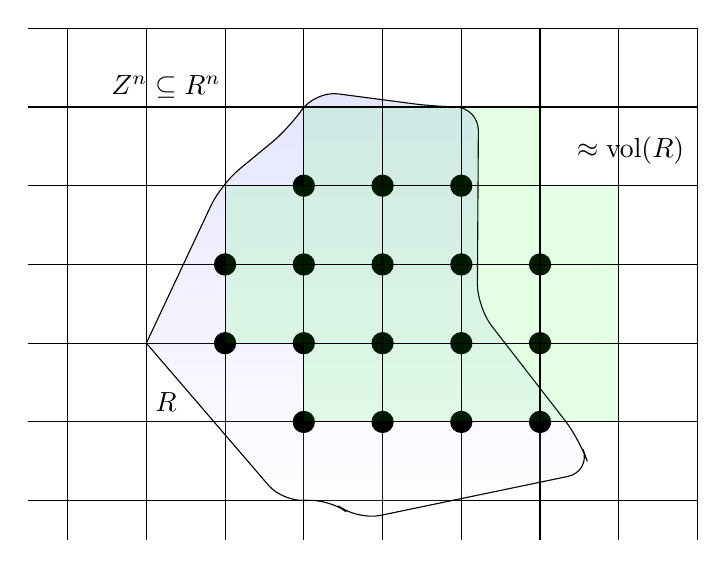
\begin{tikzpicture}
\draw[step=1.0,black,thin] (0.5,0.5) grid (9,7);

 \draw [shade,
        top color=blue,
        bottom color=white,
        fill opacity=.1,
        decoration={random steps,segment length=2cm,amplitude=.75cm},
        decorate,
        rounded corners=.3cm]
     (2, 3) -- (4,6)   -- (6,6) -- (7.6,1.5) -- (4, 1) -- (2, 3);

\node[fill=black, circle, inner sep=0.1cm] at (4,2) {};
\node[fill=black, circle, inner sep=0.1cm] at (5,2) {};
\node[fill=black, circle, inner sep=0.1cm] at (6,2) {};
\node[fill=black, circle, inner sep=0.1cm] at (7,2) {};

\node[fill=black, circle, inner sep=0.1cm] at (3,3) {};
\node[fill=black, circle, inner sep=0.1cm] at (4,3) {};
\node[fill=black, circle, inner sep=0.1cm] at (5,3) {};
\node[fill=black, circle, inner sep=0.1cm] at (6,3) {};
\node[fill=black, circle, inner sep=0.1cm] at (7,3) {};


\node[fill=black, circle, inner sep=0.1cm] at (3,4) {};
\node[fill=black, circle, inner sep=0.1cm] at (4,4) {};
\node[fill=black, circle, inner sep=0.1cm] at (5,4) {};
\node[fill=black, circle, inner sep=0.1cm] at (6,4) {};
\node[fill=black, circle, inner sep=0.1cm] at (7,4) {};


\node[fill=black, circle, inner sep=0.1cm] at (4,5) {};
\node[fill=black, circle, inner sep=0.1cm] at (5,5) {};
\node[fill=black, circle, inner sep=0.1cm] at (6,5) {};

\draw[draw=black, fill=green, fill opacity=0.1] (4, 2) rectangle ++(1,1);
\draw[draw=black, fill=green, fill opacity=0.1] (5, 2) rectangle ++(1,1);
\draw[draw=black, fill=green, fill opacity=0.1] (6, 2) rectangle ++(1,1);
\draw[draw=black, fill=green, fill opacity=0.1] (7, 2) rectangle ++(1,1);

\draw[draw=black, fill=green, fill opacity=0.1] (3, 3) rectangle ++(1,1);
\draw[draw=black, fill=green, fill opacity=0.1] (4, 3) rectangle ++(1,1);
\draw[draw=black, fill=green, fill opacity=0.1] (5, 3) rectangle ++(1,1);
\draw[draw=black, fill=green, fill opacity=0.1] (6, 3) rectangle ++(1,1);
\draw[draw=black, fill=green, fill opacity=0.1] (7, 3) rectangle ++(1,1);

\draw[draw=black, fill=green, fill opacity=0.1] (3, 4) rectangle ++(1,1);
\draw[draw=black, fill=green, fill opacity=0.1] (4, 4) rectangle ++(1,1);
\draw[draw=black, fill=green, fill opacity=0.1] (5, 4) rectangle ++(1,1);
\draw[draw=black, fill=green, fill opacity=0.1] (6, 4) rectangle ++(1,1);
\draw[draw=black, fill=green, fill opacity=0.1] (7, 4) rectangle ++(1,1);


\draw[draw=black, fill=green, fill opacity=0.1] (4, 5) rectangle ++(1,1);
\draw[draw=black, fill=green, fill opacity=0.1] (5, 5) rectangle ++(1,1);
\draw[draw=black, fill=green, fill opacity=0.1] (6, 5) rectangle ++(1,1);

\node at (2.25, 2.25) {$R$};

\node at (8.15, 5.45) {$\approx\mathrm{vol}(R)$};

\node at (2.25, 6.25) {${\mathbb{Z}}^n \subseteq {\mathbb{R}}^n$};

\end{tikzpicture}
}
\end{figure}

This isn't exactly right, but would become closer as \(R\) grew larger,
and the correction term comes from edge effects. For
\(R \subseteq {\mathbb{R}}^n\) and \(t\in {\mathbb{R}}\), define the
dilation
\begin{align*}
tR \coloneqq\left\{{ t\mathbf{x} {~\mathrel{\Big|}~}\mathbf{x} \in R }\right\} 
.\end{align*}

\end{remark}

\begin{theorem}[?]

Let \(R\) be a region in \({\mathbb{R}}^n\) which is \emph{Riemann
measurable}.\footnote{This means that \(\chi_R\) should be Riemann
  integrable, i.e.~the bounded region is contained in a rectangle, and
  integrals over such rectangles converges to what we'll call the
  volume.} Then the number of lattice points satisfies
\begin{align*}
{1\over t^n} \sum_{\mathbf{v} \in {\mathbb{Z}}^n} \chi_{tR} (\mathbf{v})
\overset{t\to \infty }\to \operatorname{vol}(R)
.\end{align*}

\end{theorem}

\begin{proof}[?]

Notice that the left-hand side can be written as
\begin{align*}
{1\over t^n} \sum_{\mathbf{v} \in {\mathbb{Z}}^n} \chi_{tR} (\mathbf{v})
=
{1\over t^n} = \sum_{\mathbf{w} \in t^{-1}{\mathbb{Z}}^n} \chi_R(\mathbf{w})
.\end{align*}
This has the effect of making the squares partitioning
\({\mathbb{R}}^n\) finer, the right-hand side is literally the Riemann
sum for
\begin{align*}
\int \chi_R(\mathbf{w}) \,d \mathbf{w} \coloneqq\operatorname{vol}(R)
.\end{align*}

\end{proof}

\begin{remark}

Note that there is a small technicality since \(t\) can take on
non-integer values, but the limiting behavior is the same. Next time:
we've seen that the number of lattice points is sometimes
well-approximated by volume, but it's possible to have regions of
unbounded volume with no lattice points, e.g.~by taking a large ball and
deleting all lattice points. It would be nice to have a theorem which
guarantee when a region will have lattice points, and Minkowski's
theorem will be one such theorem we'll look at next time.

\end{remark}

\hypertarget{ch.-12-lattice-points-monday-march-01}{%
\section{Ch. 12: Lattice Points (Monday, March
01)}\label{ch.-12-lattice-points-monday-march-01}}

\hypertarget{minkowski-version-1}{%
\subsection{Minkowski (Version 1)}\label{minkowski-version-1}}

\begin{remark}

Basic heuristic from last time: counting the lattice points in a region
\(R\) should be approximately \(\operatorname{vol}(R)\). We turned this
into a theorem for certain regions:

\end{remark}

\begin{theorem}[?]

Let \(R \subseteq {\mathbb{R}}^n\) be a bounded region with a
well-defined with respect to the Riemann integral. Letting \(L_{R}\) be
the number of lattice points in \(R\), we have
\begin{align*}
{1\over t^n} L_{tR} \overset{t\to \infty}\to \operatorname{vol}(R)
.\end{align*}

\end{theorem}

\begin{remark}

Most of today: Minkowski's theorem, which will guarantee a lattice point
under some conditions.

\end{remark}

\begin{theorem}[Minkowski (Version 1)]

Let \(R \subseteq {\mathbb{R}}^n\) be a bounded region that is

\begin{enumerate}
\def\labelenumi{\arabic{enumi}.}
\item
  Convex, so any line segment connecting two points in \(R\) is entirely
  contained within \(R\), and
\item
  Symmetric about \(\mathbf{0}\), so
  \(\mathbf{x}\in R\implies -\mathbf{x}\in R\).
\end{enumerate}

If \(\operatorname{vol}(R) > 2^n\), then \(R\) contains a nonzero
lattice point.

\end{theorem}

\begin{remark}

Any circle/ball or ellipse will be an example. Note that \(2^n\) is
sharp, i.e.~this theorem does not hold for a smaller constant: take the
square \((-1, 1) \times(-1, 1) \subseteq {\mathbb{R}}^2\), which has
volume 4 but only contains the origin as a lattice point.

\end{remark}

\begin{proof}[?]

Note that any such region already contains \(\mathbf{0}\), since
containing \(\mathbf{x}\) and \(-\mathbf{x}\) plus convexity implies
containing the line between them, which passes through \(\mathbf{0}\).
By assumption \(\operatorname{vol}(R) > 2^n\), and hence
\((1/t^n)L_{tR} > 2^n\) for \(t\) large enough. So set \(t=m\) for some
\(m>> 1\in {\mathbb{Z}}^{\geq 0}\), this yields \(L_{mR} > (2m)^n\).
Consider \({\mathbb{Z}}^n\) and taking all coordinates \(\pmod 2m\).
This yields \((2m)^n\) equivalence classes of points, so by the
pigeonhole principle there exist
\(\mathbf{v}_1 \neq \mathbf{v}_2 \in mR\) such that
\((\mathbf{v}_1 - \mathbf{v}_2)/2m \in {\mathbb{Z}}^n\), and the claim
is that this is the lattice point we want. Note that this is nonzero,
why is it in the region \(R\)? By definition,
\((1/m)\mathbf{v}_1 \in R\) and \((-1/m)\mathbf{v}_2 \in R\) using the
symmetric assumption. The midpoint between these is precisely the
previous point, and this is in \(R\) by convexity.

\end{proof}

\hypertarget{minkowski-version-2}{%
\subsection{Minkowski (Version 2)}\label{minkowski-version-2}}

\begin{definition}[Lattice]

A \textbf{lattice} in \({\mathbb{R}}^n\) is the
\({\mathbb{Z}}{\hbox{-}}\)span of a collection of
\({\mathbb{R}}{\hbox{-}}\)linearly independent vectors in
\({\mathbb{R}}^n\).

\end{definition}

\begin{example}[$n=2$]

\envlist

\begin{itemize}
\tightlist
\item
  \(\Lambda \coloneqq{\mathbb{Z}}{\left[ {1, 0} \right]}^t + {\mathbb{Z}}\left\{{0, 1}\right\}^t\).
  This tiles the plane by squares.
\item
  \(\Lambda \coloneqq{\mathbb{Z}}{\left[ {1, 1} \right]}^t + {\mathbb{Z}}\left\{{1, 3}\right\}^t\).
  Note that this now tiles the plane by parallelograms:
\end{itemize}

\begin{figure}
\centering
\resizebox{\columnwidth}{!}{%
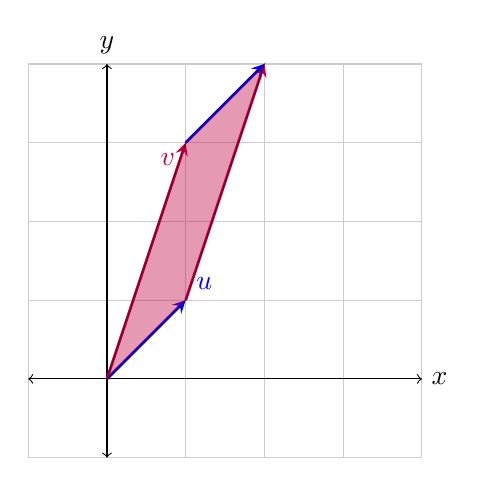
\begin{tikzpicture}
  \draw[thin,gray!40] (-1,-1) grid (4,4);
  \draw[<->] (-1,0)--(4,0) node[right]{$x$};
  \draw[<->] (0,-1)--(0,4) node[above]{$y$};
  \draw[line width=1pt,blue,-stealth](0,0)--(1,1) node[anchor=south west]{$\boldsymbol{u}$};
  \draw[line width=1pt,purple,-stealth](1,1)--(2,4) node[anchor=south west]{};
  \draw[line width=1pt,purple,-stealth](0,0)--(1,3) node[anchor=north east]{$\boldsymbol{v}$};
\draw[line width=1pt,blue,-stealth](1,3)--(2,4) node[anchor=south west]{};

\draw [draw=black, fill=purple, opacity=0.4]
       (0,0) -- (1,1) -- (2,4) -- (1,3) -- cycle;
\end{tikzpicture}
}
\end{figure}

\begin{itemize}
\tightlist
\item
  \(\Lambda \coloneqq{\mathbb{Z}}{\left[ {1, 0} \right]}^t\), which
  recovers \({\mathbb{Z}}\subseteq {\mathbb{R}}\). This is not a full
  lattice, since it lies in a proper subspace of \({\mathbb{R}}^2\).
\end{itemize}

Note that this will always result in a free abelian group on \(n\)
generators. Why not define a lattice this way? Here's a non-example:

\begin{itemize}
\tightlist
\item
  \(\Lambda \coloneqq{\mathbb{Z}}{\left[ {\sqrt{2} , 0} \right]}^t + {\mathbb{Z}}\left\{{1, 0}\right\}^t\),
  which are not linearly independent over \({\mathbb{R}}\). This yields
  a dense set of points on the real axis in \({\mathbb{R}}^2\), and is
  still a free abelian group of rank 2. We'll see later that no lattice
  can be dense, and in fact they must always be discrete.
\end{itemize}

\end{example}

\begin{remark}

It may not be obvious that a lattice has a uniquely determined number of
generating elements. This turns out to be true: if
\(\Lambda = \sum_{i=1}^d {\mathbb{Z}}\mathbf{v}_i\) with
\(\left\{{ \mathbf{v}_i }\right\}_{i=1}^d\) linearly independent over
\({\mathbb{R}}\), then
\(\Lambda\otimes_{\mathbb{Z}}{\mathbb{R}}\cong \sum_{i=1}^d {\mathbb{R}}\mathbf{v}_i \cong {\mathbb{R}}^d\),
which is now an \({\mathbb{R}}{\hbox{-}}\)vector vector space of real
dimension \(d\). Noting that
\(\dim_{\mathbb{R}}(\Lambda\otimes_{\mathbb{Z}}{\mathbb{R}})\) doesn't
depend on the choice of basis, any different choice of generating set
for \(\Lambda\) must have the same number of generators.

\end{remark}

\begin{definition}[Full Lattices]

If \(d=n\), we'll call \(\Lambda\) a \textbf{full lattice}.

\end{definition}

\begin{definition}[Fundamental Parallelepiped]

Note that if \(\Lambda\) is full, then
\(\Lambda= \sum_{i=1}^n {\mathbb{Z}}\mathbf{v}_i\) with the
\(\mathbf{v}_i\) linearly independent over \({\mathbb{R}}\). We define
the \textbf{fundamental parallelepiped} as the set
\begin{align*}
\left\{{ \sum_{i=1}^n c_n \mathbf{v}_n {~\mathrel{\Big|}~}0 \leq c_i \leq 1}\right\} 
.\end{align*}
Note that this depends on the choice of generating set.

\end{definition}

\begin{example}[?]

For \(\mathbf{v}_1 = {\left[ {1, 1} \right]}^t\) and
\(\mathbf{v}_2 = {\left[ {1, 3} \right]}\), we get the parallelogram
shown in the earlier figure. Note that \(\Lambda\) is also generated by
\(\mathbf{v}_1 = \left\{{1, 1}\right\}, \mathbf{w}_2 = {\left[ {0, 2} \right]}\),
but this generates a different parallelepiped:

\begin{figure}
\centering
\resizebox{\columnwidth}{!}{%
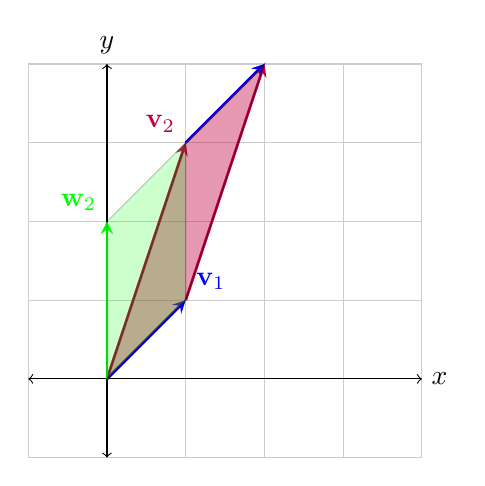
\begin{tikzpicture}
  \draw[thin,gray!40] (-1,-1) grid (4,4);
  \draw[<->] (-1,0)--(4,0) node[right]{$x$};
  \draw[<->] (0,-1)--(0,4) node[above]{$y$};
  \draw[line width=1pt,blue,-stealth](0,0)--(1,1) node[anchor=south west]{$\mathbf{v}_1$};
  \draw[line width=1pt,purple,-stealth](1,1)--(2,4) node[anchor=south west]{};
  \draw[line width=1pt,purple,-stealth](0,0)--(1,3) node[anchor=south east]{$\mathbf{v}_2$};
\draw[line width=1pt,blue,-stealth](1,3)--(2,4) node[anchor=south west]{};

\draw[line width=1pt,green,-stealth](0,0)--(0,2) node[anchor=south east]{$\mathbf{w}_2$};

\draw [draw=black, fill=purple, opacity=0.4]
       (0,0) -- (1,1) -- (2,4) -- (1,3) -- cycle;

\draw [draw=black, fill=green, opacity=0.2]
       (0,0) -- (1,1) -- (1,3) -- (0,2) -- cycle;
\end{tikzpicture}
}
\end{figure}

\end{example}

\begin{proposition}[?]

In general, one gets a parallelotope whose volume is an invariant of the
lattice itself.

\end{proposition}

\begin{proof}[of proposition]

How do we compute this? Let
\(M_v = {\left[ { \mathbf{v}_1^t, \cdots, \mathbf{v}_n^t} \right]}\) be
the linear transformation obtained by placing all of the generating
vectors into the columns of a matrix, and consider scaling the unit cube
\(C = [0, 1]^n\). Then letting \(P\) be the fundamental parallelepiped,
we have \(P = M_v C\) and so
\begin{align*}
\operatorname{vol}(P) = \operatorname{vol}(M_v C) = {\left\lvert { \det(M_v) } \right\rvert} \operatorname{vol}(C) = \det(M_v)
,\end{align*}
using that the volume of the standard cube is 1. So it suffices to check
that if \(\mathbf{v}_i\) and \(\mathbf{w}_j\) generate the same lattice
\(\Lambda\), then \(\det M_v = \det M_w\). Why is this true? If they
generate the same lattice, every \(\mathbf{v}_i\) is a
\({\mathbb{Z}}{\hbox{-}}\)linear combination of the \(\mathbf{w}_j\),
and similarly every \(\mathbf{w}_j\) can be written as a linear
combination of the \(\mathbf{v}_i\). So we get
\begin{align*}
M_v = M_w A
\qquad 
M_w = M_v A'
\end{align*}
for some matrices \(A, A'\). We can thus write
\begin{align*}
M_v = M_vA' A
.\end{align*}
. Since the \(\mathbf{v}_i\) are linearly independent, \(M_v\) is
invertible, so right-multiplying yields \(AA' = I\) and taking
determinants yields
\begin{align*}
1 = \det(A')\det(A)
.\end{align*}
Noting that \(A, A' \in \operatorname{Mat}(n\times n, {\mathbb{Z}})\),
their determinants must be integers, which forces
\(\det(A) = \det(A') = \pm 1\). Taking determinants in the original
equation yields
\begin{align*}
\det(M_v) = \det(A) \det(M_w) = \pm \det(M_w)
,\end{align*}
and taking absolute values yields the result.

\end{proof}

\begin{definition}[Covolume of a Lattice]

We'll call the common value \({\left\lvert {\det M_v} \right\rvert}\)
for any choice of generating set \(\left\{{ \mathbf{v}_i }\right\}\) the
\textbf{covolume} of \(\Lambda\):
\begin{align*}
\operatorname{covol}( \Lambda) \coloneqq{\left\lvert { \det M_v } \right\rvert}
.\end{align*}

\end{definition}

\begin{theorem}[Minkowski (Version 2)]

Let \(\Lambda\) be a full lattice in \({\mathbb{R}}^n\), and let
\(R \subseteq {\mathbb{R}}^n\) be a region that is convex and symmetric
about zero. Assume that
\begin{align*}
\operatorname{vol}(R) > 2^n \operatorname{covol}( \Lambda)
.\end{align*}
Then \(R\) contains a nonzero \(\mathbf{v} \in \Lambda\).

\end{theorem}

\begin{remark}

Taking \(\Lambda\coloneqq{\mathbb{Z}}^n\) recovers the first version.
Idea of proof: any full lattice is the image of the standard lattice
under some linear transformation.

\end{remark}

\begin{proof}[?]

Let \(\mathbf{v}_1, \cdots, \mathbf{v}_n\) be \(n\) generators for
\(\Lambda\), then define a linear transformation
\begin{align*}
T: {\mathbb{R}}^n &\to {\mathbb{R}}^n \\
\mathbf{v}_i &\mapsto \mathbf{e}_i
,\end{align*}
which takes each generator to the corresponding standard basis vector.
The \(T \Lambda = {\mathbb{Z}}^n\) is the standard lattice, and
\begin{align*}
\operatorname{vol}(T(R)) = {\left\lvert { \det(T) } \right\rvert} \operatorname{vol}(R) = {\operatorname{vol}(R) \over \operatorname{covol}( \Lambda) } > 2^n
,\end{align*}
noting that
\(T^{-1}= {\left[ {\mathbf{v}_1^t, \cdots, \mathbf{v}_n^t} \right]}\).
Now applying the original Minkowski theorem we get a nonzero point
\begin{align*}
\mathbf{x}\in {\mathbb{Z}}^n \cap T(R)
\implies T^{-1}\mathbf{x} \in \Lambda \cap R
.\end{align*}

\end{proof}

\hypertarget{application-the-4-square-theorem}{%
\subsubsection{Application: The 4 Square
Theorem}\label{application-the-4-square-theorem}}

\begin{theorem}[4 Square Theorem (Lagrange)]

Every positive integer is a sum of 4 squares of integers.

\end{theorem}

\begin{lemma}[?]

Let \(m \in {\mathbb{Z}}^{>0}\) be squarefree, then there are
\(A, B \in {\mathbb{Z}}\) such that
\begin{align*}
A^2 + B^2 + 1 \equiv 0 \pmod m
,\end{align*}
i.e.~\(-1\) is always the sum of two squares in the ring
\({\mathbb{Z}}/m\).

\end{lemma}

\begin{proof}[?]

We're trying to solve an equation \(\pmod m\), and by the CRT it
suffices to solve it for every prime power dividing \(m\), and since
\(m\) is squarefree, all prime powers occur with exponent 1. So it
suffices to consider \(m=p\) a prime. We can further assume \(p\) is
odd, since if \(p=2\) we can take \(A=1, B=2\). Consider the following
two subsets of \({\mathbb{Z}}/p\):
\begin{align*}
S_1 &\coloneqq\left\{{ A^2 \pmod p }\right\} \\
S_2 &\coloneqq\left\{{ -1-B^2 \pmod p }\right\} 
.\end{align*}
Note that \(\# S_1 = {p+1 \over 2}\), since the number of nonzero
squares is half the number of elements, so \({p-1\over 2}\), and we add
in zero. Similarly \(\# S_2 = \# S_1\) since it can be obtained from
\(S_1\) by sending \(x\mapsto -1-x\). Note that
\({p+1\over 2} > {p\over 2}\), but
\({\left\lvert {{\mathbb{Z}}/p} \right\rvert} = p\), so these two sets
can't be disjoint. So there is some \(A^1 = -1-B^2 \pmod p\).

\end{proof}

\begin{proof}[of the 4 Square Theorem]

Suppose \(m\) is squarefree. Choose \(A, B\) as in the lemma, so
\(A^2 + B^2 \equiv -1 \pmod m\), and define
\(\gamma \coloneqq A+ Bi \in {\mathbb{Z}}[i]\). Let
\begin{align*} \Lambda \coloneqq\left\{{ (\alpha, \beta) \in {\mathbb{Z}}[i] {~\mathrel{\Big|}~}\alpha\equiv \beta \gamma \pmod m }\right\} .\end{align*}
Taking one such ordered pair in \(\Lambda\), we can apply complex
conjugation to obtain
\begin{align*}
\alpha\equiv \beta \gamma\pmod m \implies {\overline{{ \alpha}}} {\overline{{ \beta}}} {\overline{{ \gamma}}} \pmod{\overline{{m}}} = m
,\end{align*}
where we can immediately note that \({\overline{{m}}} = m\) since
\(m\in {\mathbb{Z}}\). Multiplying these two congruences yields
\begin{align*}
\alpha{\overline{{\alpha}}} 
= N( \alpha) 
\equiv N( \beta) N( \gamma) \pmod m
\equiv - N( \beta) \pmod m
,\end{align*}
and so we have \(N( \alpha) + N( \beta) \equiv 0 \pmod m\). But these
are Gaussian integers, so writing \(\alpha = a + bi, \beta = c + di\) we
obtain
\begin{align*}
a^2 + b^2 + c^2 + d^2 = \equiv 0 \pmod m
.\end{align*}
Being congruent to \(0\pmod m\) in \({\mathbb{Z}}[i]\) means that both
the real and imaginary parts are divisible by \(m\), but since the
left-hand side above is an ordinary integer, it has no imaginary part.
So \(m \mathrel{\Big|}a^2 + b^2 + c^2 + d^2\) for every element of
\(\Lambda\). Noting that \(\Lambda \subseteq {\mathbb{Z}}[i]\) we can
identify \(\Lambda \subseteq {\mathbb{Z}}^4 \subseteq {\mathbb{R}}^4\)
by pairing \(( \alpha, \beta) \rightleftharpoons(a,b,c,d)\).

\begin{claim}

\(\Lambda\subseteq {\mathbb{R}}^4\) is a full lattice, and after writing
a set of generators and computing the determinant, one finds that
\(\operatorname{covol}( \Lambda) = m^2\).

\end{claim}

\begin{quote}
See the book for a proof of this claim!
\end{quote}

Now let
\begin{align*}
R \coloneqq\left\{{ {\left[ {x,y,z,w} \right]} \in {\mathbb{R}}^4 {~\mathrel{\Big|}~}x^2 + y^2 + z^2 + w ^2 < 2m  }\right\}
,\end{align*}
which is a convex and centrally symmetric region. A multivariable
Calculus exercise shows \(\operatorname{vol}(R) = 2\pi^2 m^2\), and
\(2\pi^2 > 2^4 \operatorname{covol}( \Lambda)\). Applying Minkowski
version 2, there exists a nonzero point
\(\mathbf{x} \in R \cap\Lambda\), and thus its coordinates satisfy
\begin{align*}
0 < x^2 + y^2 + z^2 + w^2 < 2m
.\end{align*}
The middle term is then an integer that is a multiple of \(m\), forcing
it to be equal to \(m\).

\end{proof}

\begin{remark}

We made the assumption that \(m\) was squarefree, but we can write any
\(m\in {\mathbb{Z}}^{>0}\) as \(m = k^2 m'\) where \(m'\) is squarefree.
Then writing \(m' = x^2 + y^2 + z^2 + w^2\), we have
\begin{align*} m = (kx)^2 + (ky)^2 + (kz)^2 + (kw)^2 \end{align*}
. There are other applications of Minkowski's theorem that tell you when
certain types of numbers are represented by special quadratic forms
(such as the above sum of squares). See Pete Clark's papers!

\end{remark}

\addsec{ToDos}
\listoftodos[List of Todos]
\cleardoublepage

% Hook into amsthm environments to list them.
\addsec{Definitions}
\renewcommand{\listtheoremname}{}
\listoftheorems[ignoreall,show={definition}, numwidth=3.5em]
\cleardoublepage

\addsec{Theorems}
\renewcommand{\listtheoremname}{}
\listoftheorems[ignoreall,show={theorem,proposition}, numwidth=3.5em]
\cleardoublepage

\addsec{Exercises}
\renewcommand{\listtheoremname}{}
\listoftheorems[ignoreall,show={exercise}, numwidth=3.5em]
\cleardoublepage

\addsec{Figures}
\listoffigures
\cleardoublepage


\printbibliography[title=Bibliography]


\end{document}
